\chapter{
Beyond SBDRL II: local algebras
(V1.1)
}

%%%%%%%%%%%%%%%%%%%%%%%%%%%%%%%%%
\section{
A local equivalence
}
\draftnote{green}{Include}{
\begin{enumerate}
    \item General properties of $(\hat{A}^{*}, \circ_{\sim_{w}})$.
\end{enumerate}
}

\begin{definition}[Local equivalence of actions under $\sim_{w}$]
	Given two actions $a, a' \in \hat{A}^{*}$ and a world state $w \in W$,
	\begin{equation}
		a \sim_{w} a' \iff a \ast w = a' \ast w
	\end{equation}
\end{definition}

\begin{propositionE}
    $\sim_{w}$ is an equivalence relation.
\end{propositionE}
\begin{proofE}
    To prove that $\sim_{w}$ is an equivalence relation on the set $\hat{A}^{*}$, we need to show that $\sim_{w}$ is (1) reflexive, (2) symmetric, and (3) transitive.
    \begin{enumerate}
        \item \textbf{Reflexive.}
        We need to show that $a \sim_{w} a$ for all $a \in \hat{A}^{*}$.
        By the definition of $\sim_{w}$, we need to check if $a \ast w = a \ast w$, which is true by equality.

        \item \textbf{Symmetric.}
        We need to show that if $a \sim_{w} a'$, then $a' \sim_{w} a$.
        If $a \sim_{w} a'$ then, by the definition of $\sim_{w}$, we have $a \sim_{w} a' \iff a \ast w = a' \ast w$.
        Therefore, we have that $a' \ast w = a \ast w$, and so, from the definition of $\sim_{w}$, we have $a' \sim_{w} a$.

        \item \textbf{Transitive.}
        We need to show that if $a \sim_{w} a'$ and $a' \sim_{w} a''$, then $a \sim_{w} a''$.
        Let $a \sim_{w} a'$ and $a' \sim_{w} a''$.
        By definition of $\sim_{w}$ we have $a \ast w = a' \ast w$ and $a' \ast w = a'' \ast w$.
        By transitivity of equality, we have $a \ast w = a'' \ast w$, which means $a \sim_{w} a''$.
    \end{enumerate}
\end{proofE}

\begin{propositionE}\label{prp:global_equivalence_implies_local_equivalence}
    For all $a, a' \in \hat{A}^{*}$,
    \begin{equation}
        a \sim a' \implies a \sim_{w} a' \quad \text{for all $w \in W$}
    \end{equation}
\end{propositionE}
\begin{proofE}
    If $a \sim a'$, then
    \begin{equation}
        \label{eqn:local_global_equivalence_1}
        a \ast w = a' \ast w \quad \text{for all $w \in W$}
    \end{equation}
    Select an arbitrary $w_{0} \in W$.
    From \cref{eqn:local_global_equivalence_1}, we have
    \begin{equation}
        a \ast w_{0} = a' \ast w_{0}
    \end{equation}
    By definition of local equivalence, we have
    \begin{equation}
        a \sim_{w_{0}} a'
    \end{equation}
    Since $w_{0}$ was an arbitrary choice, this argument holds for all $w \in W$, and so we have
    \begin{equation}
        a \sim_{w} a' \quad \text{for all $w \in W$}
    \end{equation}
\end{proofE}


\begin{propositionE}\label{prp:gloabal_equivalence_is_local_equivalence_on_all_world_states}
    \begin{equation}
        a \sim a' \iff a \sim_{w} a' \quad \text{for all $w \in W$}
    \end{equation}
    \footnote{
    This means that $\sim$ is the intersection of all local equivalence relations
    \begin{equation}
        \sim \; = \bigcap_{w \in W} \sim_{w}
    \end{equation}
    \draftnote{blue}{Consider}{Can we draw this for our example ?}
    }
\end{propositionE}
\begin{proofE}
\begin{enumerate}
    \item \textbf{$a \sim a' \implies a \sim_{w} a'$ for all $w \in W$.}
    See \cref{prp:global_equivalence_implies_local_equivalence}.

    \item \textbf{$a \sim a' \impliedby a \sim_{w} a'$ for all $w \in W$.}
    If $a \sim_{w} a'$ for all $w \in W$, then
    \begin{equation}
        \label{eqn:local_global_equivalence_2}
        a \ast w = a' \ast w \quad \text{for all $w \in W$}
    \end{equation}
    \cref{eqn:local_global_equivalence_2} is the definition of $a \sim a'$.
\end{enumerate}
\end{proofE}

\draftnote{blue}{Move this?}{}
For a world state $w$ of a world $\mathscr{W}$, let $(\hat{A}^{*}/\sim)_{w}$ denote the set $\hat{A}^{*}/\sim$ of equivalence classes of $\hat{A}^{*}$ under the global equivalence $\sim$ for the reachable subworld $\mathscr{W}^{\hat{A}\to}(w)$ from $w$.


\begin{propositionE}\label{prp:local_class_is_disjoint_union_of_global_classes}
    Every local equivalence class $[a]_{\sim_{w}} \in \hat{A}^{*}/\sim_{w}$ is a disjoint union of global equivalence classes\footnote{
    In other words, each local equivalence class in $\hat{A}^{*}/\sim_{w}$ is made up of one or more global equivalence classes in $\hat{A}^{*}/\sim$ and each global equivalence class in is exactly one local equivalence class.
    }
    \begin{equation}
        [a]_{\sim_{w}} = \bigsqcup_{i \in I}[a_{i}]_{\sim}
    \end{equation}
    where $\{ [a_{i}]_{\sim} \}_{i \in I} \subseteq \hat{A}^{*}/\sim$ and $[a_{i}]_{\sim} \subseteq [a]_{\sim_{w}}$ for all $i \in I$.
    \footnote{
    $I$ is the index set that labels all global equivalence classes contained in $[a]_{\sim_{w}}$:
    \begin{equation}
        I := \{ i \mid [a_{i}]_{\sim} \subseteq [a]_{\sim_{w}} \}
    \end{equation}
    }
\end{propositionE}
\begin{proofE}
\begin{enumerate}
    \item \textbf{Global equivalence $\implies$ local equivalence.}
    From \cref{prp:global_equivalence_implies_local_equivalence} we have
    \begin{align}
        & a \sim a' \implies a \sim_{w} a' \\
        \implies & [a]_{\sim} \subseteq [a]_{\sim_{w}}
    \end{align}
    Therefore, each global equivalence class $[a_{i}]_{\sim}$ is contained entirely within a single local equivalence class $[a]_{\sim_{w}}$.
    Since each $[a_{i}]_{\sim} \subseteq [a]_{\sim_{w}}$, the union of all the $[a_{i}]_{\sim}$ contained in a specific $[a]_{\sim_{w}}$ is also contained in $[a]_{\sim_{w}}$.
    Therefore, we have
    \begin{equation}\label{eqn:subset1}
        \bigcup_{i \in I}[a_{i}]_{\sim} \subseteq [a]_{\sim_{w}}
    \end{equation}

    \item \textbf{Equality of sets.}
    For any $a' \in [a]_{\sim_{w}}$, we have $a' \sim_{w} a$ by definition.
    Since $a' \sim_{w} a$, we have $[a']_{\sim} \subseteq [a]_{\sim_{w}}$ (from step 1 of this proof).
    The index set $I$ labels all the global equivalence classes contained in $[a]_{\sim_{w}}$:
    \begin{equation}
        I = \{ i \mid [a_{i}]_{\sim} \subseteq [a]_{\sim_{w}} \}
    \end{equation}
    $I$ is well-defined because each global class is contained in exactly one local class.
    Since $[a']_{\sim} \subseteq [a]_{\sim_{w}}$, $[a']_{\sim}$ is one of the classes $[a_{i}]_{\sim}$ indexed by $I$.
    Therefore, $[a']_{\sim} \subseteq \bigcup_{i \in I}[a_{i}]_{\sim}$.
    Since $a' \in [a']_{\sim}$, we have $a' \in \bigcup_{i \in I}[a_{i}]_{\sim}$.
    Since $a'$ was an arbitrary element in $[a]_{\sim_{w}}$, we have
    \begin{equation}\label{eqn:subset2}
        [a]_{\sim_{w}} \subseteq \bigcup_{i \in I}[a_{i}]_{\sim}
    \end{equation}
    Combining \cref{eqn:subset1,eqn:subset2} gives
    \begin{equation}
        [a]_{\sim_{w}} = \bigcup_{i \in I}[a_{i}]_{\sim}
    \end{equation}
    
    \item \textbf{Disjointness of global equivalence classes.}
    \begin{enumerate}
        \item \textbf{Claim.}
        If $[a_{i}]_{\sim}$ and $[a_{j}]_{\sim}$ are distinct global equivalence classes contained within the same local equivalence class $[a]_{\sim_{w}}$, then they are disjoint
        \begin{equation}
            [a_{i}]_{\sim} \cap [a_{j}]_{\sim} = \emptyset
        \end{equation}

        \item \textbf{Proof by contradiction.}
        Assume that $[a_{i}]_{\sim}$ and $[a_{j}]_{\sim}$ are distinct global equivalence classes with a common element $b \in \hat{A}^{*}$ such that $b \in [a_{i}]_{\sim} \cap [a_{j}]_{\sim}$.
        By definition of equivalence classes, we have
        \begin{align}
            & b \in [a_{i}]_{\sim} \implies b \sim a_{i} \\
            & b \in [a_{j}]_{\sim} \implies b \sim a_{j}
        \end{align}
        By transitivity of $\sim$, we have
        \begin{align}
            & a_{i} \sim b \sim a_{j} \\
            \implies & a_{i} \sim a_{j} \\
            \implies & [a_{i}]_{\sim} = [a_{j}]_{\sim}
        \end{align}
        This contradicts that $[a_{i}]_{\sim}$ and $[a_{j}]_{\sim}$ are distinct.
    \end{enumerate}

    \item \textbf{Conclusion.}
    The union $\bigcup_{i \in I}[a_{i}]_{\sim}$ is (1) equal to $[a]_{\sim_{w}}$, and (2) disjoint.
    Therefore, we have
    \begin{equation}
        [a]_{\sim_{w}} = \bigsqcup_{i \in I}[a_{i}]_{\sim}
    \end{equation}
\end{enumerate}
\end{proofE}

\begin{corollary}
    For a world state $w \in W$ in a world $\mathscr{W}$,
    \begin{equation}
        |(\hat{A}^{*}/\sim)_{w}| \geq | \hat{A}^{*}/\sim_{w}|
    \end{equation}
\end{corollary}


\draftnote{blue}{Footnote}{
The global equivalence $\sim$ is a refinement of the local equivalences $\sim_{w}$ for $w \in W$; this means that globally equivalent actions must be locally equivalence, but locally equivalent action do not need to be globally equivalent.
\begin{align}
    a \sim a' & \implies a \sim_{w} a' \\
    a \sim_{w} a' & \centernot\implies a \sim a'
\end{align}
}



We attempt to define our induced composition operator $\circ_{\sim_{w}}$ on the quotient set $\hat{A}^{*}/\sim_{w}$ in a similar way to how we defined the composition operator $\circ_{\sim}$ for our global equivalence relation $\sim$:
\begin{equation}
\begin{aligned}
    \circ_{\sim_{w}}: \; &(\hat{A}^{*}/\sim_{w}) \times (\hat{A}^{*}/\sim_{w}) \to (\hat{A}^{*}/\sim_{w}) \quad \text{such that}\\
    & [a']_{\sim_{w}} \circ_{\sim_{w}} [a]_{\sim_{w}} := [a' \circ a]_{\sim_{w}}
\end{aligned}
\end{equation}


%%%%%%%%%%%%%%%%%%%%%%%%%%%%%%%%%%%%%%%%%%%%%
\section{Local algebra algorithm}
\draftnote{green}{Include}{
\begin{enumerate}
        \item (?) Put the full algorithm in the appendices.
        \item CODE: well-definedness checker ?
\end{enumerate}
}

As with $\sim$, we developed an algorithm to construct the quotient set $\hat{A}^{*}/\sim_{w}$ and construct a Cayley table of the algebra $(\hat{A}^{*}/\sim_{w}, \circ_{\sim_{w}})$.

The latest version of the code for this section can be found at
\begin{center}
\url{https://github.com/awjdean/CayleyTableGeneration}
\end{center}

%%%%%%%%%%%%%%%%%%%%%%%%%%%%%%%%%%%%%%%%%%%%%
\subsection{Generating the equivalence classes}

To generate the local algebra, we altered algorithm \ref{alg:GenerateEquivClasses} to use a different $\Call{ComputeActionFunction}$ function.
Since our $\Call{LocalComputeActionFunction}$ requires an additional initial state parameter $w^{*}$, we must also feed that parameter into $\Call{GenerateEquivClasses}$ and $\Call{ProcessCandidate}$.
Other than those changes, the algorithm for generating the equivalence classes for the local algebra is the same as for the global algebra.

\begin{algorithm}[H]
	\caption{
		Compute the part of the action function $f_{a}: W \to W$ that sends $w^{*} \mapsto a \ast w^{*}$.
	}
    \label{alg:LocalComputeActionFunction}
	\hrulefill
	\begin{algorithmic}[1]
		\Procedure{LocalComputeActionFunction}{$a$, \; $\mathscr{W}$, \; $w^{*}$}
		\State $f_{a} \gets (\emptyset \to \emptyset)$
		\State $w_{a} \gets$ \Call{GenerateActionOutcome}{$a$, \; $w^{*}$, \; $\hat{\ast}$}
		\State $f_{a} \gets f_{a} \cup f_{a}'$ where $f_{a}': \{w^{*}\} \to \{w_{a}\}$ such that $f_{a}'(w^{*}) = w_{a}$
		\State \Return $f_{a}$
		\EndProcedure
	\end{algorithmic}
\end{algorithm}

%%%%%%%%%%%%%%%%%%%%%%%%%%%%%%%%%%%%%%%%%%%%%
\subsection{Generating the Cayley table}

To generate the local Cayley table, we use algorithm \ref{alg:GenerateCayley} with a different $\Call{ComputeCompositionActionFunction}$ function.

\begin{algorithm}[H]
	\caption{
		Compute the action function for the combination $l_{L} \circ l_{R}$ using \Call{LocalComputeActionFunction}.
	}
        \label{alg:ComputeCompositionActionFunction_local}
	\hrulefill
	\begin{algorithmic}[1]
		\Procedure{ComputeCompositionActionFunction}{$l_{L}$, \; $l_{R}$, \; $\mathcal{T}$, \; $\rho$, \; $\mathscr{W}$, \; $w^{*}$}
		      \State $a \gets \operatorname{Combine}(l_{L}, \; l_{R})$
                \State $f_{a} \gets$ \Call{LocalComputeActionFunction}{$a$, \; $\mathscr{W}$, \; $w^{*}$}
                \State \Return $f_{a}$
		\EndProcedure
	\end{algorithmic}
\end{algorithm}


%%%%%%%%%%%%%%%%%%%%%%%%%%%%%%%%%%%%%%%
\subsection{Mathematical analysis}

\begin{propositionE}\label{prp:local_algebra_cardinality}
The number of elements in $\hat{A}^{*}/\sim_{w}$ is the number of world states that are reachable from $w$.
    \begin{equation}
        |\hat{A}^{*}/\sim_{w}| = |W^{\hat{A}\to}(w)| \leq |W^{\bot}|
    \end{equation}
\end{propositionE}
\begin{proofE}
\begin{enumerate}
    \item \textbf{Define mapping between $\hat{A}^{*}/\sim_{w}$ and $W^{\hat{A}\to}(w)$.}
    We define the canonical mapping
    \begin{equation}
    \begin{aligned}
        & \phi: \hat{A}^{*}/\sim_{w} \to W^{\hat{A}\to}(w) \\
        & \phi([a]_{\sim_{w}}) = a \ast w
    \end{aligned}
    \end{equation}

    \item \textbf{Injectivity of $\phi$.}
    \begin{align}
        & \phi([a]_{\sim_{w}}) = \phi([a']_{\sim_{w}}) \\
        \implies & a \ast w = a' \ast w \\
        \implies & a \sim_{w} a' \\
        \implies & [a]_{\sim_{w}} = [a']_{\sim_{w}}
    \end{align}
    Therefore $\phi$ is injective.

    \item \textbf{Subjectivity of $\phi$.}
    Consider an arbitrary world state $w' \in W^{\hat{A}\to}(w)$.
    By the definition of $W^{\hat{A}\to}(w)$, there exists at least one action sequence $a \in \hat{A}^{*}$ such that $a \ast w = w'$.
    Therefore, $\phi([a]_{\sim_{w}}) = a \ast w = w'$.
    Since the choice of $w' \in W^{\hat{A}\to}(w)$ is arbitrary, there exists an equivalence class $[a]_{\sim_{w}} \in \hat{A}^{*}/\sim_{w}$ such that $\phi([a]_{\sim_{w}}) = w'$ for all world states in $W^{\hat{A}\to}(w)$.
    Therefore, $\phi$ is surjective.

    \item \textbf{Bijectivity of $\phi$}
    Since $\phi$ is injective and surjective, $\phi$ is bijective and therefore
    \begin{equation}
        |\hat{A}^{*}/\sim_{w}| = |W^{\hat{A}\to}(w)|
    \end{equation}
    $|W^{\hat{A}\to}(w)| \leq |W| + 1$ from the definition of $W^{\hat{A}\to}(w)$.
\end{enumerate}
\end{proofE}

\begin{propositionE}
    \Cref{alg:GenerateEquivClasses} with adjustments for the local equivalence $\sim_{w}$ (\cref{alg:LocalComputeActionFunction,alg:ComputeCompositionActionFunction_local}) always halts for finite $W$.
\end{propositionE}
\begin{proofE}
\begin{enumerate}
    \item \textbf{$|L|$ increases monotonically until its final iteration.}
    During each expansion iteration, the set $L$ either grows or remains the same.
    So at each expansion iteration, with a new distinct action is discovered and added to $L$ or no new distinct actions are discovered and the algorithm halts.

    \item \textbf{Upper bound on $|L|$.}
    Each equivalence class $[a]_{\sim_{w}} \in L$ is uniquely determined by its effect on $w^{*}$.
    For a world with $|W|$ world states there are at most $|W| + 1$ distinct transformations with a source of $w^{*}$ (one to every world state in $W^{\bot}$)\footnote{
    As we know from \cref{prp:local_algebra_cardinality} there are actually at most $|W^{\hat{A}\to}(w^{*})|$ distinct transformations with a source of $w^{*}$.
    }.
    Therefore, the set $L$ can have at most $|W|+1$ elements.

    \item \textbf{Halting.}
    If $L$ stops growing for one expansion iteration, then the algorithm halts.
    If $|L| = |W|+1$, then there are no more unique action functions and therefore no more distinct actions under $\sim_{w}$ and so \cref{alg:GenerateEquivClasses} halts.
    Since $|L|$ increases monotonically when it changes, either $|L|$ reaches $|W|+1$ and halts or the algorithm halts before $|L|=|W|+1$.
\end{enumerate}
\end{proofE}

\begin{propositionE}
    Consider \cref{alg:GenerateEquivClasses} with adjustments for the local equivalence $\sim_{w}$ (\cref{alg:LocalComputeActionFunction,alg:ComputeCompositionActionFunction_local}).
    When this algorithm halts, $L \cong \hat{A}^{*}/\sim_{w}$
\end{propositionE}
\begin{proofE}
    \textbf{Proof by contradiction.}
\begin{enumerate}
    \item \textbf{Set up.}
    Assume the algorithm halts with a set $L$, but there exists an undiscovered equivalence class $[b]_{\sim_{w}} \in \hat{A}^{*}/\sim_{w}$.
    Let $b$ be the shortest action such that $b \ast w^{*}$ is not represented in $L$ (i.e., $b$ is the shortest distinct action under $\sim_{w}$).

    \item \textbf{Decomposition of $b$.}
    We can write $b$ as $b = \hat{a} \circ b'$ where $\hat{a} \in \hat{A}/\sim_{w}$ and $b' \in \hat{A}^{\ast}$.
    Since $b$ is the shortest undiscovered distinct action under $\sim_{w}$, either $b'$ must have been discovered and be represented in $L$ or $b'$ is not discovered and $b$ is not the shortest undiscovered distinct action under $\sim_{w}$, since $b'$ is shorter than $b$, which is a contradiction.

    \item \textbf{Contradiction.}
    Given that $b'$ is known and represented in $L$, the algorithm will have left composed $b'$ with every distinct minimum action in $\hat{A}/\sim_{w}$, including $\hat{a}$.
    Therefore, the algorithm must have discovered $b = \hat{a} \circ b'$, which is a contradiction.
\end{enumerate}
\end{proofE}

\paragraph{Complexity analysis.}
Let $|W|=n$ and let $|\hat{A}/\sim_{w}|=m$.
In the worst case, all world states are reachable ($|W^{\hat{A}\to}(w)| = |W|$) and so \cref{alg:GenerateEquivClasses} with adjustments for the local equivalence $\sim_{w}$ (\cref{alg:LocalComputeActionFunction,alg:ComputeCompositionActionFunction_local}) must apply all $m$ distinct minimum actions under $\hat{A}/\sim_{w}$ to each world state.
Therefore, the upper bound on the time complexity of \cref{alg:GenerateEquivClasses} with adjustments for the local equivalence $\sim_{w}$ (\cref{alg:LocalComputeActionFunction,alg:ComputeCompositionActionFunction_local}) is
\begin{equation}
    \mathcal{O}(m \cdot n)
\end{equation}


%%%%%%%%%%%%%%%%%%%%%%%%%%%%%%%%%%%%%%%
\section{
Properties of local algebras
}
%%%%%%%%%%%%%%%%%%%%%%%%%%%%%%%%%%%%%%%
\subsection{
A motivating example
}
\draftnote{green}{To do}{
\begin{enumerate}
    \item Talk about differences between $\mathscr{W}_{\alpha}$ vs $\mathscr{W}_{\beta}$ with identity treatment.
\end{enumerate}
}

\begin{table}[H]
    \centering
    \begin{tabular}{cc}
        \subcaptionbox{$w_{0}$\label{tab:W_alpha_local_w0_cayley}}{
            \begin{tabularx}{0.6\textwidth}{l|llll}
$\circ_{\sim_{w_{0}}}$ & $[1]$ & $[W]$ & $[N]$ & $[NW]$ \\
\hline
$[1]$ & $[1]$ & $[W]$ & $[N]$ & $[NW]$ \\
$[W]$ & $[W]$ & $[1]$ & $[NW]$ & $[N]$ \\
$[N]$ & $[N]$ & $[NW]$ & $[1]$ & $[W]$ \\
$[NW]$ & $[NW]$ & $[N]$ & $[W]$ & $[1]$ \\
\end{tabularx}

        } &
        \subcaptionbox{$w_{1}$}{
            \begin{tabularx}{0.6\textwidth}{l|llll}
$\circ_{\sim_{w_{1}}}$ & $[1]$ & $[W]$ & $[N]$ & $[NW]$ \\
\hline
$[1]$ & $[1]$ & $[W]$ & $[N]$ & $[NW]$ \\
$[W]$ & $[W]$ & $[1]$ & $[NW]$ & $[N]$ \\
$[N]$ & $[N]$ & $[NW]$ & $[1]$ & $[W]$ \\
$[NW]$ & $[NW]$ & $[N]$ & $[W]$ & $[1]$ \\
\end{tabularx}

        } \\
        \subcaptionbox{$w_{2}$}{
            \begin{tabularx}{0.6\textwidth}{l|llll}
$\circ_{\sim_{w_{2}}}$ & $[1]$ & $[W]$ & $[N]$ & $[NW]$ \\
\hline
$[1]$ & $[1]$ & $[W]$ & $[N]$ & $[NW]$ \\
$[W]$ & $[W]$ & $[1]$ & $[NW]$ & $[N]$ \\
$[N]$ & $[N]$ & $[NW]$ & $[1]$ & $[W]$ \\
$[NW]$ & $[NW]$ & $[N]$ & $[W]$ & $[1]$ \\
\end{tabularx}

        } &
        \subcaptionbox{$w_{3}$}{
            \begin{tabularx}{0.6\textwidth}{l|llll}
$\circ_{\sim_{w_{3}}}$ & $[1]$ & $[W]$ & $[N]$ & $[NW]$ \\
\hline
$[1]$ & $[1]$ & $[W]$ & $[N]$ & $[NW]$ \\
$[W]$ & $[W]$ & $[1]$ & $[NW]$ & $[N]$ \\
$[N]$ & $[N]$ & $[NW]$ & $[1]$ & $[W]$ \\
$[NW]$ & $[NW]$ & $[N]$ & $[W]$ & $[1]$ \\
\end{tabularx}

        }
    \end{tabular}
    \caption{
    Constructions of local Cayley tables of $(\hat{A}^{*}/\sim_{w_{i}}, \circ_{\sim_{w_{i}}})$ for an agent with $\hat{A} = \{1, E, W, N, S \}$ in world $\mathscr{W}_{\alpha}$.
    \draftnote{blue}{To do}{Sort table formatting.}
    }
    \label{tab:W_alpha_local_cayley_tables}
\end{table}

As we can see from \cref{tab:W_alpha_local_cayley_tables}, all the constructions\footnote{
There's a reason we say "constructions" here; this will become clear later.
} of local Cayley tables are the same for the world $\mathscr{W}_{\alpha}$ and each of them forms the same Abelian group (see \cref{tab:W_alpha_local_algebra_properties}).
In fact, the local algebra $(\hat{A}^{*}/\sim_{w_{i}}, \circ_{\sim_{w_{i}}})$ is isomorphic to the global algebra $(\hat{A}^{*}/\sim, \circ_{\sim})$.
\draftnote{blue}{To do}{
Table comparing local algebra with global algebra for $\mathscr{W}_{\alpha}$.
}

\begin{table}[H]
\centering
\begin{tabular}{lc}
    \hline
    \textbf{Property} & \textbf{Present?} \\
    \hline
    Total & Y \\
    Associative & Y \\
    Identity & Y \\
    Inverses & Y \\
    \hline
    Commutative & Y \\
\end{tabular}
\caption{
Properties of $(\hat{A}^{*}/\sim_{w_{i}}, \circ_{\sim_{w_{i}}})$, where $i = 0, 1, 2, 3$, for an agent with $\hat{A} = \{1, E, W, N, S \}$ in world $\mathscr{W}_{\alpha}$.
\draftnote{blue}{To do}{Sort table formatting.}
}
\label{tab:W_alpha_local_algebra_properties}
\end{table}

But what about world $\mathscr{W}_{\beta}$ with identity treatment ?

\begin{table}[H]
    \centering
    \begin{tabular}{cc}
        \subcaptionbox{$w_{0}$\label{tab:W_beta_identity_local_w0_cayley}}{
            \begin{tabularx}{0.6\textwidth}{l|llll}
$\circ_{\sim_{w_{0}}}$ & $[1]$ & $[W]$ & $[N]$ & $[NW]$ \\
\hline
$[1]$ & $[1]$ & $[W]$ & $[N]$ & $[NW]$ \\
$[W]$ & $[W]$ & $[W]$ & $[NW]$ & $[N]$ \\
$[N]$ & $[N]$ & $[NW]$ & $[1]$ & $[W]$ \\
$[NW]$ & $[NW]$ & $[NW]$ & $[W]$ & $[1]$ \\
\end{tabularx}

        } &
        \subcaptionbox{$w_{1}$}{
            \begin{tabularx}{0.6\textwidth}{l|llll}
$\circ_{\sim_{w_{1}}}$ & $[1]$ & $[E]$ & $[N]$ & $[NE]$ \\
\hline
$[1]$ & $[1]$ & $[E]$ & $[N]$ & $[NE]$ \\
$[E]$ & $[E]$ & $[E]$ & $[NE]$ & $[N]$ \\
$[N]$ & $[N]$ & $[NE]$ & $[1]$ & $[E]$ \\
$[NE]$ & $[NE]$ & $[NE]$ & $[E]$ & $[1]$ \\
\end{tabularx}

        } \\
        \subcaptionbox{$w_{2}$}{
            \begin{tabularx}{0.6\textwidth}{l|llll}
$\circ_{\sim_{w_{2}}}$ & $[1]$ & $[W]$ & $[N]$ & $[NW]$ \\
\hline
$[1]$ & $[1]$ & $[W]$ & $[N]$ & $[NW]$ \\
$[W]$ & $[W]$ & $[1]$ & $[NW]$ & $[NW]$ \\
$[N]$ & $[N]$ & $[NW]$ & $[1]$ & $[W]$ \\
$[NW]$ & $[NW]$ & $[N]$ & $[W]$ & $[W]$ \\
\end{tabularx}

        } &
        \subcaptionbox{$w_{3}$}{
            \begin{tabularx}{0.6\textwidth}{l|llll}
$\circ_{\sim_{w_{3}}}$ & $[1]$ & $[W]$ & $[N]$ & $[NW]$ \\
\hline
$[1]$ & $[1]$ & $[W]$ & $[N]$ & $[NW]$ \\
$[W]$ & $[W]$ & $[1]$ & $[N]$ & $[NW]$ \\
$[N]$ & $[N]$ & $[NW]$ & $[1]$ & $[W]$ \\
$[NW]$ & $[NW]$ & $[N]$ & $[1]$ & $[1]$ \\
\end{tabularx}

        }
    \end{tabular}
    \caption{
    Constructions of local Cayley tables of $(\hat{A}^{*}/\sim_{w_{i}}, \circ_{\sim_{w_{i}}})$ for an agent with $\hat{A} = \{1, E, W, N, S \}$ in world $\mathscr{W}_{\beta}$ with identity treatment.
    \draftnote{blue}{To do}{Sort table formatting.}
    }
    \label{tab:W_beta_identity_local_cayley_tables}
\end{table}

The constructions of the local Cayley tables for $\mathscr{W}_{\beta}$ with the identity treatment are all different (see \cref{tab:W_beta_identity_local_cayley_tables}).

\begin{table}[H]
\centering
\begin{tabular}{lcccc}
    \hline
    \multirow{2}{*}{\textbf{Property}} & \multicolumn{4}{c}{\textbf{Present?}} \\
            & $w_{0}$   & $w_{1}$   & $w_{2}$   & $w_{3}$ \\
    \hline
    Total   & Y         & Y         & Y         & Y \\
    Associative & N     & N         & N         & N \\
    Identity & Y        & Y         & Y         & Y \\
    Inverses & N        & N         & N         & Y \\
    \hline
    Commutative & N     & N         & N         & N \\
\end{tabular}
\caption{
Properties of constructions of Cayley tables for $(\hat{A}^{*}/\sim_{w_{i}}, \circ_{\sim_{w_{i}}})$, where $i = 0, 1, 2, 3$, for an agent with $\hat{A} = \{1, E, W, N, S \}$ in world $\mathscr{W}_{\beta}$ with identity.
\draftnote{blue}{To do}{Sort table formatting.}
}
\label{tab:W_beta_identity_local_algebra_properties}
\end{table}
\draftnote{blue}{To do}{
Associativity is difficult to pick out from the observation of a Cayley table, so table ??? shows examples of associativity breaking for each $(\hat{A}^{*}/\sim_{w_{i}}, \circ_{\sim_{w_{i}}})$....
}


\draftnote{blue}{To do}{
Include $\mathscr{W}_{\beta}$ with masked treatment ?
}


%%%%%%%%%%%%%%%%%%%%%%%%%%%%%%%%%%%%%%%
\subsection{What's happening with the local equivalence $\sim_{w}$?}

The reason for the differences in the constructions of the Cayley tables for the world $\mathscr{W}_{\beta}$ with identity treatment is that the operation $\circ_{\sim_{w}}$ is not always well-defined on $\hat{A}^{*}/\sim_{w}$.

\begin{propositionE}[][normal, restate]
    $\circ_{\sim_{w}}$ is \textbf{not} generally well-defined on $\hat{A}^{*}/\sim_{w}$.
\end{propositionE}
\begin{proofE}
\begin{enumerate}
    \item \textbf{Problem.}
    For $\circ_{\sim_{w}}$ to be well-defined on $\hat{A}^{*}/\sim_{w}$, we need that
    \begin{equation}
    \begin{aligned}
        & \text{If $a \sim_{w} b$ and $a' \sim_{w} b'$, then} \\
        & (a' \circ a) \sim_{w} (b' \circ b) \quad \text{for all $a, b, a', b' \in \hat{A}^{*}$}
    \end{aligned}
    \end{equation}

    \item \textbf{Counter example: set up.}
    Consider a world-agent pair $\mathscr{W}$-$\mathscr{A}$ with $W = \{w, w_{1}, w_{2}, w_{3}, w_{4} \}$, $\hat{A} = \{ \hat{a}_{1}, \hat{a}_{2}, \hat{a}'_{1}, \hat{a}'_{2} \}$, and $\hat{\ast}$ given by\footnote{
        \draftnote{blue}{To do}{Put minimum action diagram of relevant transformations in margin.}
    }
    \begin{table}[H]
        \centering
        \begin{tabular}{c|ccccc}
           $\hat{\ast}$    & $w$       & $w_{1}$   & $w_{2}$   & $w_{3}$   & $w_{4}$ \\
           \hline
           $\hat{a}_{1}$    & $w_{1}$   & -         & -         & -         & - \\
           $\hat{a}_{2}$    & $w_{1}$   & -         & -         & -         & - \\
           $\hat{a}'_{1}$   & $w_{2}$   & $w_{3}$   & -         & -         & - \\
           $\hat{a}'_{2}$   & $w_{2}$   & $w_{4}$   & -         & -         & - \\
        \end{tabular}
        \caption{
        \draftnote{blue}{To do}{Improve caption.}
        Table entries with "-" are not relevant to the proof and can send the relevant world state to any world state in $W$.
        }
    \end{table}

    \item \textbf{Counter example: proof.}
    \begin{align}
        & \hat{a}_{1} \ast w = w_{1} \; \text{and} \; \hat{a}_{2} \ast w = w_{1} \implies \hat{a}_{1} \sim_{w} \hat{a}_{2} \\
        & \hat{a}'_{1} \ast w = w_{1} \; \text{and} \; \hat{a}'_{2} \ast w = w_{1} \implies \hat{a}'_{1} \sim_{w} \hat{a}'_{2}
    \end{align}
    But
    \begin{align}
        & (\hat{a}'_{1} \circ \hat{a}_{1}) \ast w = \hat{a}'_{1} \ast (\hat{a}_{1} \ast w) = \hat{a}'_{1} \ast w_{1} = w_{3} \\
        & (\hat{a}'_{2} \circ \hat{a}_{2}) \ast w = \hat{a}'_{2} \ast (\hat{a}_{2} \ast w) = \hat{a}'_{2} \ast w_{1} = w_{4}
    \end{align}
    which gives
    \begin{equation}
        (\hat{a}'_{1} \circ \hat{a}_{1}) \not\sim_{w} (\hat{a}'_{2} \circ \hat{a}_{2})
    \end{equation}
\end{enumerate}
\end{proofE}

Since $\circ_{\sim_{w}}$ is not generally well-defined on $\hat{A}^{*}/\sim_{w}$, we cannot generally construct an algebra $(\hat{A}^{*}/\sim_{w}, \circ_{\sim_{w}})$ because the elements in each equivalence class in $\hat{A}^{*}/\sim_{w}$ do not always behave in the same way as each other under $\circ$ if we apply $\sim_{w}$ to the result \draftnote{blue}{Consider}{Reword the end of this ?}.
In other words,
\begin{equation}
    \text{In general,} \quad [a']_{\sim_{w}} \circ_{\sim_{w}} [a]_{\sim_{w}} \neq [a' \circ a]_{\sim_{w}}
\end{equation}

The reason that $\circ_{\sim_{w}}$ is not generally well-defined is that the local equivalence $\sim_{w}$ captures the effect of actions on the world state $w$; $\sim_{w}$ does not capture the effect of actions on other states, which might act as intermediaries when considering the result of composing actions under $\sim_{w}$.

\draftnote{blue}{To do}{
Something about the definition of $\circ_{\sim_{w}}$ being $a' \circ_{\sim_{w}} a = [a' \circ a]_{\sim_{w}}$ in the not well-defined case.
}

\draftnote{blue}{To do}{
Show cases where $\mathscr{W}_{\beta}$ with identity treatment gives $[a']_{\sim_{w}} \circ_{\sim_{w}} [a]_{\sim_{w}} \neq [a' \circ a]_{\sim_{w}}$.
}

%%%%%%%%%%%%%%%%%%%%%%%%%%%%%%%%%%%%%%%
\subsection{Some proofs}

\begin{propositionE}\label{prp:circ_local_well_defined_implies_circ_local_associative}
    $\circ_{\sim_{w}}$ is well-defined on $\hat{A}^{*}/\sim_{w}$ $\implies$ $\circ_{\sim_{w}}$ is associative on $\hat{A}^{*}/\sim_{w}$.
    \draftnote{blue}{Include as footnote}{This is a property of universal algebra.}
\end{propositionE}
\begin{proofE}
\begin{enumerate}
    \item \textbf{Set up.}
    If $\circ_{\sim_{w}}$ is well-defined on $\hat{A}^{*}/\sim_{w}$, we have
    \begin{equation}\label{eqn:circ_sim_well_defined_associative}
        [a']_{\sim_{w}} \circ_{\sim_{w}} [a]_{\sim_{w}} = [a' \circ a]_{\sim_{w}}
    \end{equation}

    We want to show that for any equivalence classes $[a]_{\sim_{w}}, [a']_{\sim_{w}}, [a'']_{\sim_{w}} \in \hat{A}^{*}/\sim_{w}$
    \begin{equation}
        ([a]_{\sim_{w}} \circ [a']_{\sim_{w}}) \circ [a'']_{\sim_{w}} = [a]_{\sim_{w}} \circ ([a']_{\sim_{w}} \circ [a'']_{\sim_{w}})
    \end{equation}

    \item \textbf{LHS.}
    Using the well-defined property (\cref{eqn:circ_sim_well_defined_associative}), we have
    \begin{equation}
        ([a]_{\sim_{w}} \circ [a']_{\sim_{w}}) \circ [a'']_{\sim_{w}} = [(a \circ a') \circ a'']_{\sim_{w}}
    \end{equation}

    \item \textbf{RHS.}
    Similarly for the RHS, we have
    \begin{equation}
        [a]_{\sim_{w}} \circ ([a']_{\sim_{w}} \circ [a'']_{\sim_{w}}) = [a \circ (a' \circ a'')]_{\sim_{w}}
    \end{equation}
    \item \textbf{Combining LHS and RHS.}
    Using the associative property of $\circ$ on $\hat{A}^{*}$, we have
    \begin{equation}
        [(a \circ a') \circ a'']_{\sim_{w}} = [a \circ (a' \circ a'')]_{\sim_{w}}
    \end{equation}
\end{enumerate}
\end{proofE}

Consider a set $A$ with a composition operator $\cdot$ that combines elements in $A$ as $\cdot: A \times A \to A$, and an equivalence relation $\sim$ on $A$.
Let the Cayley table with rows and columns labelled by the elements of this set $A$ and with entries given by $a \cdot b$ where $a$ is the row label of the entry and $b$ is the column label of the entry be denoted by $T(A, \cdot)$.
We denote by $T_{\sim}(A, \cdot)$ the Cayley table with rows and columns labelled by the elements of the quotient set $A/\sim$ and with entries given by $[a]_{\sim} \cdot_{\sim} [b]_{\sim} = [a \cdot b]_{\sim}$ where $a \in A$ is a representative element of the row label $[a]_{\sim} \in A/\sim$ and $b \in A$ is a representative element of the column label $[b]_{\sim} \in A/\sim$.


\begin{propositionE}\label{prp:local_sim_well_defined_means_single_unique_Cayley_table}
    $\circ_{\sim_{w}}$ is well-defined $\iff$ the Cayley table $T_{\sim_{w}}(\hat{A}^{*}, \circ)$ has a single consistent value in each table entry\footnote{
    This means that there is one unique construction of the Cayley table $T_{\sim_{w}}(\hat{A}^{*}, \circ)$.
    }.
\end{propositionE}
\begin{proofE}
\begin{enumerate}
    \item \textbf{$\circ_{\sim_{w}}$ is well-defined $\implies$ the Cayley table $T_{\sim_{w}}(\hat{A}^{*}, \circ)$ has a single consistent value in each table entry.}
    If $\circ_{\sim_{w}}$ is well-defined, then the value of $[a]_{\sim_{w}} \circ_{\sim_{w}} [a']_{\sim_{w}}$ does not depend on the choice of representative $a, b \in \hat{A}^{*}$, and so the composition $[a]_{\sim_{w}} \circ_{\sim_{w}} [a']_{\sim_{w}}$ is \textbf{uniquely} determined by the equivalence classes themselves and not by their representatives.
    Therefore, every entry in the Cayley table is a unique equivalence class in $\hat{A}^{*}/\sim_{w}$ independent of the choice of representative.

    \item \textbf{$\circ_{\sim_{w}}$ is well-defined $\impliedby$ the Cayley table $T_{\sim_{w}}(\hat{A}^{*}, \circ)$ has a single consistent value in each table entry.}
    If $T_{\sim_{w}}(\hat{A}^{*}, \circ)$ has a single consistent value in each table entry, then each entry $[a]_{\sim_{w}} \circ_{\sim_{w}} [a']_{\sim_{w}}$, which is computed as $[a \circ a']_{\sim_{w}}$ is unique, and so does not depend on the representative element; this is exactly the condition for $\circ_{\sim_{w}}$ being well-defined on $\hat{A}^{*}/\sim_{w}$.
\end{enumerate}
\end{proofE}

\begin{corollary}
    $\circ_{\sim_{w}}$ is not well-defined $\iff$ there are multiple unique Cayley table constructions of $(\hat{A}^{*}/\sim_{w}, \circ_{\sim_{w}})$.
\end{corollary}


\begin{propositionE}
    Associativity property not present in a Cayley table $T_{\sim_{w}}(\hat{A}^{*}, \circ)$ $\implies$ $\circ_{\sim_{w}}$ is not well-defined on $\hat{A}^{*}/\sim_{w}$.
\end{propositionE}
\begin{proofE}
\begin{enumerate}
    \draftnote{blue}{Consider}{Not super happy with this proof.}
    \item \textbf{Algebraic argument.}
    If $\circ_{\sim_{w}}$ is well-defined, then, for any $a, a', a'' \in \hat{A}^{*}$, we have
    \begin{align}
          & ([a]_{\sim_{w}} \circ_{\sim_{w}} [a']_{\sim_{w}}) \circ_{\sim_{w}} [a'']_{\sim_{w}} \\
        = & [(a \circ a') \circ a'']_{\sim_{w}} \quad \text{(definition of $\circ_{\sim_{w}}$}) \\
        = & [a \circ (a' \circ a'')]_{\sim_{w}} \quad \text{(associativity of $\circ$}) \\
        = & [a]_{\sim_{w}} \circ_{\sim_{w}} ([a']_{\sim_{w}} \circ_{\sim_{w}} [a'']_{\sim_{w}}) \quad \text{(definition of $\circ_{\sim_{w}}$})
    \end{align}

    If $T_{\sim_{w}}(\hat{A}^{*}, \circ)$ does not satisfy the associativity property, then there exists $a, a', a'' \in \hat{A}^{*}$ such that
    \begin{equation}
        ([a]_{\sim_{w}} \circ_{\sim_{w}} [a']_{\sim_{w}}) \circ_{\sim_{w}} [a'']_{\sim_{w}} \neq [a]_{\sim_{w}} \circ_{\sim_{w}} ([a']_{\sim_{w}} \circ_{\sim_{w}} [a'']_{\sim_{w}})
    \end{equation}
    Since the associativity of $\circ$ is given, there must be an issue with the definition of $\circ_{\sim_{w}}$ (\textit{i.e.}, it depends on the on the choice of representative in $\hat{A}^{*}/\sim_{w}$.
    
    \item \textbf{Logic argument.}
    From \cref{prp:circ_local_well_defined_implies_circ_local_associative}, we have
    \begin{equation}
        \circ_{\sim_{w}} \; \text{well-defined on $\hat{A}^{*}/\sim_{w}$} \implies \circ_{\sim_{w}} \; \text{associative on $\hat{A}^{*}/\sim_{w}$}.
    \end{equation}
    By contrapositive we have
    \begin{equation}
        \neg(\circ_{\sim_{w}} \; \text{associative on $\hat{A}^{*}/\sim_{w}$}) \implies \neg(\circ_{\sim_{w}} \; \text{well-defined on $\hat{A}^{*}/\sim_{w}$})
    \end{equation}
    In other words,
    \begin{equation}
        \circ_{\sim_{w}} \; \text{\textbf{not} associative on $\hat{A}^{*}/\sim_{w}$} \implies \circ_{\sim_{w}} \; \text{\textbf{not} well-defined on $\hat{A}^{*}/\sim_{w}$}
    \end{equation}
    If $\circ_{\sim_{w}}$ is not associative on $\hat{A}^{*}/\sim_{w}$ 
\end{enumerate}    
\end{proofE}

\draftnote{blue}{Include}{
Therefore, if a construction of the Cayley table $T_{\sim_{w}}(\hat{A}^{*}, \circ)$ does not satisfy associativity then $\circ_{\sim_{w}}$ as presented in the construction of the Cayley table does not coincide with a well-defined $\circ_{\sim_{w}}$.
This means there is no single well-defined binary operation on the quotient set $\hat{A}^{*}/\sim_{w}$ consistent with the underlying composition operator $\circ$ on $\hat{A}$.
}

\draftnote{blue}{Use}{
\begin{itemize}
    \item If $\circ_{\sim_{w}}$ is not well-defined, then constructions of the Cayley table $T_{\sim_{w}}(\hat{A}^{*}, \circ)$ are "representative specific".
\end{itemize}
}

\draftnote{blue}{Note about Cayley tables}{
For a Cayley table $T_{\sim}(\hat{A}^{*}, \circ)$
\begin{enumerate}
    \item Rows are labelled by the distinct classes $[x]_{\sim} \in \hat{A}^{*}/\sim$.
    \item Columns are labelled by the same distinct classes $[x]_{\sim} \in \hat{A}^{*}/\sim$ (with the same representative elements for those classes used).
    \item The table entry in row $[x]_{\sim}$ and column $[y]_{\sim}$ is filled with
    \begin{equation}
        [x]_{\sim} \circ_{\sim} [y]_{\sim} := [x \circ y]_{\sim}
    \end{equation}
    where $x$ is some representative in $[x]_{\sim}$ and $y$ is some representative in $[y]_{\sim}$.
    If $\circ_{\sim}$ is not well-defined, then different choices of representative may produce different outcomes in the Cayley table; this means if $\circ_{\sim}$ is not well-defined we can construct multiple Cayley tables for $(\hat{A}^{*}/\sim, \circ_{\sim})$ by choosing different representative elements for the row and column labels
    (NB: within one of the Cayley table constructions, the same representative element must be used for a particular class; for example, if $[a]_{\sim_{w}} = [b]_{\sim_{w}}$, then for a particular construction of $T_{\sim}(\hat{A}^{*}, \circ)$ we can either use $a$ only as the representative of the $[a]_{\sim_{w}}$ class or we can use $b$ only as the representative of the $[a]_{\sim_{w}}$ class)
\end{enumerate}
}


\begin{propositionE}\label{prp:num_unique_cayley_table_constructions_is_product}
    \draftnote{blue}{Consider}{
    Do we need to change the definition of $m_{j}$ - do we want to index the equivalence classes in $(\hat{A}^{*}/\sim)_{w}$ and $\hat{A}^{*}/\sim_{w}$ instead of the representatives of those equivalence classes ?
    }
    Let $\hat{A}^{*}/\sim_{w} = \{ [a_{j}]_{\sim_{w}} \mid j \in J \}$ (from \cref{prp:local_class_is_disjoint_union_of_global_classes}).
    For each $j \in J$, we define
    \begin{equation}
        m_{j} := |\{ [a_{i}]_{\sim} \in (\hat{A}^{*}/\sim)_{w} | [a_{i}]_{\sim} \subseteq [a_{j}]_{\sim_{w}} \}|
    \end{equation}
    The number of unique Cayley table constructions for $(\hat{A}^{*}/\sim_{w}, \circ_{\sim_{w}})$ is
    \begin{equation}
        \prod_{j \in J} m_{j}
    \end{equation}
\end{propositionE}
\begin{proofE}
\begin{enumerate}
    \item \textbf{Set up.}
    \begin{enumerate}
        \item \textbf{Use of reachable subworld.}
        It's important to note that when generating the global quotient $\hat{A}^{*}/\sim$, we are only considering the reachable subworld $\mathscr{W}^{\hat{A}\to}(w)$ from the world state $w$ and not (necessarily) the entire world $\mathscr{W}$.
        In other words, we are considering the global quotient $(\hat{A}^{*}/\sim)_{w}$ of the reachable subworld.\footnote{
        Restricting to the reachable subworld $\mathscr{W}^{\hat{A}\to}(w)$ ensures that when distinct global equivalence classes differ, there differ at a reachable state, which means this difference can be "seen" by the local equivalence $\sim_{w}$.
        }

        \item \textbf{Relationship between local and global classes.}
        Each local equivalence class $[a_{j}]_{\sim_{w}}$ is the disjoint union of exactly $m_{j}$ global equivalence classes
        \begin{equation}\label{eqn:local_class_is_disjoint_union_of_global_classes}
            [a_{j}]_{\sim_{w}} = [a_{j}^{(1)}]_{\sim} \sqcup \dots \sqcup [a_{j}^{(m_{j})}]_{\sim}
        \end{equation}
        where each $a_{j}^{(k)}$ is a distinct representative from the global equivalence classes within $[a_{j}]_{\sim_{w}}$.
    
        \item \textbf{Set of Cayley tables.}
        Let $\mathcal{C}$ denote the set of all possible Cayley table constructions for $(\hat{A}^{*}/\sim_{w}, \circ_{\sim_{w}})$.
        This is the set of all ways to pick exactly one representative $r_{i}$ for each local equivalence class $[a_{j}]_{\sim_{w}}$, and then define the elements of the Cayley table construction by $[r_{j} \circ r_{k}]_{\sim_{w}}$ for each row $j$ and column $k$.

        \item \textbf{The product set.}
        Let $\mathcal{P}$ denote the set of all ways to pick exactly one global equivalence class from the $m_{j}$ classes inside each local equivalence class $[a_{j}]_{\sim_{w}}$.
        \begin{equation}
            \mathcal{P} = \prod_{j \in J} \{ [x]_{\sim} \subseteq [a_{j}]_{\sim_{w}} \}
        \end{equation}
        We call an element of $\mathcal{P}$ a \emph{global-class choice}.
        To get a global-class choice, you pick a $[x]_{\sim} \subseteq [a_{j}]_{\sim_{w}}$ for each $j$.
        For example,
        \begin{equation}
            ([x_{1}]_{\sim}, [x_{2}]_{\sim}, \dots , [x_{|J|}]_{\sim})
        \end{equation}

        Since each local equivalence class $[a_{j}]_{\sim_{w}}$ contains exactly $m_{j}$ distinct global equivalence classes, each factor of $\mathcal{P}$ has size $m_{j}$.
        Therefore, the product set $\mathcal{P}$ has size
        \begin{equation}\label{eqn:product_set_size}
            |\mathcal{P}| = \prod_{j \in J} m_{j}
        \end{equation}

        \item \textbf{Proof aim.}
        We want to show that the map
        \begin{equation}
            \Phi: \mathcal{P} \to \mathcal{C}
        \end{equation}
        is a bijection.
    \end{enumerate}

    \item \textbf{Constructing a Cayley table for a global-class choice.}
    Given $p \in \mathcal{P}$ where
    \begin{equation}
        p = ([x_{1}]_{\sim}, [x_{2}]_{\sim}, \dots , [x_{|J|}]_{\sim})
    \end{equation}
    with $[x_{j}]_{\sim} \subseteq [a_{j}]_{\sim_{w}}$, we pick any representative $r_{j} \in [x_{j}]_{\sim}$ in the local equivalence class $[a_{j}]_{\sim_{w}}$.
    Then we define the Cayley table $T(p)$ by letting row $j$ correspond to $[r_{j}]_{\sim_{w}}$, column $k$ correspond to $[r_{k}]_{\sim_{w}}$, and the table entry be
    \begin{equation}
        \text{Entry at (row $j$, column $k$)} = [r_{j} \circ r_{k}]_{\sim_{w}}.
    \end{equation}
    \footnote{
    Note that if we pick a different representative action from the same global class $[x_{j}]_{\sim}$, the results for row $j$ of our Cayley table construction do not change because within a single global equivalence class two actions act identically on every reachable world state; this means they will give the same $\sim_{w}$ product results once we compose from $w$.
    In other words, if $r_{j}, r'_{j} \in [x_{j}]_{\sim}$, then $r_{j} \ast s = r'_{j} \ast s$ for all reachable world states $s$; therefore, $[r_{j} \circ r_{k}]_{\sim_{w}} = [r'_{j} \circ r_{k}]_{\sim_{w}}$.
    
    Therefore, the Cayley table constructions depends only on which global equivalence class the representative element is from not on the specific action picked from that global equivalence class.
    }

    \item \textbf{Injective map: different global-class choices give different table constructions.}
    Suppose we have two difference global-class choices $p_{1}$ and $p_{2}$.
    There is at least one local class, say $[a_{j}]_{\sim_{w}}$, where the chosen global class in $p_{1}$ is different to the chosen global class in $p_{2}$.
    Let that class be $[x_{j}]_{\sim}$ in $p_{1}$, and $[y_{j}]_{\sim}$ in $p_{2}$ where
    \begin{equation}
        [x_{j}]_{\sim} \neq [y_{j}]_{\sim}.
    \end{equation}
    $[x_{j}]_{\sim}$ and $[y_{j}]_{\sim}$ are distinct global equivalence classes within the same local equivalence class $[a_{j}]_{\sim_{w}}$, and so there must be a reachable state $s \in W^{\hat{A}\to}(w)$ on which the effect of $x_{j}$ and $y_{j}$ differ:
    \begin{equation}
        x_{j} \ast s \neq y_{j} \ast s
    \end{equation}
    Because $s$ is reachable from $w$, there exists some action $b \in \hat{A}^{*}$ such that
    \begin{equation}
        b \ast w = s.
    \end{equation}
    Now we have
    \begin{align}
        & (x_{j} \circ b) \ast w = x_{j} \ast (b \ast w) = x_{j} \ast s \\
        & (y_{j} \circ b) \ast w = y_{j} \ast (b \ast w) = y_{j} \ast s
    \end{align}
    Since $x_{j} \ast s \neq y_{j} \ast s$, we have
    \begin{equation}
        [x_{j} \circ b]_{\sim_{w}} \neq [y_{j} \circ b]_{\sim_{w}} .
    \end{equation}
    Now consider the table entry with the row labelled by $[a_{j}]_{\sim_{w}}$ and the column labelled by $[b]_{\sim_{w}}$ for the $T(p_{1})$ construction and the $T(p_{2})$ construction
    \begin{align}
        & \text{For $T(p_{1})$:} \quad [x_{j} \circ b]_{\sim_{w}} \\
        & \text{For $T(p_{2})$:} \quad [y_{j} \circ b]_{\sim_{w}} \\
    \end{align}
    Since $[x_{j} \circ b]_{\sim_{w}} \neq [y_{j} \circ b]_{\sim_{w}}$, this table entry is different in $T(p_{1})$ from $T(p_{2})$.
    
    Therefore, no two distinct global-class choices produce the same table, and so the map $\Phi$ is injective.\footnote{
    In summary,
    \begin{equation}
    \begin{aligned}
        & \text{difference in global classes} \\
        \implies & \text{difference for some reachable state} \\
        \implies & \text{difference in local Cayley table construction}
    \end{aligned}
    \end{equation}
    }

    \item \textbf{Surjective map: All tables come from some global-class choice.}
    Any way of constructing a Cayley table in $\mathscr{C}$ must pick a representative from each local equivalence class $[a_{j}]_{\sim_{w}}$.
    From \cref{eqn:local_class_is_disjoint_union_of_global_classes}, that representative belongs to some global class $[x_{j}]_{\sim} \subseteq [a_{j}]_{\sim_{w}}$, and so each local equivalence class is assigned (through its representative) to a single global class.
    This means we have a global-class choice for this Cayley table construction.

    Therefore, every possible Cayley table construction in $\mathscr{C}$ can be mapped to a unique element in the product set $\mathcal{P}$, and so the map $\mathcal{P} \to \mathcal{C}$ is surjective.

    \item \textbf{Bijective map and number of unique Cayley table constructions}
    Since the map $\Phi$ is both injective and surjective, $\Phi$ is bijective.

    Since $|\mathcal{P}| = \prod_{j \in J} m_{j}$ (from \cref{eqn:product_set_size}) and since we have shown that there is a bijection from $\mathcal{P}$ onto $\mathcal{C}$, we have that
    \begin{equation}
        |\mathcal{C}| = |P| = \prod_{j \in J} m_{j}
    \end{equation}
\end{enumerate}
\end{proofE}

\draftnote{blue}{To do}{
Calculate the number of unique Cayley table constructions for each of the states of $\mathscr{W}_{\beta}$ with identity.
Consider: number of unique Cayley table constructions is the same for each base state if the world is reversible ?
Consider: number of unique Cayley table constructions from $w$ is either the same or fewer for that the number of Cayley table constructions from $w' = a \ast w$ if $a$ is irreversible ?
}

\begin{propositionE}
    \label{prp:circ_sim_w_is_well_defined_iff_global_sim_coincides_with_local_sim}
    $\circ_{\sim_{w}}$ is well-defined $\iff$ $(\hat{A}/\sim)_{w} = \hat{A}/\sim_{w}$.
\end{propositionE}
\begin{proofE}
\begin{enumerate}
    \draftnote{blue}{To do}{Check this.}
    \item \textbf{Forwards direction $\implies$.}
    From \cref{prp:local_class_is_disjoint_union_of_global_classes}, we have that each local equivalence class in $\hat{A}^{*}/\sim_{w}$ is made up of one or more global equivalence classes in $\hat{A}^{*}/\sim$ and each global equivalence class in is exactly one local equivalence class.

    From \cref{prp:num_unique_cayley_table_constructions_is_product}, we have
    \begin{align}
        & \text{$\circ_{\sim_{w}}$ is well-defined for $w \in W$} \\
        \iff & \text{$( \hat{A}^{*}/\sim_{w}, \circ_{\sim_{w}})$ has one unique Cayley table construction.}
    \end{align}

    From \cref{prp:num_unique_cayley_table_constructions_is_product}, we have that the number of unique Cayley table constructions for $(\hat{A}^{*}/\sim_{w}, \circ_{\sim_{w}})$ is
    \begin{equation}
        |C| = \prod_{j \in J} m_{j}
    \end{equation}
    where for each $j \in J$,
    \begin{equation}
        m_{j} = |\{ [a_{i}]_{\sim} \in (\hat{A}^{*}/\sim)_{w} | [a_{i}]_{\sim} \subseteq [a_{j}]_{\sim_{w}} \}|
    \end{equation}
    (i.e., each $m_{j}$ is the number of global equivalence classes in $(\hat{A}^{*}/\sim)_{w}$ contained in the $j$th local equivalence class in $\hat{A}^{*}/\sim_{w}$).
    
    The only way to get $|C| = 1$ is to have
    \begin{equation}
        m_{j} = 1 \quad \text{for all $j \in J$}
    \end{equation}
    This means that if $\circ_{\sim_{w}}$ is well-defined, then each local equivalence class in $\hat{A}^{*}/\sim_{w}$ consists of exactly one global equivalence class in $(\hat{A}^{*}/\sim)_{w}$:
    \begin{align}
        & \circ_{\sim_{w}} \implies [a]_{\sim_{w}} = [a]_{\sim} \quad \text{for all $a \in \hat{A}^{*}$} \\
        \implies & (\hat{A}/\sim)_{w} = \hat{A}/\sim_{w}
    \end{align}
    \footnote{
    By the reflexivity property of equivalence relations, it follows that the global equivalence class in $[a]_{\sim}\in (\hat{A}^{*}/\sim)_{w}$ must be the one that makes up the local equivalence class $[a]_{\sim_{w}}$.
    }

    \item \textbf{Reverse direction $\impliedby$.}
    We can follow our argument for the forwards direction backwards to get the reverse direction:
    \begin{align}
        & (\hat{A}/\sim)_{w} = \hat{A}/\sim_{w} \\
        \implies & [a]_{\sim_{w}} = [a]_{\sim} \quad \text{for all $a \in \hat{A}^{*}$} \\
        \implies & m_{j} = 1 \quad \text{for all $j \in J$} \\
        \implies & |C| = 1 \\
        \implies & \text{$( \hat{A}^{*}/\sim_{w}, \circ_{\sim_{w}})$ has one unique Cayley table construction} \\
        \implies & \text{$\circ_{\sim_{w}}$ is well-defined.}
    \end{align}
\end{enumerate}
\end{proofE}


\begin{propositionE}
    For a world $\mathscr{W}$ with an action $a \in \hat{A}^{*}$ that is reversible from a world state $w \in W$,
    \begin{equation}
        (\hat{A}^{*}/\sim)_{a \ast w} = (\hat{A}^{*}/\sim)_{w}
    \end{equation}
    and
    \begin{equation}
        \hat{A}^{*}/\sim_{a \ast w} = \hat{A}^{*}/\sim_{w}
    \end{equation}
    \draftnote{blue}{Consider}{
    Change to corollary of reachable subworlds being equal ?
    }
\end{propositionE}
\begin{proofE}
    Consider an arbitrary action $a \in \hat{A}^{*}$ which is reversible from $w \in W$.
    Since $a$ is reversible from $w$, then from \cref{prp:reachable_subworld_reversible_action} we have
    \begin{equation}
        \mathscr{W}^{\hat{A}\to}(a \ast w) = \mathscr{W}^{\hat{A}\to}(w)
    \end{equation}
    Since the reachable subworld is unchanged, we have
    \begin{equation}
        (\hat{A}^{*}/\sim)_{a \ast w} = (\hat{A}^{*}/\sim)_{w}
    \end{equation}
    and
    \begin{equation}
        \hat{A}^{*}/\sim_{a \ast w} = \hat{A}^{*}/\sim_{w}
    \end{equation}
\end{proofE}



\begin{lemmaE}
    \label{lem:local_and_global_quotients_effect}
    $(\hat{A}^{*}/\sim)_{w} = \hat{A}^{*}/\sim_{w}$ $\implies$ [ $a \sim_{w} a'$ $\iff$ for all $w' \in W^{\hat{A}\to}(w)$: $a \ast w' = a' \ast w'$] for all $a,a' \in \hat{A}^{*}$.
    \draftnote{blue}{Consider}{This might be $\iff$.}
    \draftnote{blue}{To do}{
    Convert "for all $w' \in W^{\hat{A}\to}(w)$: $a \ast w' = a' \ast w'$" into a statement about $a \sim a'$ once restricted $\sim$ notation fixed.
    }
\end{lemmaE}
\begin{proofE}
    Let $w \in W$ be a fixed world state for which
    \begin{equation}\label{eqn:global_quotient_equals_local_quotient}
        (\hat{A}^{*}/\sim)_{w} = \hat{A}^{*}/\sim_{w}
    \end{equation}
    \begin{enumerate}
        \item \textbf{Forward direction $\implies$.}
        Suppose
        \begin{equation}
            a \sim_{w} a'
        \end{equation}
        for $a, a' \in \hat{A}^{*}$.
        By the definition of $\sim_{w}$,
        \begin{align}
            & a \sim_{w} a' \\
            \implies & [a]_{\sim_{w}} = [a]_{\sim_{w}} 
        \end{align}
        From \cref{eqn:global_quotient_equals_local_quotient},
        \begin{align}
            & [a]_{\sim_{w}} = [a]_{\sim_{w}} \\
            \implies & [a]_{\sim} = [a]_{\sim}
        \end{align}
        By the definition of $\sim$ restricted to $\mathscr{W}^{\hat{A}\to}(w)$, we now have
        \begin{equation}
            a \ast w' = a \ast w' \quad \text{for all $w' \in W^{\hat{A}\to}(w)$}
        \end{equation}

        \item \textbf{Reverse direction $\impliedby$.}
        Suppose
        \begin{equation}
            a \ast w' = a \ast w' \quad \text{for all $w' \in W^{\hat{A}\to}(w)$}
        \end{equation}
        Since there is a transformation $1_{w} \in D_{A}$ with $1_{w}: w \xrightarrow{\epsilon} w$, we have
        \begin{equation}
            w \in W^{\hat{A}\to}(w)
        \end{equation}
        It follows that
        \begin{align}
            & a \ast w = a' \ast w \\
            \implies & a \sim_{w} a'
        \end{align}
    \end{enumerate}
\end{proofE}


Let $\xi_{(w, a \ast w)}$ be a map from the reachable subworld $\mathscr{W}^{\hat{A}\to}(w)$ of a world $\mathscr{W}$ from a world state $w \in W$ to the reachable subworld $\mathscr{W}^{\hat{A}\to}(a \ast w)$ for some $a \in \hat{A}^{*}$:
\begin{align}
    & \xi_{(w, u)}: \mathscr{W}^{\hat{A}\to}(w) \to \mathscr{W}^{\hat{A}\to}(a \ast w) \\
\end{align}
such that
\begin{align}
    & \xi_{(w, a \ast w)}: \hat{A}^{*}/\sim_{w} \mapsto \hat{A}^{*}/\sim_{a \ast w} \\
    & \xi_{(w, a \ast w)}: (\hat{A}^{*}/\sim)_{w} \mapsto (\hat{A}^{*}/\sim)_{a \ast w} \\
    & \xi_{(w, a \ast w)}: (w^{*}=w) \mapsto (w^{*}=a \ast w)
\end{align}
$\xi_{(w, a \ast w)}$ is the relative effect, from the perspective of the agent, on the world of the agent performing the action $a$.
\draftnote{blue}{Consider}{
This is similar to the Heisenberg Picture of QM ?
}

\begin{propositionE}
    Restricted global equivalence classes do not split when $\xi_{(w, a \ast w)}$ is applied.
\end{propositionE}
\begin{proofE}
    \draftnote{blue}{Fix notation when restricted global equivalence notation is sorted.}{}
    By definition of $(\sim)_{w}$:
    \begin{align}
        & a (\sim)_{w} b \\
        \implies & a \ast w' = b \ast w' \quad \text{for all $w' \in W^{\hat{A}\to}(w)$} \\
        \implies & a \ast (a \ast w) = b \ast (a \ast w) \\
        \implies & a (\sim)_{a \ast w} b
    \end{align}
    Therefore, restricted global equivalence classes do not split when $\xi_{(w, a \ast w)}$ is applied. 
\end{proofE}

\footnote{
It is possible for local equivalence classes can split when a mapping $\xi_{(w, a \ast w)}$ is applied.
For example
\begin{figure}[H]
    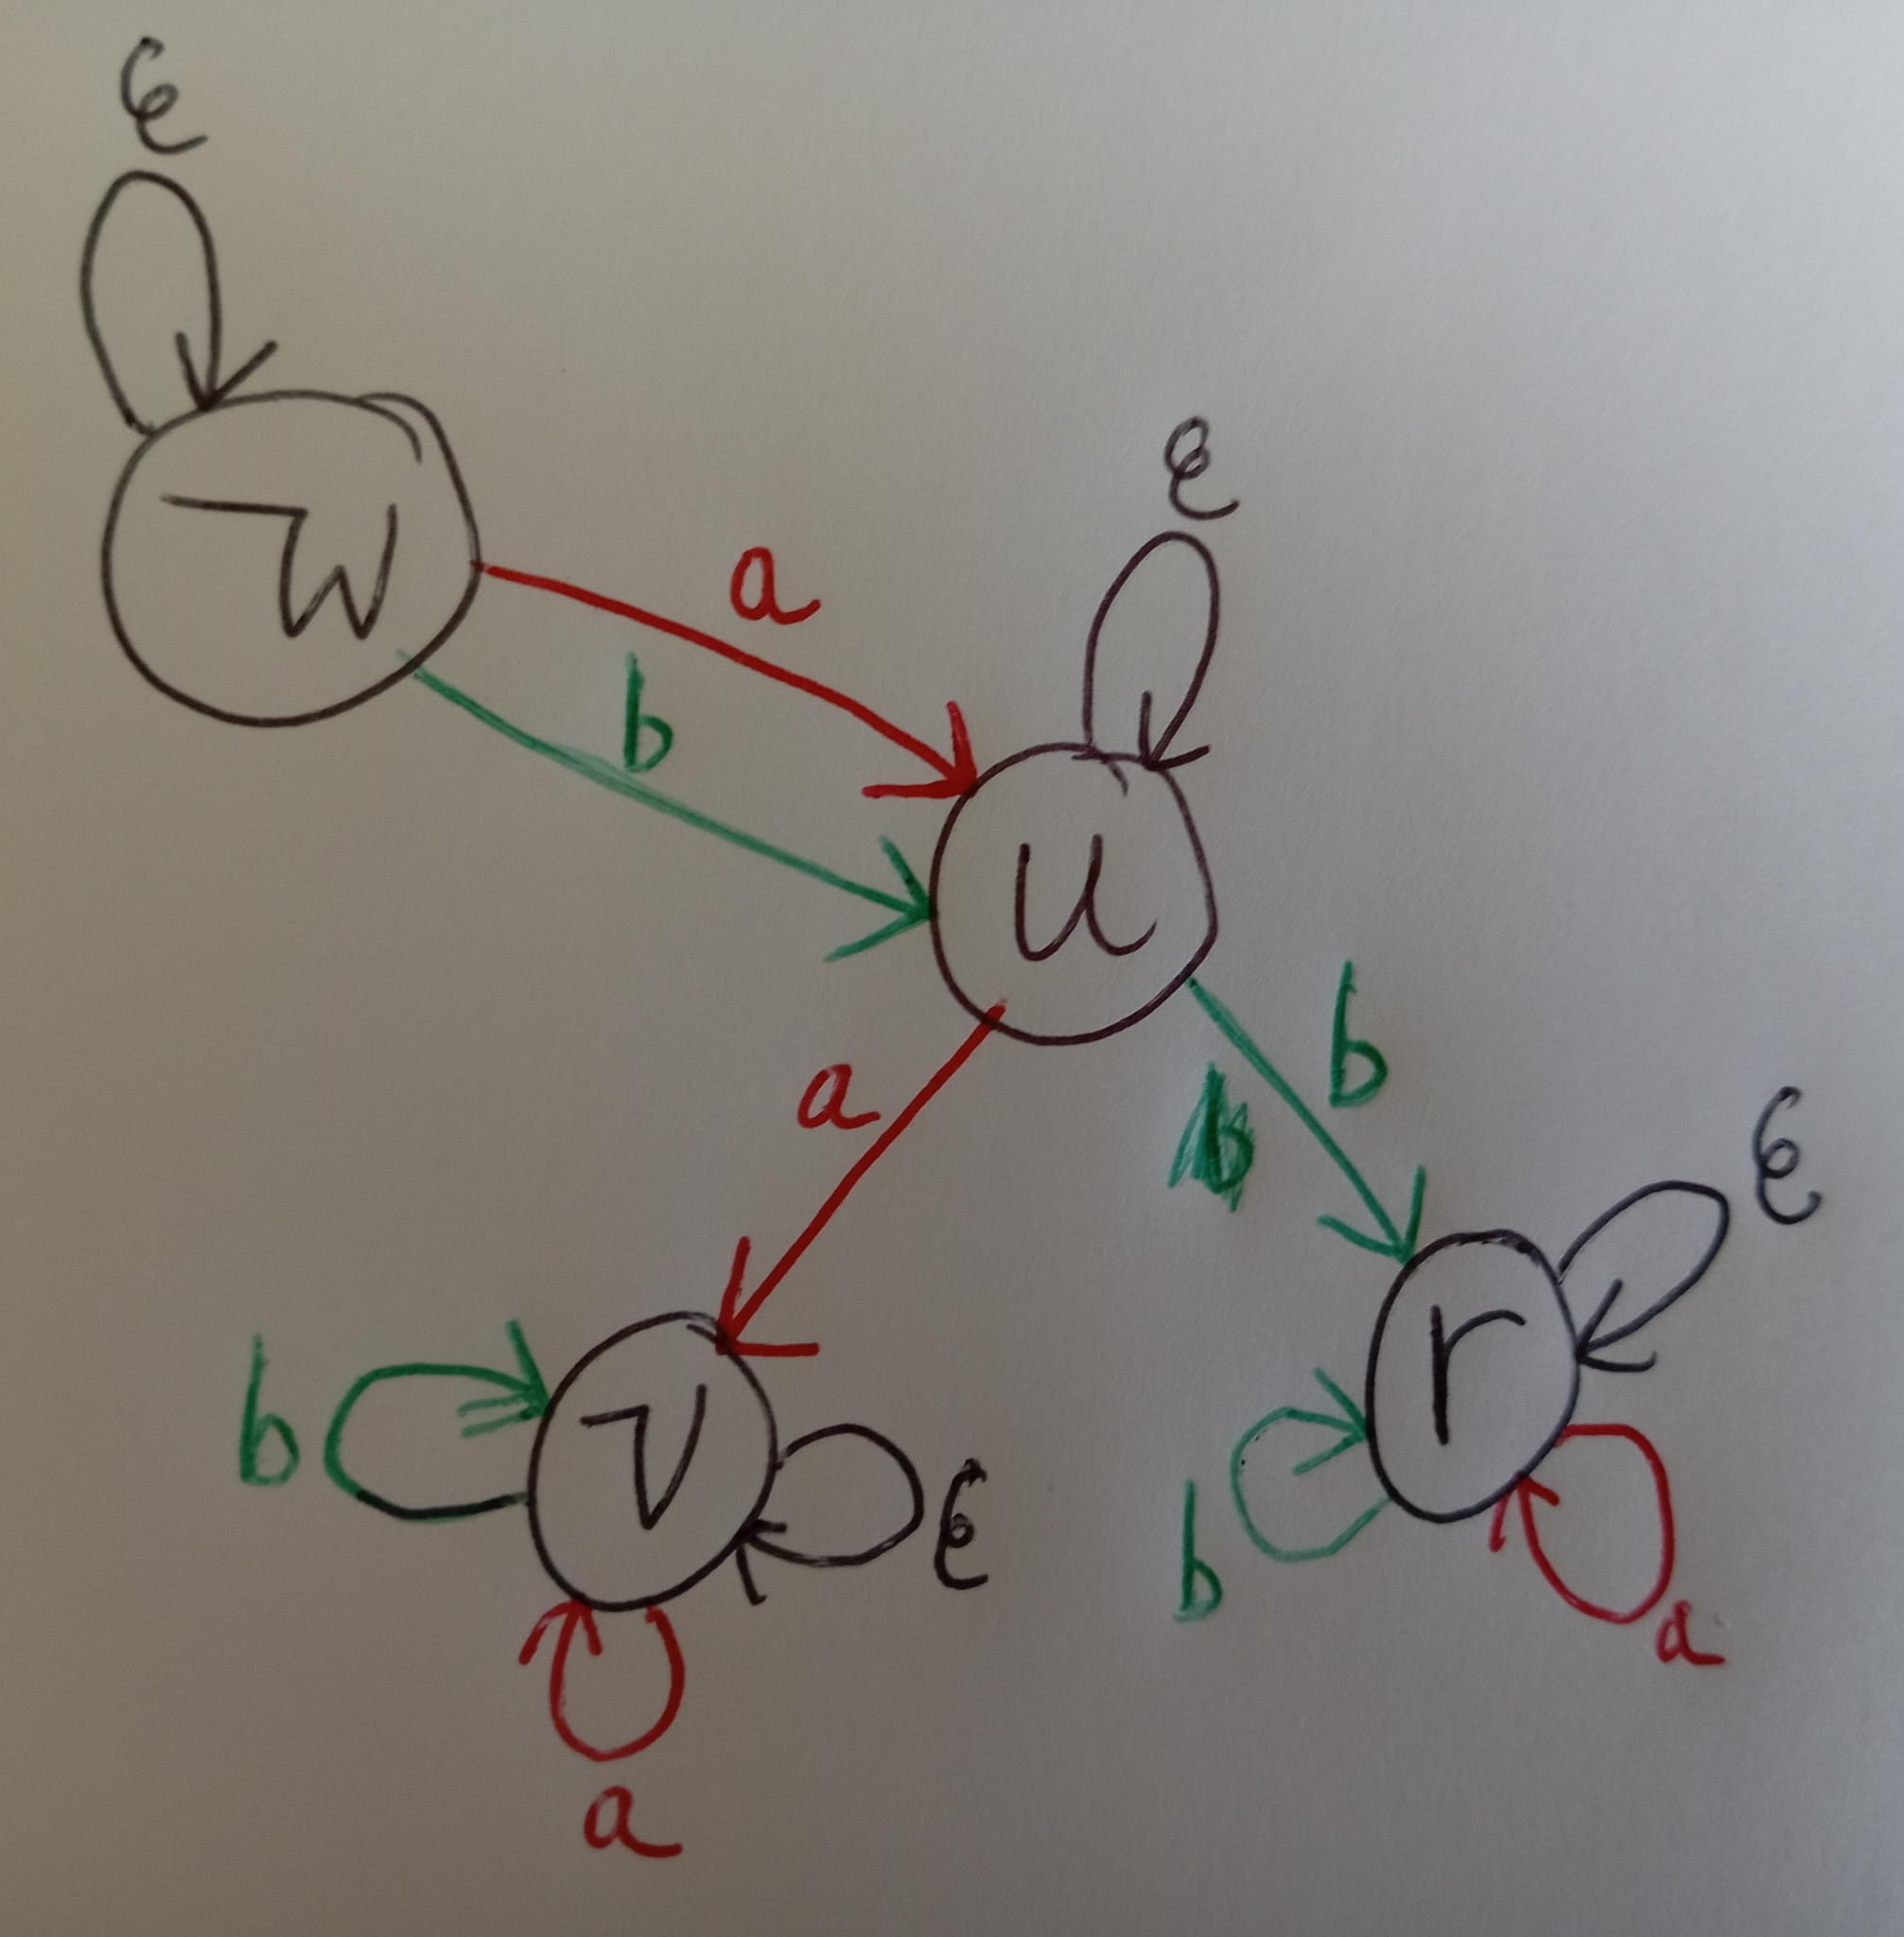
\includegraphics[width=0.5\linewidth]{6BeyondSBDRLLocalAlgebras/Images/local_equiv_classes_can_split_when_action_performed.jpeg}
    \caption{
    \draftnote{blue}{Caption}{}
    }
\end{figure}
Here we can see that $a \sim_{w} b$, but $a \not\sim_{u} b$.
Therefore, the $[a]_{\sim_{w}}$ equivalence class splits when $\xi_{(w, u)}$ is applied.
}



\begin{propositionE}
    $\circ_{\sim_{w}}$ is well-defined for $w \in W$ $\implies$ $\circ_{\sim_{u}}$ is well-defined for all $u \in W^{\hat{A}\to}$.
    \draftnote{blue}{To do}{
    Does this mean that $\circ_{\sim_{w}}$ being well-defined implies action-homogenous from $w$? No !
    }
    \draftnote{blue}{Consider}{Split into own prop: the part about local equivalence classes not splitting when $\circ_{\sim_{w}}$ is well-defined.}
\end{propositionE}
\begin{proofE}
\draftnote{blue}{Check this.}{}
\begin{enumerate}
    \item \textbf{Setup.}
    From \cref{prp:circ_sim_w_is_well_defined_iff_global_sim_coincides_with_local_sim}, we have
    \begin{equation}
        \text{$\circ_{\sim_{w}}$ is well-defined} \iff (\hat{A}^{*}/\sim)_{w} = \hat{A}^{*}/\sim_{w}
    \end{equation}
    Therefore, if we show that
    \begin{equation}
        \hat{A}^{*}/\sim_{w} = (\hat{A}^{*}/\sim)_{w} \implies \hat{A}^{*}/\sim_{u} = (\hat{A}^{*}/\sim)_{u} \quad \text{for all $u \in W^{\hat{A}\to}(w)$},
    \end{equation}
    we have that $\circ_{\sim_{u}}$ is well-defined for all $u \in W^{\hat{A}\to}(w)$.

    \item \textbf{Local equivalence classes don't split.}
    Consider two arbitrary actions $a,b \in \hat{A}^{*}$ such that
    \begin{equation}
        a \sim_{w} b
    \end{equation}
    From \cref{lem:local_and_global_quotients_effect},
    \begin{equation}
    \begin{aligned}
        & \hat{A}^{*}/\sim_{w} = (\hat{A}^{*}/\sim)_{w} \\
        \implies [ & a \sim_{w} a' 
        \\ & \iff \text{ for all $w' \in W^{\hat{A}\to}(w)$}: a \ast w' = a' \ast w'] \text{ for all $a,a' \in \hat{A}^{*}$}
    \end{aligned}
    \end{equation}
    Therefore, we have
    \begin{align}
        & a \sim_{w} b \\
        \implies & a \ast u = b \ast u \\
        \implies & a \sim_{u} b
    \end{align}
    where $u$ is an arbitrary world state in $W^{\hat{A}\to}(w)$.
    Therefore, when $\circ_{\sim_{w}}$ is well-defined, the partition of $\hat{A}^{*}$ by $\sim_{w}$ is preserved when passing to $\sim_{u}$.

    \item \textbf{If local equivalence classes merge, then their associated restricted global equivalence classes merge.}
    We have
    \begin{equation}
        a \sim_{w} b \implies a \sim_{u} b \quad \text{for all $a,a' \in \hat{A}^{*}$}
    \end{equation}
    In other words, if $\circ_{\sim_{w}}$ is well-defined the elements of local equivalence classes are not split under the map:
    \begin{align}
        & \xi_{(w, u)}: \mathscr{W}^{\hat{A}\to}(w) \to \mathscr{W}^{\hat{A}\to}(u) \\
        & \xi_{(w, u)}(\hat{A}^{*}/\sim_{w}) = \hat{A}^{*}/\sim_{u} \\
        & \xi_{(w, u)}((\hat{A}^{*}/\sim)_{w}) = (\hat{A}^{*}/\sim)_{u} \\
        & \xi_{(w, u)}: (w^{*}=w) \mapsto (w^{*}=u)
    \end{align}

    From \cref{prp:local_class_is_disjoint_union_of_global_classes},
    \begin{equation}
        [a]_{\sim_{w}} = \bigsqcup_{i \in I}[a_{i}]_{\sim}
    \end{equation}
    Since $\circ_{\sim_{w}}$ is well-defined, each local equivalence class consists of a single restricted global equivalence class\footnote{
    \draftnote{blue}{To do}{prove this separately ?}
    }:
    \begin{align}
        & [a_{1}]_{\sim_{w}} = ([a_{1}]_{\sim})_{w} \\
        & \vdots \\
        & [a_{j}]_{\sim_{w}} = ([a_{j}]_{\sim})_{w} \\
        & \vdots \\
        & [a_{n}]_{\sim_{w}} = ([a_{n}]_{\sim})_{w}
    \end{align}
    where $n = |\hat{A}^{*}/\sim_{w}|$.

    Since all the elements of $([a_{j}]_{\sim})_{w}$ are also elements of $[a_{j}]_{\sim_{w}}$, if
    \begin{equation}
        \xi_{(w, u)}([a_{j}]_{\sim_{w}}) = \xi_{(w, u)}([a_{k}]_{\sim_{w}})
    \end{equation}
    (i.e., if two local equivalence classes merge under the operation $\xi_{(w, u)}$), then all the elements of their associated restricted global equivalence classes will be members of the new merged local equivalence class:
    \begin{align}
        & \xi_{(w, u)}([a_{j}]_{\sim_{w}}) = \xi_{(w, u)}([a_{k}]_{\sim_{w}}) \\
        \implies & ([a_{j}]_{\sim})_{w} \in \xi_{(w, u)}([a_{j}]_{\sim_{w}}) \text{ and } ([a_{k}]_{\sim})_{w} \in \xi_{(w, u)}([a_{j}]_{\sim_{w}})
    \end{align}
    
    \begin{align}
        & \xi_{(w, u)}([a_{j}]_{\sim_{w}}) = \xi_{(w, u)}([a_{k}]_{\sim_{w}}) \\
        \implies & ([a_{j}]_{\sim})_{w} \in \xi_{(w, u)}([a_{j}]_{\sim_{w}}) \\
             & \text{and } ([a_{k}]_{\sim})_{w} \in \xi_{(w, u)}([a_{j}]_{\sim_{w}})
    \end{align}
    Therefore,
    \begin{equation}
        |\hat{A}^{*}/\sim_{u}| = |\hat{A}^{*}/\sim_{w}|
    \end{equation}
    and so, from \cref{prp:local_class_is_disjoint_union_of_global_classes},
    \begin{align}
        & |\hat{A}^{*}/\sim_{u}| = |\hat{A}^{*}/\sim_{u}| \\
        \implies & \hat{A}^{*}/\sim_{u} = \hat{A}^{*}/\sim_{u}
    \end{align}
    Since $u$ is an arbitrary world state in $W^{\hat{A}\to}(w)$, we have
    \begin{equation}
        \hat{A}^{*}/\sim_{u} = \hat{A}^{*}/\sim_{u} \quad \text{for all $u \in W^{\hat{A}\to}(w)$}
    \end{equation}

    \item \textbf{Show $\circ_{\sim_{u}}$ is well-defined for all $u \in W^{\hat{A}}(w)$.}
    From \cref{prp:circ_sim_w_is_well_defined_iff_global_sim_coincides_with_local_sim}, we have\footnote{
    Note that this does not mean that $\hat{A}^{*}/\sim_{w} = \hat{A}^{*}/\sim_{u}$ for all $u \in W^{\hat{A}\to}(w)$.
    Consider the world:
    \begin{figure}[H]
        % \centering
        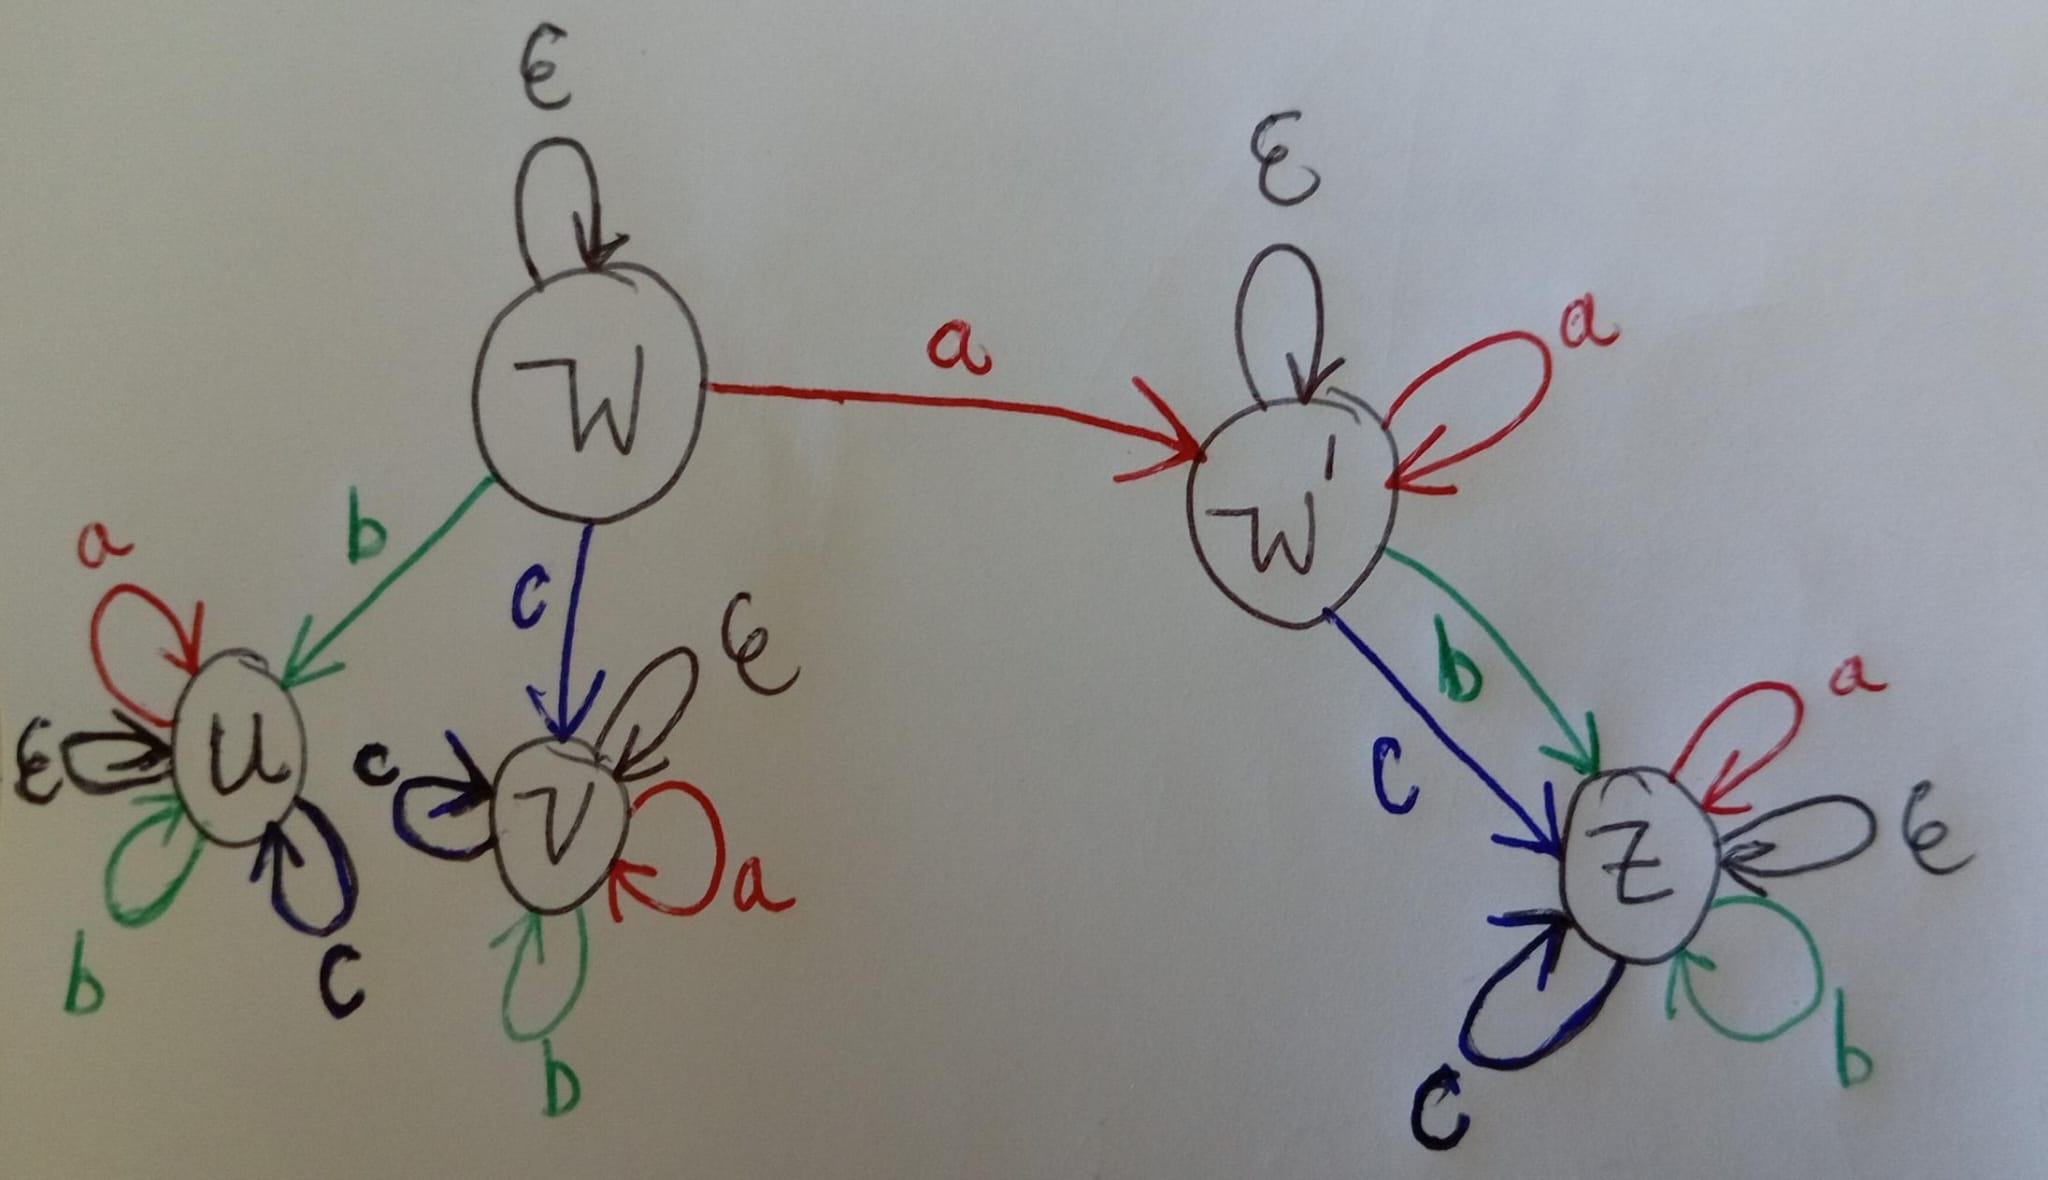
\includegraphics[width=0.5\linewidth]{6BeyondSBDRLLocalAlgebras/Images/circ_sim_w_defined_does_not_mean_algebra_is_constant.jpeg}
        \caption{\draftnote{blue}{To do}{}}
    \end{figure}
    In this world we have
    \begin{equation}
        (\hat{A}^{*}/\sim)_{w} = \hat{A}^{*}/\sim_{w} = \{ [\epsilon], [a], [b], [c], [ba] \},
    \end{equation}
    but
    \begin{equation}
        (\hat{A}^{*}/\sim)_{w'} = \hat{A}^{*}/\sim_{w'} = \{ [\epsilon], [b] \}.
    \end{equation}
    \draftnote{blue}{Consider}{
    NB: this world is not action-homogeneous.
    }
    }
    \begin{equation}
        (\hat{A}^{*}/\sim)_{u} = \hat{A}^{*}/\sim_{u} \iff \text{$\circ_{\sim_{u}}$ is well-defined}
    \end{equation}
    Since $u$ is an arbitrary world state in $W^{\hat{A}}(w)$, we have
    \begin{equation}
        \text{$\circ_{\sim_{u}}$ is well-defined}
    \end{equation}
    for all $u \in W^{\hat{A}}(w)$
\end{enumerate}
\end{proofE}

\draftnote{blue}{Consider}{
Does the number of unique Cayley table constructions monotonically decreases (monotonically non-increasing) (i.e., $\circ_{\sim_{w}}$ becomes "more well-defined") as actions are performed ?
No because $\sim_{w}$ classes can split unless $\circ_{\sim_{w}}$ is well-defined ?
}

\begin{propositionE}\label{prp:circ_sim_w_not_well_defined_does_not_mean_no_associativity}
    $\circ_{\sim_{w}}$ is not well-defined on $\hat{A}^{*}/\sim_{w}$ $\centernot\implies$ there exists a Cayley table construction of $(\hat{A}^{*}/\sim_{w}, \circ_{\sim_{w}})$ that does not satisfy the associativity property.
\end{propositionE}
\begin{proofE}
\draftnote{blue}{To do}{
Note about how $\bot$ could be replaced by a non undefined state with the same absorbing properties.
}
\textbf{Proof by example.}
\begin{enumerate}
    \item \textbf{Set up.}
    \draftnote{blue}{To do}{Give this world a Greek letter.}
    Consider a world-agent pair $\mathscr{W}-\mathscr{A}$ with $W = \{ w, w_{1}, w_{2}, \bot \}$, $\hat{A} = \{\hat{a}, \hat{b}\}$, and $\hat{\ast}$ given by
    \footnote{\begin{figure}[H]
        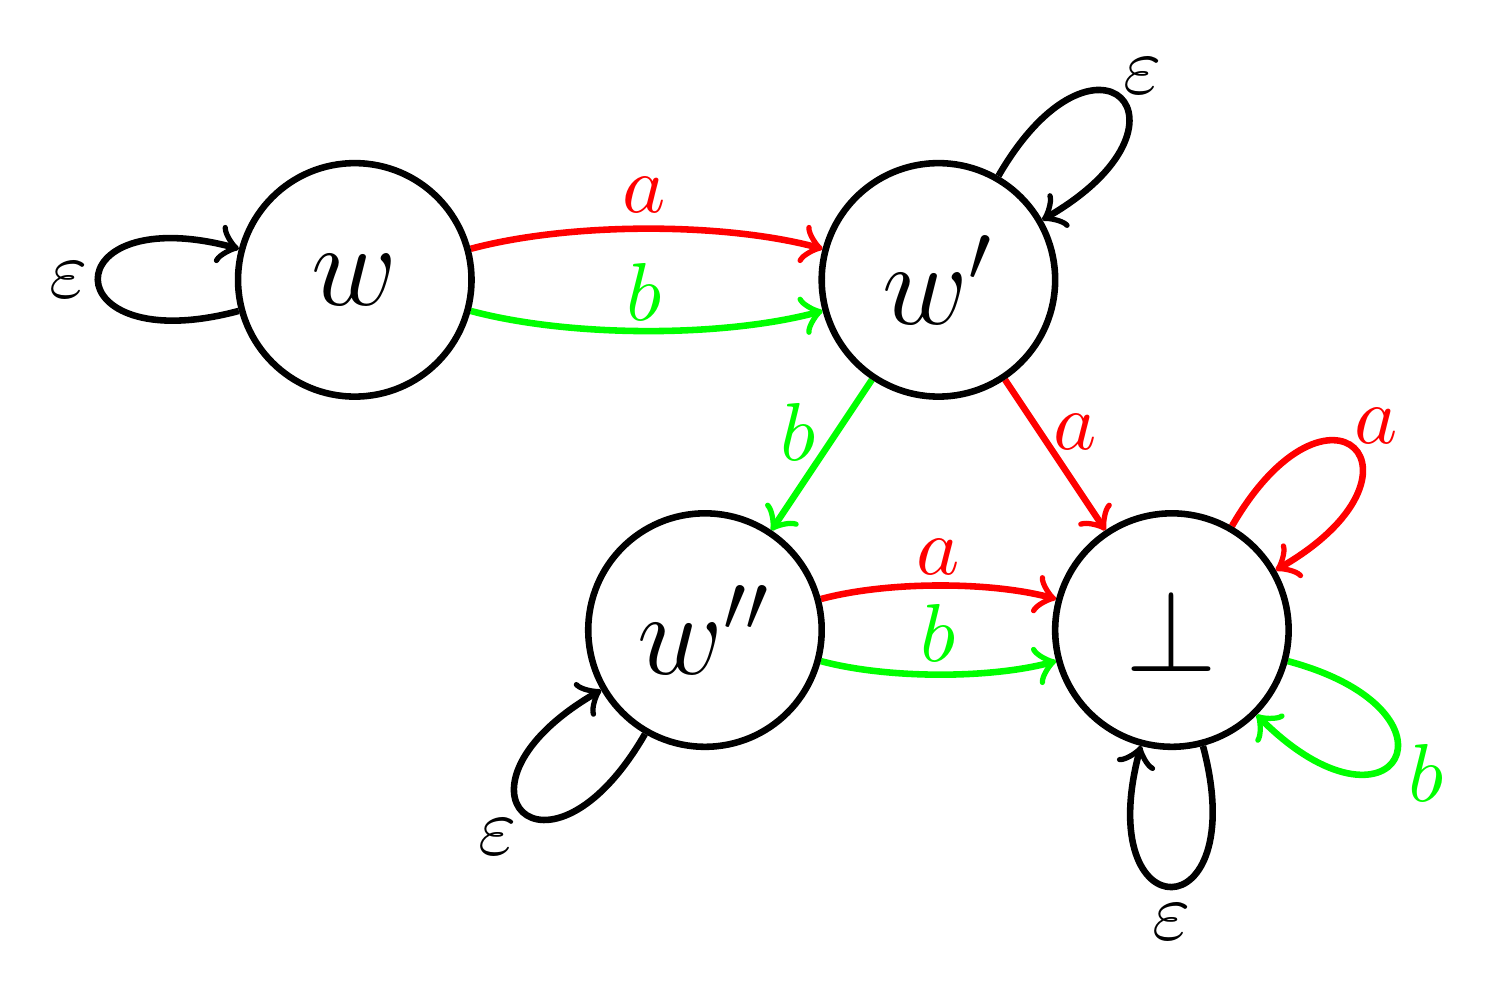
\includegraphics[width=0.5\linewidth]{6BeyondSBDRLLocalAlgebras/Images/circ_sim_w_not_well_defined_does_not_mean_no_associativity_counter_example.png}
        \caption{
        \draftnote{blue}{To do}{Improve caption.}
        }
    \end{figure}}
    \begin{table}[H]
        \centering
        \begin{tabular}{c|cccc}
            $\hat{\ast}$   & $w$       & $w_{1}$   & $w_{2}$   & $\bot$ \\
            \hline
            $\epsilon$      & $w$       & $w_{1}$   & $w_{2}$   & $\bot$ \\
            $\hat{a}$       & $w_{1}$   & $\bot$   & $\bot$   & $\bot$ \\
            $\hat{b}$       & $w_{1}$   & $w_{2}$   & $\bot$   & $\bot$
        \end{tabular}
        \caption{
        \draftnote{blue}{To do}{Improve caption.}
        }
    \end{table}

    \item \textbf{Show $\circ_{\sim_{w}}$ not well-defined.}
    From $\hat{\ast}$ we can see that
    \begin{equation}
        [a]_{\sim_{w}} = [b]_{\sim_{w}}
    \end{equation}
    Testing the well-definedness of $\circ_{\sim}$ using $[a]_{\sim_{w}} = [b]_{\sim_{w}}$ and $[a]_{\sim_{w}} = [a]_{\sim_{w}}$ gives
    \begin{align}
        & (b \circ a) \ast w = b \ast (a \ast w) = b \ast w_{1} = w_{2} \\
        & (a \circ a) \ast w = a \ast (a \ast w) = a \ast w_{1} = \bot \\
        \implies & [b \circ a]_{\sim_{w}} \neq [a \circ a]_{\sim_{w}} \\
        \implies & \circ_{\sim_{w}} \; \text{not well defined}
    \end{align}

    \item \textbf{Number of unique Cayley table constructions.}
    Using our algorithms described in \draftnote{blue}{To do}{[sections ????]}, we generate the elements of $(\hat{A}^{*}/\sim)_{w}$ and $\hat{A}^{*}/\sim_{w}$ for our example:
    \begin{align}
        & (\hat{A}^{*}/\sim)_{w} = \{ [\epsilon]_{\sim}, [a]_{\sim}, [b]_{\sim}, [aa]_{\sim}, [ba]_{\sim} \} \\
        & \hat{A}^{*}/\sim_{w} = \{ [\epsilon]_{\sim_{w}}, [a]_{\sim_{w}}, [aa]_{\sim_{w}}, [ba]_{\sim_{w}} \}
    \end{align}
    We have the following equivalence classes of $\hat{A}^{*}$ under $\sim_{w}$:
    \begin{align}
        & [\epsilon]_{\sim_{w}} = \{ \epsilon \} \quad (w \mapsto w) \\
        & [a]_{\sim_{w}} = \{ a, b \} \quad (w \mapsto w_{1}) \\
        & [ba]_{\sim_{w}} = \{ ba, bb \} \quad (w \mapsto w_{2}) \\
        & [aa]_{\sim_{w}} = \{ aa, bbb, abb \} \\
        & \cup \{ \text{any sequence suffixed with $aa$, $bbb$, or $abb$} \} \quad (w \mapsto \bot)
    \end{align}
    We've not included sequences containing $\epsilon$ composed with minimum actions explicitly in our equivalence classes since these sequences are not relevant to our analysis because $\epsilon$ always returns the world state it is applied on (i.e., $[\epsilon \circ x]_{\sim_{w}} = [x]_{\sim_{w}}$ and $[x \circ \epsilon]_{\sim_{w}} = [x]_{\sim_{w}}$ for all $x \in \hat{A}^{*}$).

    We can use \cref{prp:num_unique_cayley_table_constructions_is_product} to calculate the number $|\mathcal{C}|$ of unique Cayley table constructions of $(\hat{A}^{*}/\sim_{w}, \circ_{\sim_{w}})$:
    \begin{equation}
        |\mathcal{C}| = \prod_{j \in J} m_{j} = (1)(2)(1)(1) = 2
    \end{equation}

    \item \textbf{Find unique Cayley table constructions.}
    The local equivalence class $[a]_{\sim_{w}} \in \hat{A}^{*}/\sim_{w}$ is the only local equivalence class that contains more than one global equivalence class in $(\hat{A}^{*}/\sim)_{w}$.
    This means both unique Cayley table constructions will be generated by changing the representative element of $[a]_{\sim_{w}}$ to be representative elements of each of the global equivalence classes in $[a]_{\sim_{w}}$.

    Let $T([a]_{\sim})$ be the Cayley table construction that uses $a$ as the representative element of $[a]_{\sim_{w}}$, and let $T([b]_{\sim})$ be the Cayley table construction that uses $b$ as the representative element of $[a]_{\sim_{w}}$.
    \begin{table}[H]
        \centering
        \begin{tabular}{c|cccc}
            $\circ_{\sim_{w}}$              & $[\epsilon]_{\sim_{w}}$     & $\bm{[a]_{\sim_{w}}}$   & $[aa]_{\sim_{w}}$   & $[ba]_{\sim_{w}}$ \\
            \hline
            $[\epsilon]_{\sim_{w}}$        & $[\epsilon]_{\sim_{w}}$      & $\bm{[a]_{\sim_{w}}}$    & $[aa]_{\sim_{w}}$   & $[ba]_{\sim_{w}}$ \\
            $\bm{[a]_{\sim_{w}}}$          & $\bm{[a]_{\sim_{w}}}$        & $\bm{[aa]_{\sim_{w}}}$   & $[aa]_{\sim_{w}}$   & $[aa]_{\sim_{w}}$ \\
            $[aa]_{\sim_{w}}$              & $[aa]_{\sim_{w}}$            & $[aa]_{\sim_{w}}$   & $[aa]_{\sim_{w}}$   & $[aa]_{\sim_{w}}$ \\
            $[ba]_{\sim_{w}}$              & $[ba]_{\sim_{w}}$            & $[aa]_{\sim_{w}}$   & $[aa]_{\sim_{w}}$   & $[aa]_{\sim_{w}}$ \\
        \end{tabular}
        \caption{
        $T([a]_{\sim})$.
        \draftnote{blue}{To do}{Improve caption.}
        }
    \end{table}
    \begin{table}[H]
        \centering
        \begin{tabular}{c|cccc}
            $\circ_{\sim_{w}}$              & $[\epsilon]_{\sim_{w}}$     & $\bm{[b]_{\sim_{w}}}$   & $[aa]_{\sim_{w}}$   & $[ba]_{\sim_{w}}$ \\
            \hline
            $[\epsilon]_{\sim_{w}}$        & $[\epsilon]_{\sim_{w}}$      & $\bm{[b]_{\sim_{w}}}$    & $[aa]_{\sim_{w}}$   & $[ba]_{\sim_{w}}$ \\
            $\bm{[b]_{\sim_{w}}}$          & $\bm{[b]_{\sim_{w}}}$        & $\bm{[ba]_{\sim_{w}}}$ & $[aa]_{\sim_{w}}$ & $[aa]_{\sim_{w}}$ \\
            $[aa]_{\sim_{w}}$              & $[aa]_{\sim_{w}}$            & $[aa]_{\sim_{w}}$   & $[aa]_{\sim_{w}}$   & $[aa]_{\sim_{w}}$ \\
            $[ba]_{\sim_{w}}$              & $[ba]_{\sim_{w}}$            & $[aa]_{\sim_{w}}$   & $[aa]_{\sim_{w}}$   & $[aa]_{\sim_{w}}$ \\
        \end{tabular}
        \caption{
        $T([b]_{\sim})$.
        \draftnote{blue}{To do}{Improve caption.}
        }
    \end{table}
    
    \item \textbf{Properties of the unique Cayley table constructions.}
    \begin{table}[H]
        \centering
        \begin{tabular}{l|c}
        \textbf{Property} & \textbf{Present?} \\
        \hline
        Associative & Y \\
        Identity & Y \\
        Inverses & N \\
        \hline
        Commutative & Y \\
        \end{tabular}
        \caption{
        Properties of $T([a]_{\sim})$.
        \draftnote{blue}{To do}{Sort table formatting.}
        }
    \end{table}
    
    \begin{table}[H]
        \centering
        \begin{tabular}{l|c}
        \textbf{Property} & \textbf{Present?} \\
        \hline
        Associative & Y \\
        Identity & Y \\
        Inverses & N \\
        \hline
        Commutative & Y \\
        \end{tabular}
        \caption{
        Properties of $T([b]_{\sim})$.
        \draftnote{blue}{To do}{Sort table formatting.}
        \draftnote{blue}{To do}{Check this algorithmically.}
        }
    \end{table}

    \item \textbf{Conclusion.}
    Since $T([a]_{\sim})$ and $T([b]_{\sim})$ both satisfy the associativity property, every unique Cayley table construction of $(\hat{A}^{*}/\sim_{w}, \circ_{\sim_{w}})$ for our example world satisfies the associativity property.
\end{enumerate}
\end{proofE}


\draftnote{blue}{To do}{
Code to calculate the number of unique Cayley table constructions and then to generate them.
\textbf{To calculate:}
\begin{enumerate}
    \item Generate $\hat{A}^{*}/\sim_{w}$ and $(\hat{A}^{*}/\sim)_{w}$.
    \item Work out which local equivalence class of $\hat{A}^{*}/\sim_{w}$ that each element of $(\hat{A}^{*}/\sim)_{w}$ is in.
    \item Find product.
\end{enumerate}
\textbf{To generate:}
\begin{enumerate}
    \item Generate $\hat{A}^{*}/\sim_{w}$ and $(\hat{A}^{*}/\sim)_{w}$.
    \item Work out which local equivalence class of $\hat{A}^{*}/\sim_{w}$ that each element of $(\hat{A}^{*}/\sim)_{w}$ is in.
    \item Generate all distinct global-class choices.
    \item Generate Cayley table constructions.
\end{enumerate}
}

\begin{propositionE}
    A Cayley table construction of $(\hat{A}^{*}/\sim_{w}, \circ_{\sim_{w}})$ satisfies the associativity property $\centernot\implies$ $\circ_{\sim_{w}}$ is well-defined.
\end{propositionE}
\begin{proofE}
    Proof by example using the same example world as given in \cref{prp:circ_sim_w_not_well_defined_does_not_mean_no_associativity}, which is a world where $\circ_{\sim_{w}}$ is not well-defined and the associativity property is satisfied by a Cayley table construction of $(\hat{A}^{*}/\sim_{w}, \circ_{\sim_{w}})$.
\end{proofE}

%%%%%%%%%%%%%%%%%%%%%%%%%%%%%%
\subsection{
Proofs about $[\epsilon]_{\sim_{w}}$
}

\begin{propositionE}
    $\circ_{\sim_{w}}$ is well-defined on $\hat{A}^{*}/\sim_{w}$ $\implies$ $[\epsilon]_{\sim_{w}}$ is the identity element of $(\hat{A}^{*}/\sim_{w}, \circ_{\sim_{w}})$.
    \draftnote{blue}{To do}{
    $[\epsilon]_{\sim}$ is also the identity element of $((\hat{A}^{*}/\sim)_{w}, \circ_{\sim_{w}})$.
    }
\end{propositionE}
\begin{proofE}
\begin{enumerate}
    \item \textbf{Well-definedness.}
    If $\circ_{\sim_{w}}$ is well-defined, then for any $a, a' \in [a]_{\sim_{w}}$ and $b, b' \in [b]_{\sim_{w}}$,
    \begin{equation}
        [a]_{\sim_{w}} \circ_{\sim_{w}} [b]_{\sim_{w}} = [a \circ b]_{\sim_{w}} = [a' \circ b']_{\sim_{w}}
    \end{equation}
    by definition; this means that composition of equivalence classes under $\circ_{\sim_{w}}$ is independent of the choice of representation.

    \item \textbf{$\epsilon$ is identity element.}
    By the definition of $\epsilon \in \hat{A}^{*}$,
    \begin{equation}
        \epsilon \ast w' = w' \quad \text{for all $w' \in W$}
    \end{equation}
    For any $a \in \hat{A}^{*}$,
    \begin{align}
        & [\epsilon]_{\sim_{w}} \circ_{\sim_{w}} [a]_{\sim_{w}} = [\epsilon \circ a]_{\sim_{w}} = [a]_{\sim_{w}} \\
        & [a]_{\sim_{w}} \circ_{\sim_{w}} [\epsilon]_{\sim_{w}} = [\epsilon \circ a]_{\sim_{w}} = [a]_{\sim_{w}}
    \end{align}
    Therefore, $[\epsilon]_{\sim_{w}}$ is the identity element of $(\hat{A}^{*}/\sim_{w}, \circ_{\sim_{w}})$.
\end{enumerate}
\end{proofE}


\begin{propositionE}
    The Cayley table constructions of $(\hat{A}^{*}/\sim_{w}, \circ_{\sim_{w}})$ do not always satisfy the identity property.
\end{propositionE}
\begin{proofE}
\textbf{Proof by example.}
\begin{enumerate}
    \item \textbf{Set up.}
        \draftnote{blue}{To do}{Give this world a Greek letter.}
        Consider a world-agent pair $\mathscr{W}-\mathscr{A}$ with $W = \{ w, w', w'', \bot \}$, $\hat{A} = \{a, b\}$, and $\hat{\ast}$ given by\footnote{
        \begin{figure}[H]
            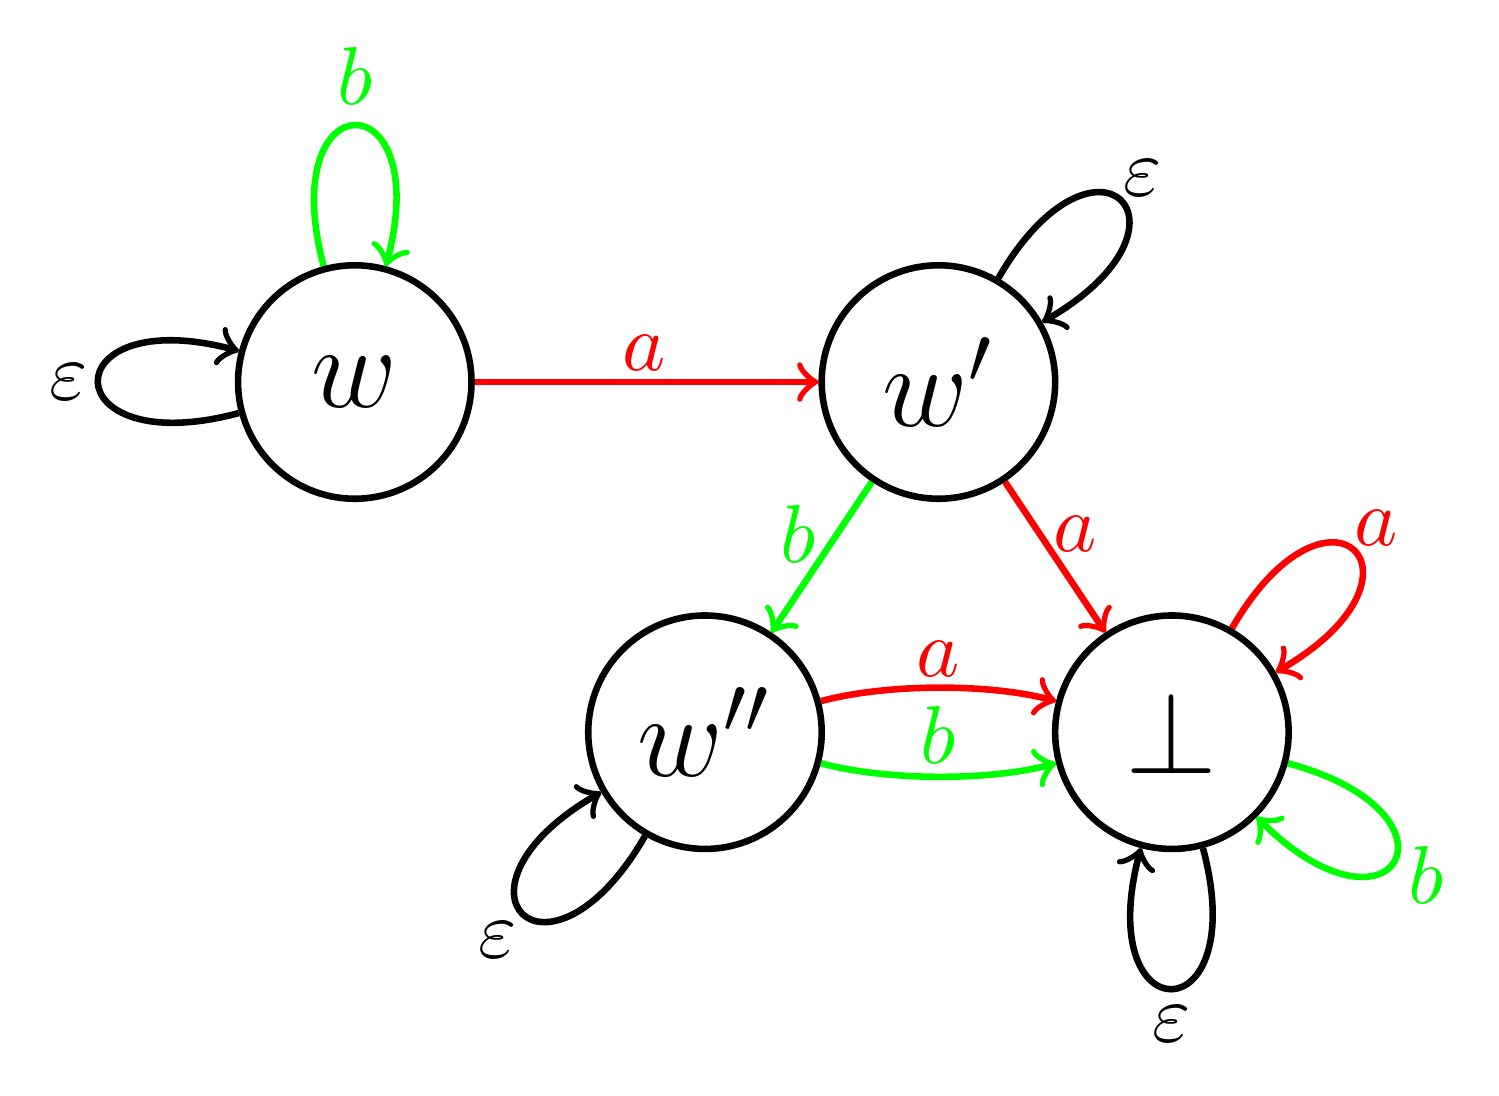
\includegraphics[width=0.5\linewidth]{6BeyondSBDRLLocalAlgebras/Images/cayley_table_constructions_dont_always_satisfy_identity.png}
            \caption{Caption}
        \end{figure}
        }
        \begin{table}[H]
            \centering
            \begin{tabular}{c|cccc}
                $\hat{\ast}$   & $w$       & $w'$      & $w''$     & $\bot$ \\
                \hline
                $\epsilon$      & $w$       & $w'$      & $w''$     & $\bot$ \\
                $a$             & $w'$      & $\bot$    & $\bot$    & $\bot$ \\
                $b$             & $w$       & $w''$     & $\bot$    & $\bot$
            \end{tabular}
            \caption{
            \draftnote{blue}{To do}{Improve caption.}
            }
        \end{table}
    \item \textbf{Construct Cayley table with no identity.}
    We will now construct a Cayley table for $(\hat{A}^{*}/\sim_{w}, \circ_{\sim_{w}})$ that does not satisfy the identity property.
    We choose to use $b \in \hat{A}^{*}$ as the representative element for $[\epsilon]_{\sim_{w}}$.
    \begin{table}[H]
        \centering
        \begin{tabular}{c|cccc}
            $\circ_{\sim_{w}}$  & $[b]_{\sim_{w}}$  & $[a]_{\sim_{w}}$   & $[ba]_{\sim_{w}}$  & $[aa]_{\sim_{w}}$ \\
            \hline
            $[b]_{\sim_{w}}$    & $[b]_{\sim_{w}}$  & $[ba]_{\sim_{w}}$  & $[aa]_{\sim_{w}}$  & $[aa]_{\sim_{w}}$ \\
            $[a]_{\sim_{w}}$    & $[a]_{\sim_{w}}$  & $[aa]_{\sim_{w}}$  & $[aa]_{\sim_{w}}$  & $[aa]_{\sim_{w}}$ \\
            $[ba]_{\sim_{w}}$   & $[ba]_{\sim_{w}}$ & $[aa]_{\sim_{w}}$  & $[aa]_{\sim_{w}}$  & $[aa]_{\sim_{w}}$ \\
            $[aa]_{\sim_{w}}$   & $[aa]_{\sim_{w}}$ & $[aa]_{\sim_{w}}$  & $[aa]_{\sim_{w}}$  & $[aa]_{\sim_{w}}$
        \end{tabular}
        \caption{
        \draftnote{blue}{To do}{Improve caption.}
        }
    \end{table}
    From inspecting the Cayley table construction we can see it does not satisfy the identity property.\footnote{
    In fact, any world where there is some action $a \in \hat{A}^{*}$ that satisfies
    \begin{equation}
        [a]_{\sim_{w}} = [\epsilon]_{\sim} \quad \text{but} \; [a]_{\sim} \neq [\epsilon]_{\sim}
    \end{equation}
    will have at least one Cayley table construction that does not satisfy the identity property.
    This follows from the contrapositive of \cref{prp:cayley_table_construction_satisfies_identity_iff_element_of_global_epsilon_used_as_representative}.
    }
\end{enumerate}
\end{proofE}


\begin{propositionE}\label{prp:cayley_table_construction_satisfies_identity_iff_element_of_global_epsilon_used_as_representative}
    A cayley table construction of $(\hat{A}^{*}/\sim_{w}, \circ_{\sim_{w}})$ satisfies the identity property $\iff$ an element of $[\epsilon]_{\sim} \in (\hat{A}^{*}/\sim)_{w}$ is used as the representative of $[\epsilon]_{\sim_{w}}$ in the Cayley table construction of $(\hat{A}^{*}/\sim_{w}, \circ_{\sim_{w}})$.
\end{propositionE}
\begin{proofE}
\begin{enumerate}
    \item \textbf{Identity property $\implies$ representative is in $[\epsilon]_{\sim}$.}
    Assume that the Cayley table construction satisfied the identity property.
    Let $[e]_{\sim_{w}} \in \hat{A}^{*}/\sim_{w}$ be the identity element in the Cayley table construction and let $e \in \hat{A}^{*}$ be the representative of $[e]_{\sim_{w}}$ in the Cayley table construction.
    By definition of identity, $[e]_{\sim_{w}}$ satisfies
    \begin{align}
        & [a \circ e]_{\sim_{w}} = [a]_{\sim_{w}}  \quad \text{for all $a \in \hat{A}^{*}$} \label{eqn:identity_property_of_e_1} \\
        \text{and } & [e \circ a]_{\sim_{w}} = [a]_{\sim_{w}} \quad \text{for all $a \in \hat{A}^{*}$} \label{eqn:identity_property_of_e_2}
    \end{align}
    We will use \cref{eqn:identity_property_of_e_1,eqn:identity_property_of_e_2} to derive conditions on the representative $e$.
    For \cref{eqn:identity_property_of_e_1}, we have
    \begin{align}
        & (a \circ e) \ast w = a \ast w \quad \text{for all $a \in \hat{A}^{*}$} \\
        \implies & a \ast (e \ast w) = a \ast w \quad \text{for all $a \in \hat{A}^{*}$} \\
        \implies & e \ast w = w \quad \text{for all $a \in \hat{A}^{*}$} \label{eqn:identity_condition_e_1}
    \end{align}
    
    For \cref{eqn:identity_property_of_e_2}, we have
    \begin{align}
        & (e \circ a) \ast w = a \ast w \quad \text{for all $a \in \hat{A}^{*}$} \\
        \implies & e \ast (a \ast w) = a \ast w \quad \text{for all $a \in \hat{A}^{*}$} \\
        \implies & e \ast w' = w' \quad \textit{where $a \ast w = w'$} \quad \text{for all $a \in \hat{A}^{*}$}
    \end{align}
    Since this must hold for all $a \in \hat{A}^{*}$, $w'$ can be any world state that is reachable from $w$ (i.e., $w' \in W^{\hat{A}\to}(w)$).
    This gives us\footnote{Note that this condition includes \cref{eqn:identity_condition_e_1}.}
    \begin{equation}\label{eqn:identity_condition_e_2}
        e \ast w' = w' \quad \text{for all $w' \in W^{\hat{A}\to}(w)$}
    \end{equation}
    Since $\epsilon$ satisfies $\epsilon \ast w = w$ for all $w \in W$, \cref{eqn:identity_condition_e_2} is the definition for $e$ being an element of $[\epsilon]_{\sim} \in (\hat{A}^{*}/\sim)_{w}$.
    
   \item \textbf{Identity property $\impliedby$ representative is in $[\epsilon]_{\sim}$.}
   Let the representative of $[\epsilon]_{\sim_{w}}$ be an element $e \in [\epsilon]_{\sim}$ where $[\epsilon]_{\sim} \in (\hat{A}^{*}/\sim)_{w}$.
   By definition of $[\epsilon]_{\sim} \in (\hat{A}^{*}/\sim)_{w}$, we have
   \begin{equation}
       e \ast w' = w' \quad \text{for all $w' \in W^{\hat{A}\to}(w)$}
   \end{equation}
   For any $[a]_{\sim_{w}} \in \hat{A}^{*}/\sim_{w}$, we have
   \begin{align}
       & (e \circ a) \ast w \\
       = & e \ast (a \ast w) \\
       = & e \ast w' \quad \text{where $w' = a \ast w$} \\
       = & w' \\
       = & a \ast w \\
       \implies & [a \circ e]_{\sim_{w}} = [a]_{\sim_{w}}
   \end{align}
   and
   \begin{align}
       & (a \circ e) \ast w \\
       = & a \ast (e \ast w) \\
       = & a \ast w \\
       \implies & [a \circ e]_{\sim_{w}} = [a]_{\sim_{w}}
   \end{align}
    Therefore $[e]_{\sim_{w}}$ satisfies the identity property.
\end{enumerate}
\end{proofE}

\begin{corollary}
    Any world where $[\epsilon]_{\sim_{w}}$ contains more than one of the global equivalence classes in $(\hat{A}^{*}/\sim)_{w}$, has at least one Cayley table construction of $(\hat{A}^{*}/\sim_{w}, \circ_{\sim_{w}})$ that does not satisfy the identity property.
\end{corollary}




\draftnote{blue}{To do}{
Show example using $\mathscr{W}_{\beta}$ with identity treatment of when switching the representative element leads to a different Cayley table construction.
}
\draftnote{blue}{Consider}{
Do elements of the identity class form a group in some way ?
}

%%%%%%%%%%%%%%%%%%%%%%%%%%%%%%%%%%%%%%%
\subsection{
What have we discovered ?
}
\draftnote{green}{To do}{
\begin{enumerate}
    \item Table summarising the associativity vs well-defined properties.
    \item Associativity breaking as an indicator that $\circ_{\sim_{w}}$ is not well-defined.
    \item We cannot guarantee that any of the group properties are satisfied or are not satisfied in a Cayley table construction of $(\hat{A}^{*}/\sim_{w}, \circ_{\sim_{w}})$. - these are pseudo algebras ?
    \item Need something about the potential issues with $(\hat{A}^{*}/\sim)_{w}$ when an agent is continual learning
    \begin{itemize}
        \item The structure of $(\hat{A}^{*}/\sim)_{w}$ can change as $\mathscr{W}^{\hat{A}\to}(w)$ changes.
        \item The structure of $(\hat{A}^{*}/\sim)_{w}$ won't change if the world is action homogeneous from $w$ (because $\mathscr{W}^{\hat{A}\to}(w') \cong \mathscr{W}^{\hat{A}\to}(w'')$ for all $w',w'' \in W^{\hat{A}\to}(w)$).
    \end{itemize}
\end{enumerate}
}

%%%%%%%%%%%%%%%%%%%%%%%%%%%%%%%%%%%%%%%
\section{
Worlds with uniform local algebraic structures
}

\draftnote{blue}{Include in intro}{
Point out that $\mathscr{W}_{\alpha}$ appears to have a very regular structure.
For example, the number of in-going and out-going transformations labelled by each action $a \in \hat{A}^{*}$ is the same for each world state.
}

What properties of the world $\mathscr{W}_{\alpha}$ mean that the local Cayley tables $T_{\sim_{w}}$ are not just isomorphic, but are identical for all $w \in W$?

$\mathscr{W}_{\alpha}$ has a uniform local algebraic structure across its states.


\begin{propositionE}
    \label{prp:all_local_cayley_tables_from_w_are_identical_means_local_cayley_table_conincides_with_global_algebra_from_w}
    \draftnote{blue}{To do}{Make this about reachable subworlds.}
    \draftnote{blue}{To do}{
    Can we prove this for when there are multiple constructions of the local Cayley table (i.e., if the set $\mathcal{C}$ of unique constructions of two local Cayley tables are the same then the two Cayley tables are equal) ?
    Need different notation for all Cayley table constructions vs single Cayley table construction.
    }
    $T_{\sim_{w}}(\hat{A}^{*}, \circ) = T_{\sim_{w'}}(\hat{A}^{*}, \circ)$ for all $w' \in W^{\hat{A}\to}(w)$ $\iff$ 
    $(\hat{A}^{*}/\sim)_{w} = \hat{A}^{*}/\sim_{w'}$ for all $w' \in W^{\hat{A}\to}(w)$.
    \draftnote{blue}{Put as footnote the first time we use this}{
    $\hat{A}^{*}/\sim_{w} = \hat{A}^{*}/\sim_{w'}$ means $\{ [x]_{\sim_{w}} \mid x \in \hat{A}^{*} \} = \{ [x]_{\sim_{w}} \mid x \in \hat{A}^{*} \}$ (i.e., $\sim_{w}$ and $\sim_{w'}$ identically partition $\hat{A}^{*}$ (not up to isomorphism).
    }
\end{propositionE}
\begin{proofE}
\begin{enumerate}
    \item \textbf{Forwards direction $\implies$.}
    Assume $T_{\sim_{w'}}(\hat{A}^{*}, \circ)$ for all $w \in W^{\hat{A}\to}(w)$.
    \begin{enumerate}
        \item \textbf{Equality of local Cayley tables $\implies$ equality of local equivalence classes.}
        For local Cayley tables $T_{\sim_{w'}}$ for all $w' \in W^{\hat{A}\to}(w)$ to be identical, the labels, which are the equivalence classes in $\hat{A}^{*}/\sim_{w'}$, and their compositions $[a]_{\sim_{w'}} \circ_{\sim_{w'}} [a']_{\sim_{w'}}$ must match.
        Therefore,
        \begin{align}
            & T_{\sim_{w}}(\hat{A}^{*}, \circ) = T_{\sim_{w'}}(\hat{A}^{*}, \circ) \quad \text{for all $w' \in W^{\hat{A}\to}(w)$} \\
            \implies & \hat{A}^{*}/\sim_{w} = \hat{A}^{*}/\sim_{w'} \quad \text{for all $w' \in W^{\hat{A}\to}(w)$}
        \end{align}

        \item \textbf{Global equivalence as the intersection of local equivalences.}
        Since $\hat{A}^{*}/\sim_{w} = \hat{A}^{*}/\sim_{w'}$ for all $w' \in W^{\hat{A}\to}(w)$, we have
        \begin{align}
            & a \sim_{w} a' \\
            \implies & a \sim_{w'} a' \quad \text{for all $w' \in W^{\hat{A}\to}(w)$}
        \end{align}
        Then using \cref{prp:gloabal_equivalence_is_local_equivalence_on_all_world_states}, we have
        \begin{align}
            & a \sim_{w'} a' \quad \text{for all $w' \in W^{\hat{A}\to}(w)$} \\
            \implies & a (\sim)_{w'} a \quad \text{for all $w' \in W^{\hat{A}\to}(w)$} \\
        \end{align}
        Therefore, we have
        \begin{align}
            & (\hat{A}^{*}/\sim)_{w} = \hat{A}^{*}/\sim_{w'} \quad \text{for all $w' \in W^{\hat{A}\to}(w)$} \\
        \end{align}
    \end{enumerate}

    \item \textbf{Reverse direction $\impliedby$.}
    Assume $(\hat{A}^{*}/\sim)_{w} = \hat{A}^{*}/\sim_{w'}$ for all $w' \in W^{\hat{A}\to}(w)$.
    \begin{align}
        \implies & [a]_{\sim} = [a]_{\sim_{w'}} \quad \text{for all $w' \in W^{\hat{A}\to}(w)$} \\
        \implies & (\hat{A}^{*}/\sim)_{w} = \hat{A}^{*}/\sim_{w'} \quad \text{for all $w' \in W^{\hat{A}\to}(w)$}
    \end{align}
    The Cayley table $T_{\sim_{w'}}(\hat{A}^{*}, \circ)$ is constructed using $\hat{A}^{*}/\sim_{w'}$, and the Cayley table $T_{\sim}(\hat{A}^{*}, \circ)$ is constructed using $(\hat{A}^{*}/\sim)_{w}$.
    Therefore,
    \begin{align}
        & \hat{A}^{*}/\sim = \hat{A}^{*}/\sim_{w'} \quad \text{for all $w \in W^{\hat{A}\to}(w)$} \\
        \implies & T_{\sim}(\hat{A}^{*}, \circ) = T_{\sim_{w'}}(\hat{A}^{*}, \circ) \quad \text{for all $w' \in W^{\hat{A}\to}(w)$}
    \end{align}
\end{enumerate}
\end{proofE}


%%%%%%%%%%%%%%%%%%%%%%%%%%%%%%%%%
\subsection{
Vertex-transitive worlds
}
\draftnote{blue}{Consider}{
Change "vertex-transitive" to "world state-transitive" or "state-transitive"?
}

\begin{definition}[Vertex-transitive world]
A world $\mathscr{W}$ is called \emph{vertex-transitive} if its underlying labelled directed multigraph is vertex-transitive.
That is, for every pair of world states $w, w' \in W$, there exists an automorphism\footnote{
It is possible to have a world with an automorphism mapping between two states without having a transformation existing between those states.
} $\varphi_{(w,w')}: W \to W$, which is a bijection $\varphi_{(w,w')}: W \to W$ together with an induced bijection $\Phi_{(w, w')}: \hat{D}_{A} \to \hat{D}_{A}$ satisfying:
\begin{enumerate}
    \item \textbf{World state mapping.}
    \begin{equation}
        \varphi_{(w,w')}(w) = w'
    \end{equation}
    \item \textbf{Labelled transformation compatibility.}
    For every transformation $\hat{d} \in \hat{D}_{A}$ with $\hat{d}: u \xrightarrow{a} v$, there exists a transformation $\Phi_{(w, w')}(\hat{d}) \in \hat{D}_{A}$ such that\footnote{
    The transformation bijection $\Phi_{(w, w')}$ is said to be induced by $\varphi_{(w,w')}$ because it is obtained naturally from the world state bijection $\varphi_{(w,w')}$.
    }
    \begin{equation}
        \Phi_{(w, w')}(\hat{d}): \varphi(u) \xrightarrow{a} \varphi(v) \quad \text{where $l(\Phi_{(w, w')}(\hat{d})) = l(\hat{d})$}
    \end{equation}
\end{enumerate}
\end{definition}

The induced bijections $\Phi_{(w, w')}$ naturally extend to bijections on any labelled transformation $d \in D_{A}$ where $d = \hat{d}_{n} \circ \dots \circ \hat{d}_{1}$ as
\begin{align}
    & \Phi_{(w, w')}: D_{A} \to D_{A} \\
    & \Phi_{(w, w')} := \Phi_{(w, w')}(\hat{d}_{n}) \circ \dots \circ \Phi_{(w, w')}(\hat{d}_{1})
\end{align}
These extended bijections keep the properties of the original bijections on $\hat{D}_{A}$:
\begin{align}
    & l(\Phi_{(w, w')}(d)) \\
    & = l(\Phi_{(w, w')}(\hat{d}_{n})) \dots l(\Phi_{(w, w')}(\hat{d}_{1})) \\
    & = l(\hat{d}_{n}) \dots l(\hat{d}_{1}) \\
    & = l(d)
\end{align}
and
\begin{align}
    & s(\Phi_{(w, w')}(d)) = \varphi_{(w,w')}(s(d)) \\
    & t(\Phi_{(w, w')}(d)) = \varphi_{(w,w')}(t(d))
\end{align}




\draftnote{blue}{To do}{
Is it possible to have a world where each world state has the same number of in-bound and out-bound $a$-labelled transformations for all $a \in \hat{A}^{*}$ that isn't a vertex-transitive world ?
Yes - cycles of $a$-labelled transformations different lengths, then connect them with cycles of $b$-labelled transformations ?
}

\begin{propositionE}\label{prp:vertex_transitive_implies_num_ingoing_equals_num_outgoing}
    A world $\mathscr{W}$ is vertex-transitive $\implies$ the number of in-going and out-going $a$-labelled transformations are the same for every world state\footnote{
    A counterexample to the converse statement would be a world where the minimum actions form a regular graph with a trivial automorphism group (e.g., a Frucht graph).
    }.
\end{propositionE}
\begin{proofE}
\begin{enumerate}
    \item \textbf{Equality of out-going $a$-labelled transformations.}
    \begin{enumerate}
        \item \textbf{Set up.}
        For any world state $w \in W$ and any label $a \in \hat{A}^{*}$, we define the set of out-going $a$-labelled transformations at $w$ as
        \begin{equation}
            S_{a}^{\text{out}}(w) := \{ d \in D_{A} \mid d: w \xrightarrow{a} t(d) \}.
        \end{equation}

        Consider two world states $w, w' \in W$.
        By vertex-transitivity, we have an automorphism
        \begin{equation}
        \begin{aligned}
            & \varphi_{(w,w')}: W \to W \\
            & \varphi_{(w,w')}(w) = w'
        \end{aligned}
        \end{equation}
        with an induced bijection $\Phi_{(w, w')}: \hat{D}_{A} \to \hat{D}_{A}$ that preserves labelled transformations.

        We want to show that, for an arbitrary $a \in \hat{A}^{*}$,
        \begin{equation}
            |S_{a}^{\text{out}}(w)| = |S_{a}^{\text{out}}(w')|
        \end{equation}

        \item \textbf{Defining a map.}
        We define the map $\Phi_{(w, w')}^{\text{out}}$ as a restriction of $\Phi_{(w, w')}$:
        \begin{equation}
        \begin{aligned}
            & \Phi_{(w, w')}^{\text{out}}: S_{a}^{\text{out}}(w) \to S_{a}^{\text{out}}(w') \\
            & \Phi_{(w, w')}^{\text{out}}(d) := \Phi_{(w, w')}(d)
        \end{aligned}
        \end{equation}

        \item \textbf{Well-definedness.}
        Consider any $d \in S_{a}^{\text{out}}(w)$, where $d$ is $d: w \xrightarrow{a} t(d)$ by definition.
        $\Phi_{(w, w')}$ preserves labels
        \begin{equation}
            l(\Phi_{(w, w')}(d)) = l(d) = a
        \end{equation}
        and preserves the source
        \begin{equation}
            s(\Phi_{(w, w')}(d)) = \varphi_{(w, w')}(s(d)) = \varphi_{(w, w')}(w) = w'
        \end{equation}
        Therefore, $\Phi_{(w, w')}(d) \in S_{a}^{\text{out}}(w')$, and so the map $\Phi_{(w, w')}^{\text{out}}(d)$ sends every transformation $\Phi_{(w, w')}(d) \in S_{a}^{\text{out}}(w)$ to a transformation in $\Phi_{(w, w')}(d) \in S_{a}^{\text{out}}(w')$.

        \item \textbf{Injective.}
        Since $\Phi_{(w, w')}$ is a bijection on $\hat{D}_{A}$,
        \begin{align}
            & \Phi_{(w, w')}(d_{1}) = \Phi_{(w, w')}(d_{2}) \quad \text{for $d_{1}, d_{2} \in S_{a}^{\text{out}}(w)$} \\
            \implies & d_{1} = d_{2}
        \end{align}
        Therefore, $\Phi_{(w, w')}^{\text{out}}$ is injective.

        \item \textbf{Surjective.}
        Let $d'$ be an arbitrary transformation in $S_{a}^{\text{out}}(w')$.
        From the definition of transformations in $S_{a}^{\text{out}}(w')$, we have $d': w' \xrightarrow{a} t(d')$.
        Since $\Phi_{(w, w')}$ is a bijection on $D_{A}$, there exists a unique $d \in D_{A}$ such that
        \begin{equation}
            \Phi_{(w, w')}(d) = d'.
        \end{equation}
        Now, we have
        \begin{align}
            w' = & s(d') \\
            = & s(\Phi_{(w, w')}(d)) \\
            = & \varphi_{(w, w')}(s(d))
        \end{align}
        Since $\varphi_{(w, w')}$ is a bijection on $W$ with inverse $\varphi_{(w', w)}$, we have
        \begin{align}
            & w' = \varphi_{(w, w')}(s(d)) \\
            \implies & \varphi_{(w', w)}(w') = s(d) \\
            \implies & w = s(d)
        \end{align}
        Therefore, $d: w \xrightarrow{a} t(d)$ and so $d \in S_{a}^{\text{out}}(w)$.
        Since the choice of $d'$ was arbitrary, $\Phi_{(w, w')}^{\text{out}}$ is surjective.

        \item \textbf{Conclusion.}
        Since $\Phi_{(w, w')}^{\text{out}}$ is injective and surjective, $\Phi_{(w, w')}^{\text{out}}$ is bijective, and so
        \begin{equation}
            |S_{a}^{\text{out}}(w)| = |S_{a}^{\text{out}}(w')|
        \end{equation}
        Since the choices of $a$ and $w, w'$ were arbitrary, this holds for all actions and all world states.
    \end{enumerate}

    \item \textbf{Equality of in-going $a$-labelled transformations.}
    \begin{enumerate}
        \item \textbf{Set up.}
        For any world state $w \in W$ and any label $a \in \hat{A}^{*}$, we define the set of out-going $a$-labelled transformations at $w$ as
        \begin{equation}
            S_{a}^{\text{in}}(w) := \{ d \in D_{A} \mid d: s(d) \xrightarrow{a} w \}.
        \end{equation}

        Consider two world states $w, w' \in W$.
        By vertex-transitivity, we have an automorphism
        \begin{equation}
        \begin{aligned}
            & \varphi_{(w,w')}: W \to W \\
            & \varphi_{(w,w')}(w) = w'
        \end{aligned}
        \end{equation}
        with an induced bijection $\Phi_{(w, w')}: \hat{D}_{A} \to \hat{D}_{A}$ that preserves labelled transformations.

        We want to show that, for an arbitrary $a \in \hat{A}^{*}$,
        \begin{equation}
            |S_{a}^{\text{in}}(w)| = |S_{a}^{\text{in}}(w')|
        \end{equation}

        \item \textbf{Defining a map.}
        We define the map $\Phi_{(w, w')}^{\text{in}}$ as a restriction of $\Phi_{(w, w')}$:
        \begin{equation}
        \begin{aligned}
            & \Phi_{(w, w')}^{\text{in}}: S_{a}^{\text{in}}(w) \to S_{a}^{\text{in}}(w') \\
            & \Phi_{(w, w')}^{\text{in}}(d) := \Phi_{(w, w')}(d)
        \end{aligned}
        \end{equation}

        \item \textbf{Well-definedness.}
        Consider any $d \in S_{a}^{\text{in}}(w)$, where $d$ is $d: s(d) \xrightarrow{a} w$ by definition.
        $\Phi_{(w, w')}$ preserves labels
        \begin{equation}
            l(\Phi_{(w, w')}(d)) = l(d) = a
        \end{equation}
        and preserves the target
        \begin{equation}
            t(\Phi_{(w, w')}(d)) = \varphi_{(w, w')}(t(d)) = \varphi_{(w, w')}(w) = w'
        \end{equation}
        Therefore, $\Phi_{(w, w')}(d) \in S_{a}^{\text{in}}(w')$, and so the map $\Phi_{(w, w')}^{\text{out}}(d)$ sends every transformation $\Phi_{(w, w')}(d) \in S_{a}^{\text{in}}(w)$ to a transformation in $\Phi_{(w, w')}(d) \in S_{a}^{\text{in}}(w')$.

        \item \textbf{Injective.}
        Since $\Phi_{(w, w')}$ is a bijection on $\hat{D}_{A}$,
        \begin{align}
            & \Phi_{(w, w')}(d_{1}) = \Phi_{(w, w')}(d_{2}) \quad \text{for $d_{1}, d_{2} \in S_{a}^{\text{in}}(w)$} \\
            \implies & d_{1} = d_{2}
        \end{align}
        Therefore, $\Phi_{(w, w')}^{\text{out}}$ is injective.

        \item \textbf{Surjective.}
        Let $d'$ be an arbitrary transformation in $S_{a}^{\text{in}}(w')$.
        From the definition of transformations in $S_{a}^{\text{in}}(w')$, we have $d': s(d') \xrightarrow{a} w'$.
        Since $\Phi_{(w, w')}$ is a bijection on $D_{A}$, there exists a unique $d \in D_{A}$ such that
        \begin{equation}
            \Phi_{(w, w')}(d) = d'.
        \end{equation}
        Now, we have
        \begin{align}
            w' = & t(d') \\
            = & t(\Phi_{(w, w')}(d)) \\
            = & \varphi_{(w, w')}(t(d))
        \end{align}
        Since $\varphi_{(w, w')}$ is a bijection on $W$ with inverse $\varphi_{(w', w)}$, we have
        \begin{align}
            & w' = \varphi_{(w, w')}(t(d)) \\
            \implies & \varphi_{(w', w)}(w') = t(d) \\
            \implies & w = t(d)
        \end{align}
        Therefore, $d: s(d) \xrightarrow{a} w$ and so $d \in S_{a}^{\text{in}}(w)$.
        Since the choice of $d'$ was arbitrary, $\Phi_{(w, w')}^{\text{out}}$ is surjective.

        \item \textbf{Conclusion.}
        Since $\Phi_{(w, w')}^{\text{out}}$ is injective and surjective, $\Phi_{(w, w')}^{\text{out}}$ is bijective, and so
        \begin{equation}
            |S_{a}^{\text{in}}(w)| = |S_{a}^{\text{in}}(w')|
        \end{equation}
        Since the choices of $a$ and $w, w'$ were arbitrary, this holds for all actions and all world states.
    \end{enumerate}
\end{enumerate}
\end{proofE}

\draftnote{blue}{Include as footnote somewhere?}{
Since every action $a \in \hat{A}^{*}$ can be expressed as a sequence of minimum actions in $a \hat{A}$, we can lift a property $P(\hat{d})$ that holds on the minimum action transformations $\hat{d}$ in $\hat{D}_{A}$ to hold on the transformations in $D_{A}$ (i.e., $P(d)$ holds for all $d \in D_{A}$) if $P$ is closed under composition:
For any two transformations $d_{1}, d_{2} \in D_{A}$ for which $P(d_{1})$ and $P(d_{2})$ hold, then $P(d_{1} \circ d_{2})$ also holds if $d_{1} \circ d_{2}$ is defined.
}

\draftnote{blue}{To do}{
Include something about the automorphism group and its properties ?
}



\begin{propositionE}
    Vertex-transitive world $\implies$ $T_{\sim_{w}}(\hat{A}^{*}, \circ) = T_{\sim_{w'}}(\hat{A}^{*}, \circ)$ for all $w, w' \in W$.
\end{propositionE}
\begin{proofE}
We will assume the world is vertex-transitive, then show that all the local Cayley tables $T_{\sim_{w'}}(\hat{A}^{*}, \circ)$ are identical.
\begin{enumerate}
    \item \textbf{Equivalence class preservation.}
    We want to show that, for any $a, a' \in \hat{A}^{*}$:
    \begin{equation}
        a \sim_{w} a' \implies a \sim_{w'} a'
    \end{equation}
    Consider an arbitrary pair of actions $a, a' \in \hat{A}^{*}$ such that $a \sim_{w} a'$ for some $w \in W$.
    Since $\varphi_{(w,w')}$ preserves labels and transformations, we have
    \begin{align}
        & \varphi_{(w,w')}(a \ast w) \\
        = & a \ast \varphi_{(w,w')}(w) \\
        = & a \ast w'
    \end{align}
    Similarly,
    \begin{equation}
        \varphi_{(w,w')}(a' \ast w) = a' \ast w'
    \end{equation}
    Therefore,
    \begin{align}
        & a \sim_{w} a' \\
        \implies & a \ast w = a' \ast w \\
        \implies & \varphi_{(w,w')}(a \ast w) = \varphi_{(w,w')}(a' \ast w) \\
        \implies & a \ast w' = a' \ast w' \\
        \implies & a \sim_{w'} a'
    \end{align}
    Since the choice of $w, w' \in W$ was arbitrary, we have
    \begin{equation}
        a \sim_{w} a' \iff a \sim_{w'} a' \quad \text{for all $w, w' \in W$}
    \end{equation}
    This means $\sim_{w}$ and $\sim_{w'}$ partition $\hat{A}^{*}$ identically, and so the quotient sets $\hat{A}^{*}/\sim_{w}$ and $\hat{A}^{*}/\sim_{w'}$ are identical.

    \item \textbf{Composition preservation.}
    \draftnote{blue}{To do}{
    Don't like this - how can we improve it ?
    }
    We need to show that for any $a, b \in \hat{A}^{*}$:
    \begin{equation}
        [a]_{\sim_{w}} \circ_{\sim_{w}} [b]_{\sim_{w}} = [a \circ b]_{\sim_{w}} \implies [a]_{\sim_{w'}} \circ_{\sim_{w'}} [b]_{\sim_{w'}} = [a \circ b]_{\sim_{w'}}.
    \end{equation}
    The definition of composition in any local Cayley table $T_{\sim_{w}}(\hat{A}^{*}, \circ)$ is given by
    \begin{equation}
        [a]_{\sim_{w}} \circ_{\sim_{w}} [b]_{\sim_{w}} = [a \circ b]_{\sim_{w}}
    \end{equation}
    For any $a, b \in \hat{A}^{*}$, we have
    \begin{align}
        & [a]_{\sim_{w}} \circ_{\sim_{w}} [b]_{\sim_{w}} = [a \circ b]_{\sim_{w}} \\
        \implies & a \ast (b \ast w) = (a \circ b) \ast w \\
        \implies & \varphi_{(w,w')}(a \ast (b \ast w)) = \varphi_{(w,w')}((a \circ b) \ast w) \\
        \implies & a \ast \varphi_{(w,w')}(b \ast w) = (a \circ b) \ast \varphi_{(w,w')}(w) \\
        \implies & a \ast (b \ast \varphi_{(w,w')}(w)) = (a \circ b) \ast w' \\
        \implies & a \ast (b \ast w') = (a \circ b) \ast w' \\
        \implies & [a]_{\sim_{w'}} \circ_{\sim_{w'}} [b]_{\sim_{w'}} = [a \circ b]_{\sim_{w'}}
    \end{align}
    Therefore, the product $[a]_{\sim_{w}} \circ_{\sim_{w}} [b]_{\sim_{w}}$ in the local Cayley table $T_{\sim_{w}}(\hat{A}^{*}, \circ)$ is the same as the product $[a]_{\sim_{w'}} \circ_{\sim_{w'}} [b]_{\sim_{w'}}$ in the local Cayley table $T_{\sim_{w'}}(\hat{A}^{*}, \circ)$.
    
    \item \textbf{Conclusion.}
    Since $\sim_{w}$ and $\sim_{w'}$ partition $\hat{A}^{*}$ identically for all $w, w' \in W$ and compositions are preserved in vertex-transitive worlds, $T_{\sim_{w}}(\hat{A}^{*}, \circ) = T_{\sim_{w'}}(\hat{A}^{*}, \circ)$ for all $w, w' \in W$ in vertex-transitive worlds.
\end{enumerate}
\end{proofE}


%%%%%%%%%%%%%%%%%%%%%%%%%%%%%%%%%%%
\paragraph{
Irreversible actions and vertex-transitive worlds.
}
\draftnote{green}{Include}{
\begin{enumerate}
    \item (?) Set $\mathcal{T}_{\hat{A}}$ forms a semigroup under function composition.
    \begin{itemize}
        \item Therefore, $(\hat{A}^{*}/\sim, \circ_{\sim})$ is a semigroup ?
    \end{itemize}
    \item (footnote) Automorphisms $\varphi_{(w,w')}$ map irreversible actions to themselves.
\end{enumerate}
}


\begin{propositionE}
    Vertex-transitive world $\centernot\implies$ no actions are irreversible in any $w \in W$.
\end{propositionE}
\begin{proofE}
    \textbf{Proof by example.}
    We will construct a double infinite linear chain world, then show it contains irreversible actions and is vertex-transitive.
\begin{enumerate}
    \item \textbf{Set up.}
    Consider a world-agent pair with $W = \{w_{i}\}_{i \in \mathbb{Z}}$, $\hat{A} = \{a\}$, and $\hat{\ast}$ given by\footnote{\begin{figure}[H]
        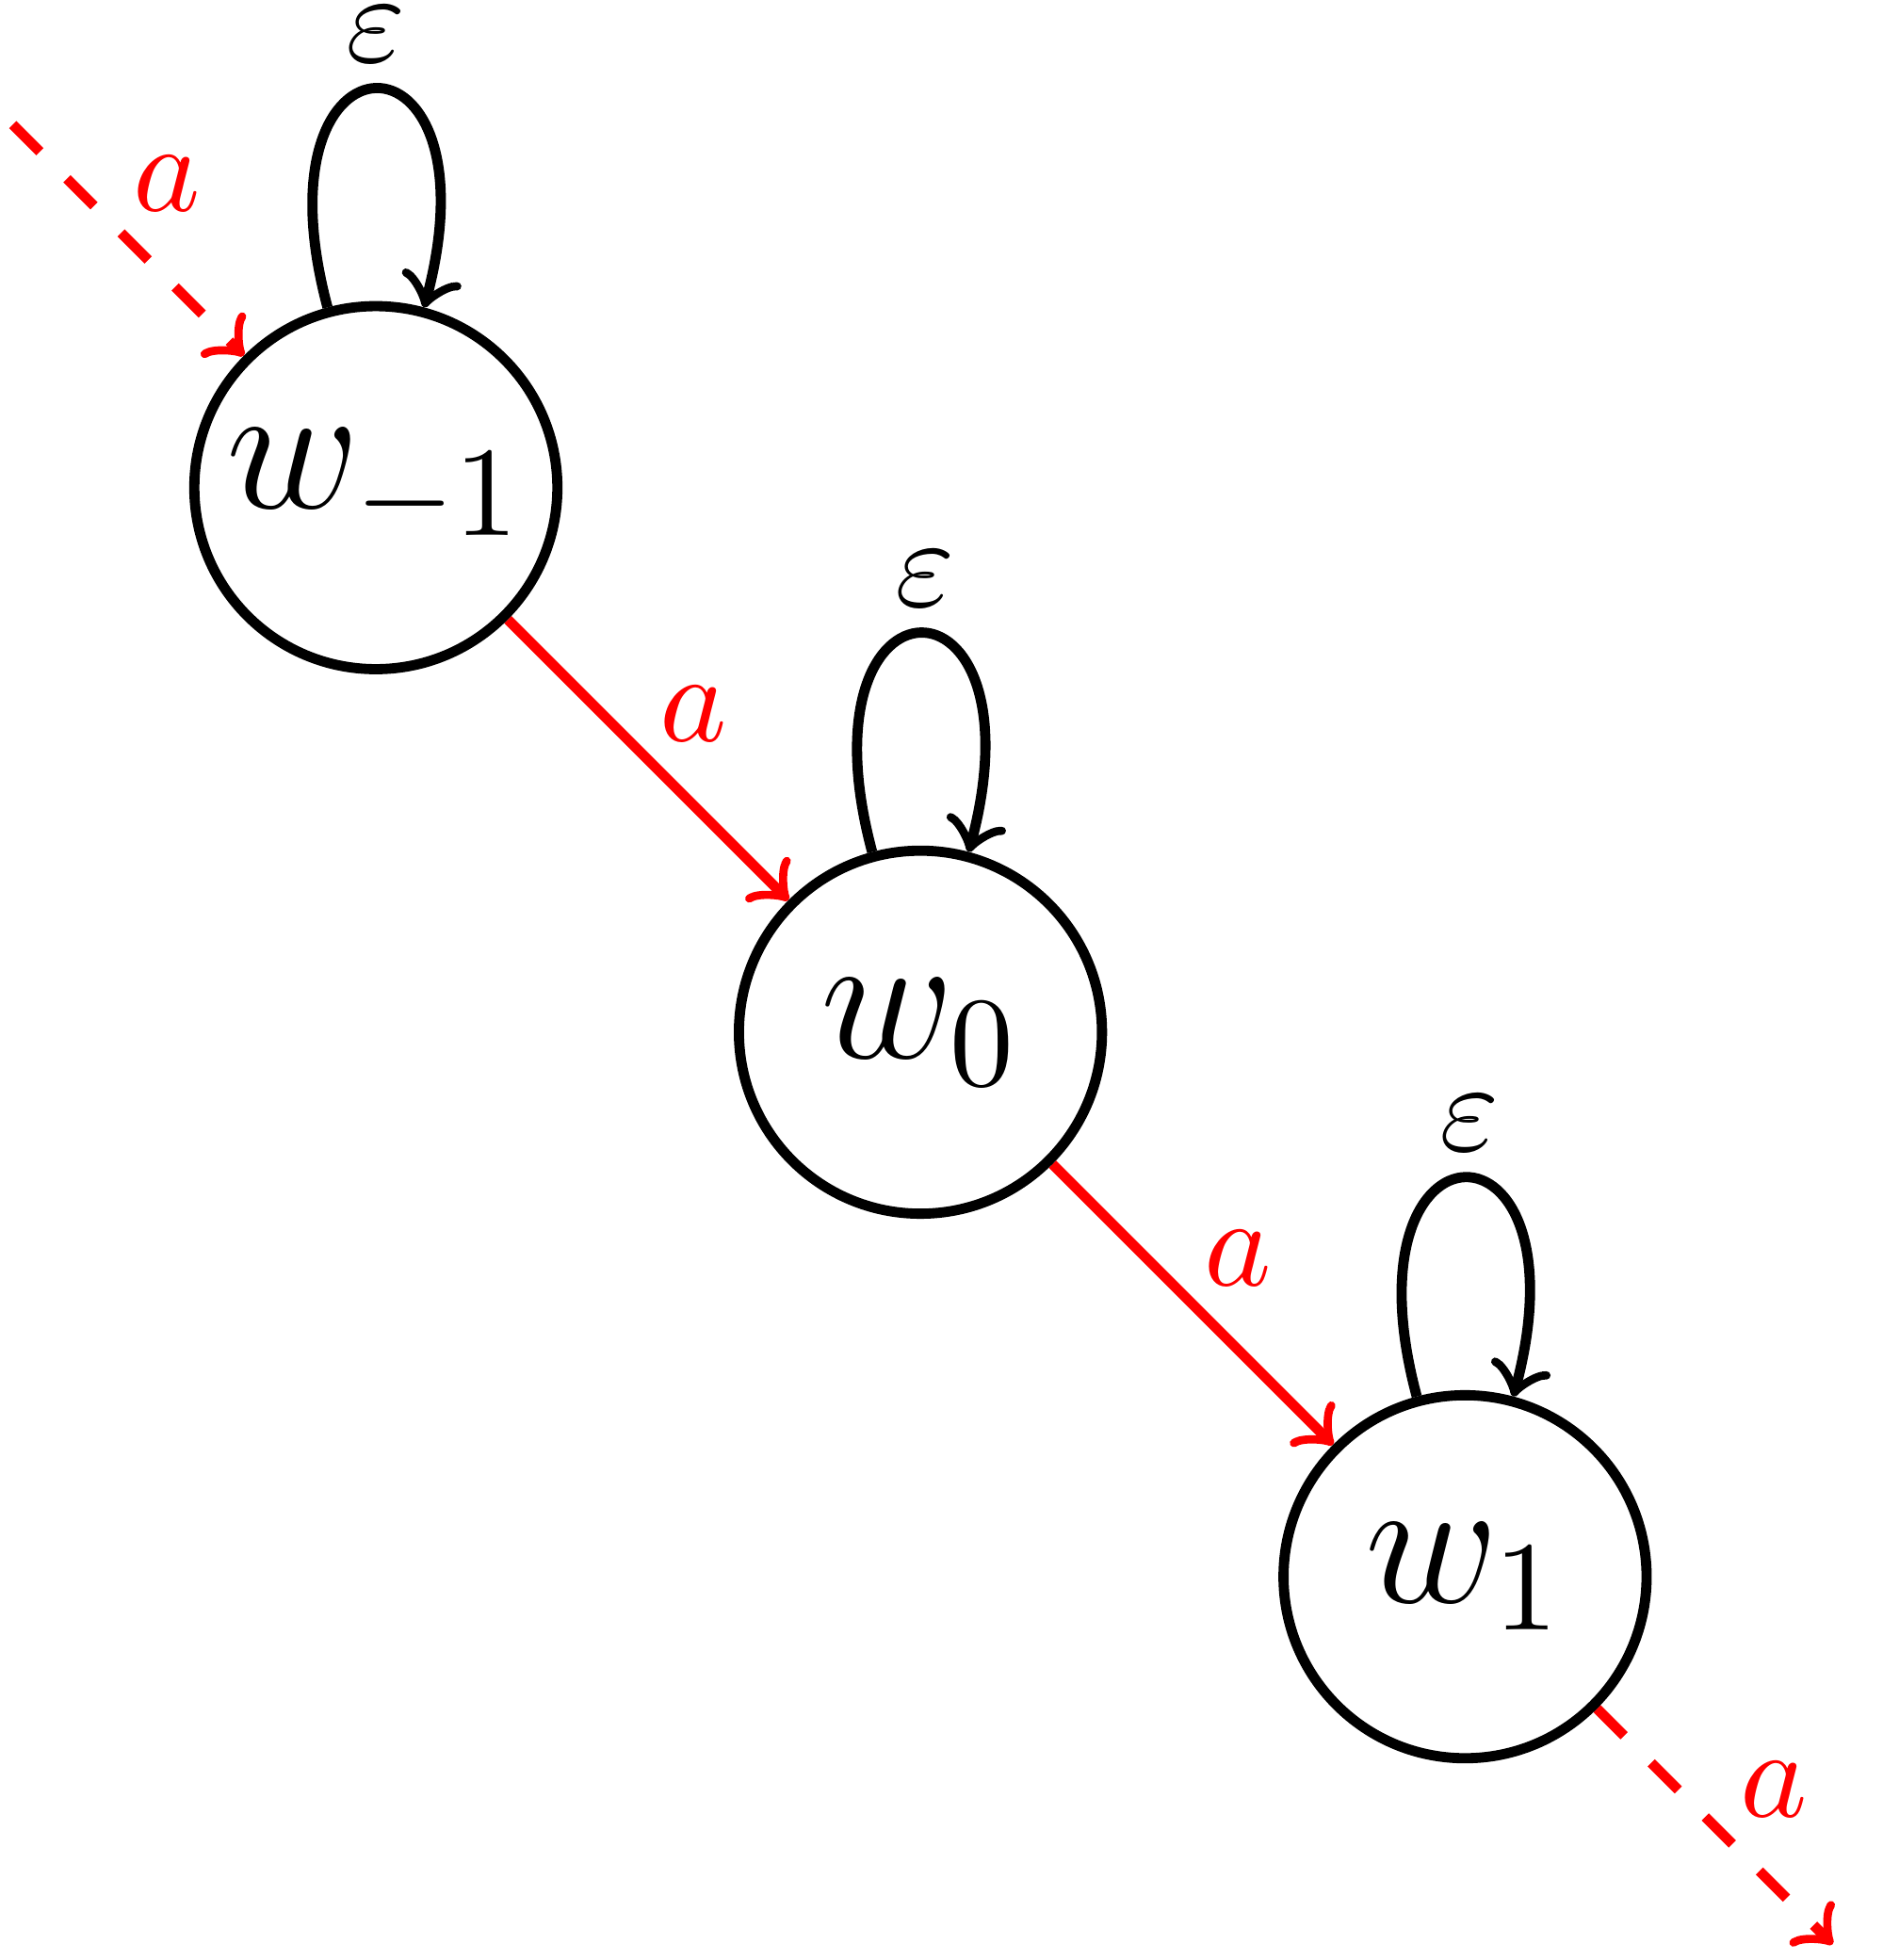
\includegraphics[width=0.5\linewidth]{6BeyondSBDRLLocalAlgebras/Images/infinite_double_linear_chain_world.png}
        \caption{
        \draftnote{blue}{To do}{Improve caption.}
        }
    \end{figure}}
    \begin{align}
        \epsilon \ast w_{i} = w_{i} \\
        a \ast w_{i} = w_{i+1}
    \end{align}

    \item \textbf{Irreversibility of $a$.}
    For $a$ to be reversible we need an $a' \in \hat{A}^{*}$ such that
    \begin{align}
        & a' \ast (a \ast w_{i}) = w_{i} \\
        \implies & a' \ast w_{i + 1} = w_{i}
    \end{align}
    In other words, we need $a'$ to decrease the index of the world state its applied to by 1.
    However, from $\hat{\ast}$ we can see that any sequence of $a$'s or $\epsilon$'s either do not change or increase the index of the world state they are applied to.
    Therefore, no such $a'$ exists in $\hat{A}^{*}$.

    \item \textbf{Vertex-transitivity.}
    For any $w_{i}, w_{j} \in W$, the automorphism
    \begin{equation}
    \begin{aligned}
        & \varphi_{(w_{i}, w_{j})}: W \to W \\
        & \varphi_{(w_{i}, w_{j})}(w_{k}) = w_{k+(j-i)}
    \end{aligned}
    \end{equation}
    maps $w_{i}$ to $w_{j}$ while preserving action labels.
\end{enumerate}
\end{proofE}


\begin{propositionE}[][normal]
    In vertex-transitive worlds, an action $a \in \hat{A}^{*}$ is irreversible from a world state $w \in W$ $\implies$ $a$ is globally irreversibility.
\end{propositionE}
\begin{proofE}
    \draftnote{blue}{To do}{
    Rework using action-homogeneous property proof.
    }
    \textbf{Proof by contradiction.}
    Suppose an action $a \in \hat{A}^{*}$ is irreversible from a world state $w \in W$.
    Therefore,
    \begin{equation}
        \text{an } a' \in \hat{A}^{*} \text{ does not exist such that } a' \ast (a \ast w) = w
    \end{equation}

    Assume that $a$ is reversible from some $w' \in W$.
    Therefore, there exists an $a' \in \hat{A}^{*}$ such that
    \begin{equation}
        a' \ast (a \ast w') = w'
    \end{equation}

    By vertex-transitivity, there exists an automorphism
    \begin{equation}
    \begin{aligned}
        & \varphi_{(w', w)}: W \to W \\
        & \varphi_{(w', w)}(w') = w
    \end{aligned}
    \end{equation}
    Therefore, we have
    \begin{align}
        & a' \ast (a \ast w') = w' \\
        \implies & (a' \circ a) \ast w' = w' \\
        \implies & \varphi_{(w', w)}((a' \circ a) \ast w') = \varphi_{(w', w)}(w') \\
        \implies & (a' \circ a) \ast \varphi_{(w', w)}(w') = \varphi_{(w', w)}(w') \\
        \implies & (a' \circ a) \ast w = w \\
        \implies & a' \ast (a \ast w) = w
    \end{align}
    Therefore, $a$ is reversible from $w$, which is a contradiction.
    This is a contradiction with the irreversibility of $a$ from $w$.
\end{proofE}



\begin{propositionE}\label{prp:vertex_transitive_finite_world_has_global_inverses}
     A world $\mathscr{W}$ is vertex-transitive and has finite $|W|$ $\implies$ every action in $\hat{A}^{*}$ has a global inverse.
\end{propositionE}
\begin{proofE}
\begin{enumerate}
    \item \textbf{Defining $f_{a}$.}
    Let $a \in \hat{A}^{*}$ an arbitrary action that is defined in at least one world state.
    Vertex-transitivity requires that the number of out-going $a$-labelled transformations is the same for every world, therefore each state must have at least one transformation $d : w \xrightarrow{a} a \ast w$.

    Due to the action uniqueness condition, there is exactly one $a$-labelled transformation leaving each world state.
    Therefore, the curried function
    \begin{equation}
    \begin{aligned}
        & f_{a}: W \to W \\
        & f_{a} := a \ast w
    \end{aligned}
    \end{equation}
    is well-defined and total on $W$

    \item \textbf{$f_{a}$ is injective.}
    We have seen that there is exactly one $a$-labelled transformation leaving each world state, therefore, there are $|W|$ $a$-labelled transformations leaving world states in total, and so there must be $|W|$ $a$-labelled transformations entering the $|W|$ world states in total.

    In vertex-transitive worlds, the number of in-going $a$-labelled transformations is the same for every world state and there are $|W|$ $a$-labelled transformations entering the $|W|$ world states.
    Therefore, each world state must have exactly one in-going $a$-labelled transformation.

    If $f_{a}(w_{1}) = f_{a}(w_{2}) = w'$ for two distinct world states $w_{1}, w_{2} \in W$, then $w'$ would have two in-going $a$-labelled transformations, which is a contradiction since each world state must have exactly one in-going $a$-labelled transformation.
    Therefore $f_{a}$ must be injective.

    \item \textbf{$f_{a}$ is surjective.}
    For a finite set $W$, an injective function $f_{a}: W \to W$ must map all $|W|$ elements to $|W|$ distinct elements in $W$.
    Therefore $f_{a}$ maps $W$ into itself, and so $f_{a}$ is surjective.

    \item \textbf{$f_{a}$ is a permutation.}
    Since $f_{a}$ is injective and surjective, $f_{a}$ is bijective.
    A bijection from a finite set $W$ to itself is a permutation.
    Therefore, $f_{a}$ decomposes $W$ into disjoint cycles:
    \begin{equation}
        W = C_{1} \sqcup ... \sqcup C_{k} \quad \text{where } C_{i} = \{a^{j} \ast w \mid j \in \mathbb{N}\}
    \end{equation}

    \item \textbf{Vertex-transitivity $\implies$ all cycles have the same length.}
    Consider a world state $w_{i} \in C_{i}$ and a world state $w_{j} \in C_{j}$.
    By vertex-transitivity, there exists an automorphism $\varphi_{(w_{i}, w_{j})}(w_{i}) = w_{j}$.
    Since $\varphi_{(w_{i}, w_{j})}$ preserves labelled transformations, $\varphi_{(w_{i}, w_{j})}$ maps $C_{i}$ to a new cycle $\varphi_{(w_{i}, w_{j})}(C_{i})$ which must be of length $|C_{i}|$.
    But $\varphi_{(w_{i}, w_{j})}(w_{i}) = w_{j}$ therefore $\varphi_{(w_{i}, w_{j})}(C_{i})$ must include $w_{j}$ and so the structures of $\varphi_{(w_{i}, w_{j})}(C_{i})$ and $C_{j}$ must align.
    Therefore, $\varphi_{(w_{i}, w_{j})}(C_{i}) = C_{j}$ and so $|C_{i}| = |C_{j}|$ because automorphisms preserve the number of transforms in cycles.

    Therefore, $f_{a}$ decomposes $W$ into disjoint cycles of length $n$:
    \begin{equation}\label{eqn:fa_decomposes_W_into_disjoint_cycles}
    \begin{aligned}
        W = & C_{1} \sqcup ... \sqcup C_{k} \\
        & \text{where } C_{i} = \{a^{j} \ast w \mid j \in \mathbb{N}\} \text{ and } |C_{i}| = n
    \end{aligned}
    \end{equation}

    \item \textbf{Presence of global inverse.}
    From \cref{eqn:fa_decomposes_W_into_disjoint_cycles}, we have
    \begin{align}
        & a^{n} \ast w = w \\
        \implies & a^{n-1} \ast (a \ast w) = w
    \end{align}
    Similarly, we have
    \begin{align}
        & a^{n} \ast w = w \\
        \implies & a \ast (a^{n-1} \ast w) = w
    \end{align}
    Therefore, $a^{n-1}$ is a global inverse of $a$

    \item \textbf{Conclusion.}
    Since the choice of $a$ is arbitrary, every action in $\hat{A}^{*}$ has a global inverse.
\end{enumerate}
\end{proofE}


\begin{corollary}
    A world $\mathscr{W}$ is vertex-transitive and has finite $|W|$ $\implies$ all actions in $\hat{A}^{*}$ are reversible (i.e., $\mathscr{W}$ is a reversible world \draftnote{blue}{To do}{Check we have defined "reversible world"}).
\end{corollary}

\begin{corollary}
    A world $\mathscr{W}$ is vertex-transitive and has finite $|W|$ $\implies$ $\mathscr{W}$ has no irreversible actions.
\end{corollary}

\begin{corollary}
    The only vertex-transitive worlds that can contain irreversible actions are those where $|W|$ is infinite.
\end{corollary}


\begin{propositionE}[][normal]
    A world $\mathscr{W}$ is vertex-transitive and has finite $|W|$ $\implies$ $(\hat{A}^{*}/\sim, \circ_{\sim})$ is a group.
    
\end{propositionE}
\begin{proofE}
\begin{enumerate}
    \item \textbf{Total.}
    \draftnote{blue}{To do}{}

    \item \textbf{Associativity and identity.}
    Follow from \cref{prp:A_sim_is_monoid}.

    \item \textbf{Inverses.}
    Follows from \cref{prp:vertex_transitive_finite_world_has_global_inverses} and \cref{prp:global_inverse_means_inverse_in_global_algebra}.
\end{enumerate}
\end{proofE}


\begin{propositionE}[][normal]
    \draftnote{blue}{To do}{}
    In vertex-transitive worlds,
    \begin{enumerate}
        \item $a'$ is left inverse of a world state $w \in W$ $\implies$ $a'$ is a global left inverse of $a$.
        \item $a'$ is right inverse of a world state $w \in W$ $\implies$ $a'$ is a global right inverse of $a$.
        \item $a'$ is inverse of a world state $w \in W$ $\implies$ $a'$ is a global inverse of $a$.
    \end{enumerate}
\end{propositionE}
\begin{proofE}
    \draftnote{blue}{To do}{
    Use action-homogeneous property proof.
    }
\end{proofE}

\begin{propositionE}
    A world $\mathscr{W}$ is vertex-transitive $\implies$ $\mathscr{W}^{\hat{A}\to}(w) \cong \mathscr{W}^{\hat{A}\to}(w')$ for all $w, w' \in \mathscr{W}^{\hat{A}\to}(w)$ (i.e., all reachable world states are isomorphic).
    \draftnote{blue}{Consider}{
    Is this true for $w,w' \in W$ ?
    }
\end{propositionE}
\begin{proofE}
\draftnote{blue}{Consider}{
Do we need to include something about $D_{A}$ vs $\hat{D}_{A}$ and $D_{A}^{\hat{A}\to}(w)$ (which hasn't been defined ?) vs $\hat{D}_{A}^{\hat{A}\to}(w)$.
}
\begin{enumerate}
    \item \textbf{Existence of automorphisms.}
    By vertex-transitivity, we have an automorphism
    \begin{equation}
    \begin{aligned}
        & \varphi_{(w,w')}: W \to W \\
        & \varphi_{(w,w')}(w) = w'
    \end{aligned}
    \end{equation}
    and an induced bijection
    \begin{equation}
        \Phi_{(w,w')}: D_{A} \to D_{A}
    \end{equation}
    such that for every $d \in D_{A}$ with $d: u \xrightarrow{a} v$ we have
    \begin{align}
        & \Phi_{(w,w')}(d): \varphi_{(w,w')}(u) \xrightarrow{a} \varphi_{(w,w')}(v), \quad \text{and} \\
        & l(\Phi_{(w,w')}(d)) = l(d)
    \end{align}

    \item \textbf{Restriction to reachable subworlds.}
    We now define the restriction maps:
    \begin{align}
        & \varphi^{\text{reach}}_{(w,w')} := \varphi_{(w,w')}|_{W^{\hat{A}\to}(w)}, \quad \text{and} \\
        & \Phi^{\text{reach}}_{(w,w')} := \Phi_{(w,w')}|_{\hat{D}_{A}^{\hat{A}\to}(w)}
    \end{align}
    We will show that $\varphi^{\text{reach}}_{(w,w')}$ and $\Phi^{\text{reach}}_{(w,w')}$ establish an isomorphism between $\mathscr{W}^{\hat{A}\to}(w)$ and $\mathscr{W}^{\hat{A}\to}(w')$.

    \item \textbf{Mapping of world states.}
    Consider an arbitrary $u \in W^{\hat{A}\to}(w)$.
    By definition of $W^{\hat{A}\to}(w)$, there exists a transformation $d \in D_{A}$ such that $d: w \xrightarrow{a} u$ where $a \in \hat{A}^{*}$.
    
    Applying $\varphi_{(w,w')}^{\text{reach}}$ to $d$ gives
    \begin{align}
        & d: w \xrightarrow{a} u \\
        \implies & \Phi_{(w,w')}^{\text{reach}}(d): \varphi_{(w,w')}^{\text{reach}}(w) \xrightarrow{a} \varphi_{(w,w')}^{\text{reach}}(u) \\
        \implies & \Phi_{(w,w')}^{\text{reach}}(d): w' \xrightarrow{a} \varphi_{(w,w')}^{\text{reach}}(u) \\
        \implies & \varphi_{(w,w')}^{\text{reach}}(u) \in W^{\hat{A}\to}(w')
    \end{align}
    Therefore, we have
    \begin{equation}
        \varphi_{(w,w')}^{\text{reach}}(W^{\hat{A}\to}(w)) \subseteq W^{\hat{A}\to}(w')
    \end{equation}

    Since $\varphi_{(w,w')}^{\text{reach}}$ is bijective with inverse $\varphi_{(w',w)}^{\text{reach}}$, it follows that
    \begin{equation}
        \varphi_{(w',w)}^{\text{reach}}(W^{\hat{A}\to}(w')) \subseteq W^{\hat{A}\to}(w)
    \end{equation}

    Therefore, we have
    \begin{equation}
        \varphi_{(w,w')}^{\text{reach}}(W^{\hat{A}\to}(w)) = W^{\hat{A}\to}(w')
    \end{equation}

    \item \textbf{Mapping of transformations.}
    $\Phi_{(w,w')}^{\text{reach}}$ is bijective because $\Phi_{(w,w')}$ is bijective and $\varphi_{(w',w)}^{\text{reach}}$ maps state isomorphically. 
    $\Phi_{(w,w')}^{\text{reach}}$ also preserves labels ($l(\Phi_{(w,w')}^{\text{reach}}(d)) = l(d)$.
    
    \item \textbf{Conclusion.}
    Since $(\varphi_{(w,w')}^{\text{reach}}, \Phi_{(w,w')}^{\text{reach}})$ consists of bijections between the corresponding state sets that preserves sources, target and labels of transformations, it follows that $\mathscr{W}^{\hat{A}\to}(w)$ and $\mathscr{W}^{\hat{A}\to}(w')$ are isomorphic.
\end{enumerate}
\end{proofE}


%%%%%%%%%%%%%%%%%%%%%%%%%%%%%%%%%%%
\paragraph{
\draftnote{blue}{Insert section title}{}
}

\begin{propositionE}
     $T_{\sim_{w}}(\hat{A}^{*}, \circ) = T_{\sim_{w'}}(\hat{A}^{*}, \circ)$ for all $w, w' \in W$ $\centernot\implies$ vertex-transitive world.
\end{propositionE}
\begin{proofE}
\textbf{Proof by example.}
\begin{enumerate}
    \item \textbf{Defining a binary tree world $\mathscr{W}$.}
    Consider a world-agent pair with $W = \{w_{i}\}$ where $i \in \{0, 1\}^{*}$\footnote{
    $\{0, 1\}^{*}$ is the set of all finite words over $\{0, 1\}$ produced by the Kleene star operator:
    \begin{equation}
        W = \{ w_{\epsilon}, w_{0}, w_{1}, w_{00}, w_{01}, w_{10}, w_{11}, \dots \}
    \end{equation}
    }, and $\hat{\ast}$ given by\footnote{
    \begin{figure}[H]
        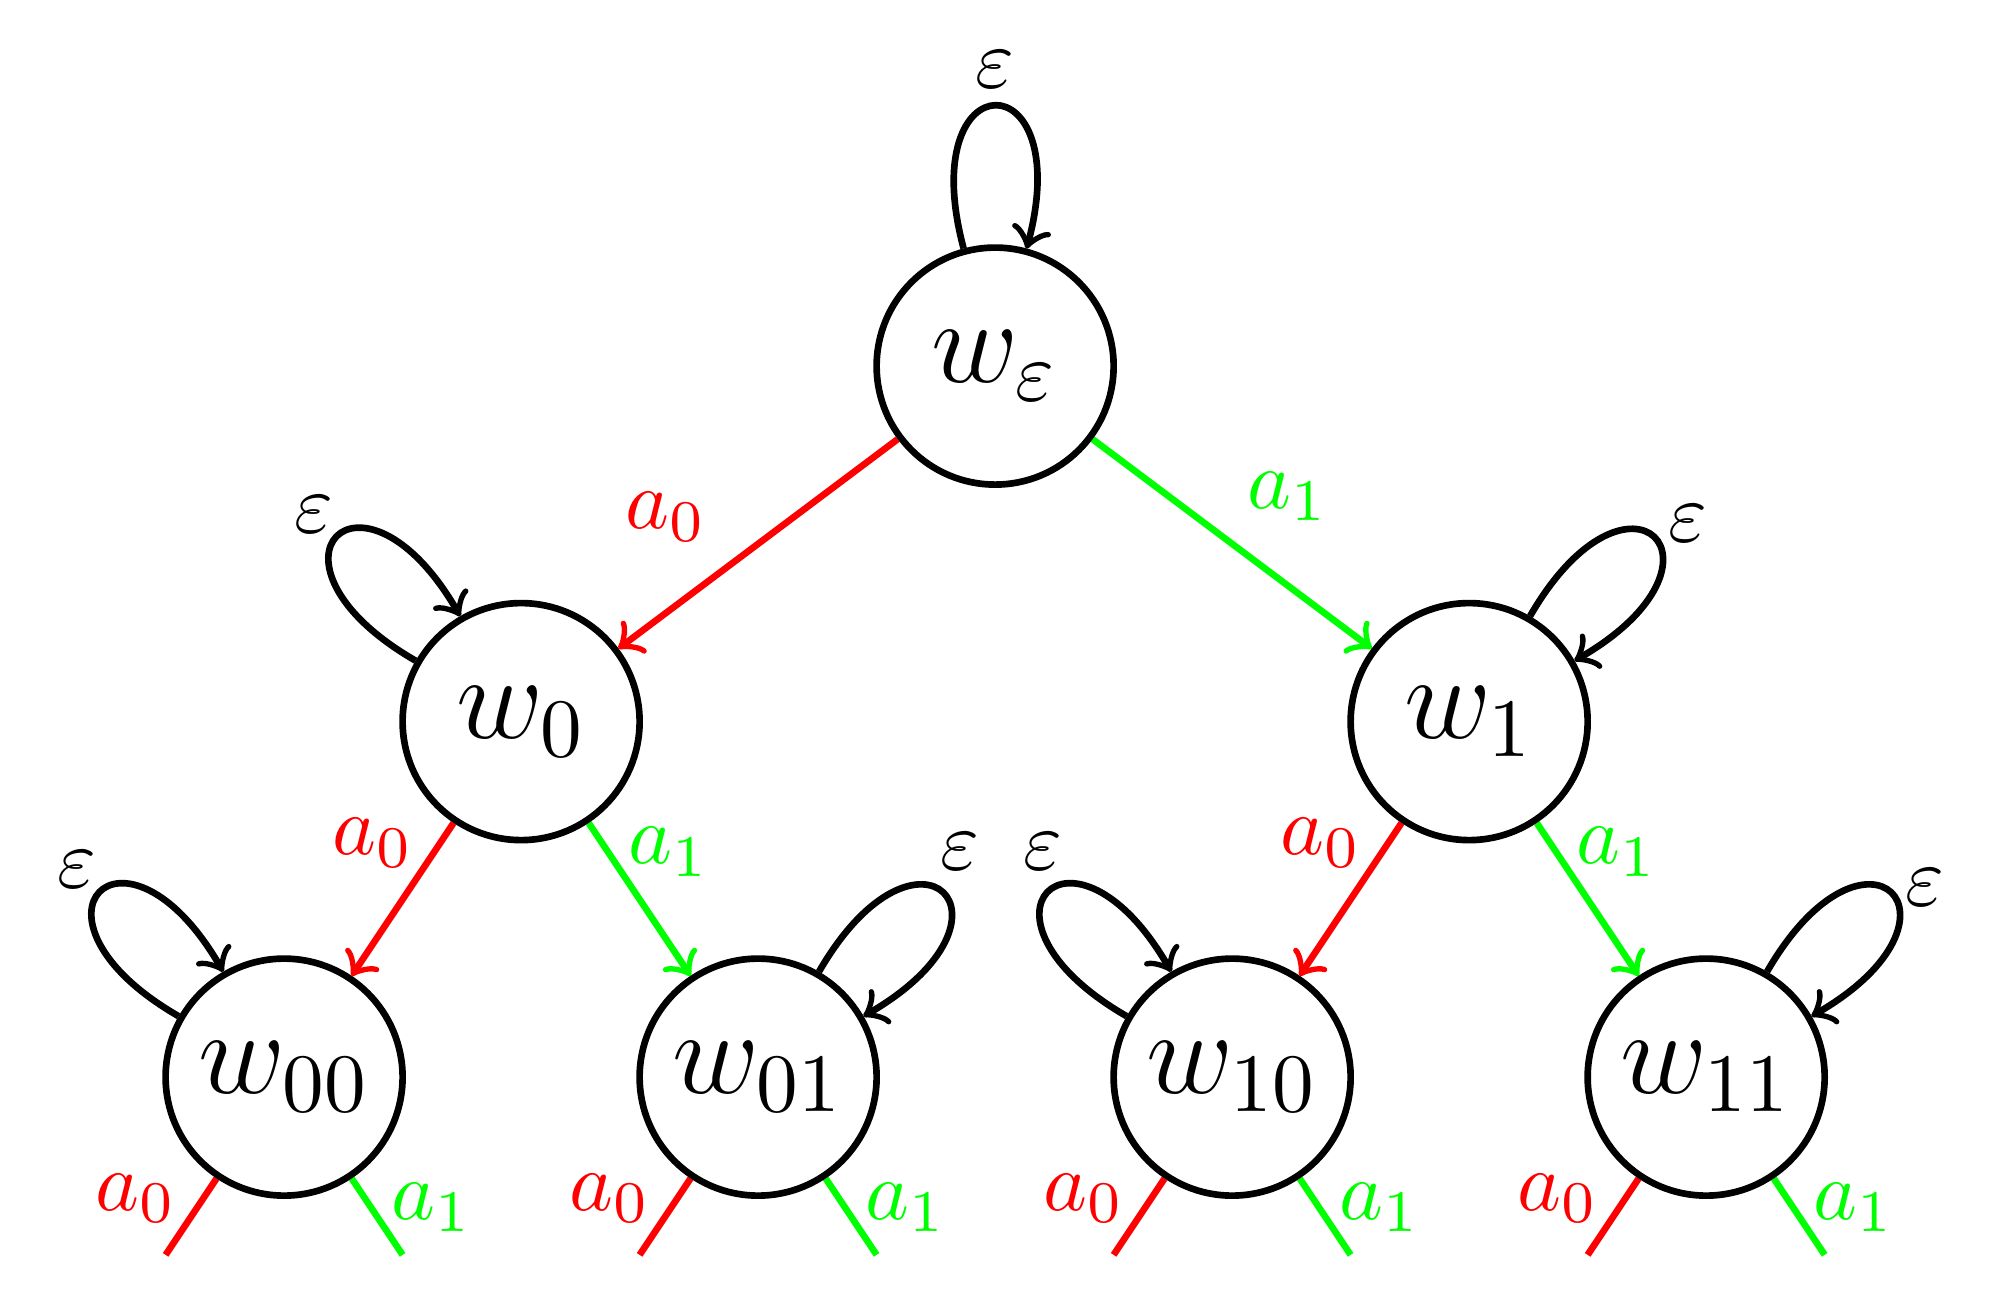
\includegraphics[width=0.5\linewidth]{6BeyondSBDRLLocalAlgebras/Images/binary_tree_world.png}
        \caption{\draftnote{blue}{To do}{Caption.}}
    \end{figure}
    }
    \begin{align}
        & \epsilon \ast w_{i} = w_{i} \\
        & \hat{a}_{0} \ast w_{i} = w_{i0} \\
        & \hat{a}_{1} \ast w_{i} = w_{i1}
    \end{align}

    \item \textbf{$\mathscr{W}$ is not vertex-transitive.}
    The root world state $w_{\epsilon}$ has zero in-going transformations, while all other world states have one in-going transformation.
    Therefore, from \cref{prp:vertex_transitive_implies_num_ingoing_equals_num_outgoing}, $\mathscr{W}$ is not vertex-transitive.

    \item \textbf{Local Cayley tables are identical.}
    \begin{enumerate}
        \item \textbf{Defining a map.}
        We define the map
        \begin{align}
            & \phi_{w}: \hat{A}^{*} \to W \\
            & \phi_{w}(a) := a \ast w
        \end{align}

        \item \textbf{$\phi_{w}$ is injective.}
        Consider an arbitrary world state $w_{i}$ and two actions $a_{j}, a_{k} \in \hat{A}^{*}$ where $i,j,k \in \{0,1\}^{*}$ and $a_{j} \sim_{w_{i}} a_{k}$.

        From the definition of $\sim_{w}$ we have
        \begin{align}
            & a_{j} \sim_{w_{i}} a_{k} \\
            \implies & a_{j} \ast w_{i} = a_{k} \ast w_{i} \\
            \implies & w_{ij} = w_{ik}
        \end{align}
        Since each world state is uniquely indexed by the sequence of minimum actions it takes to get to that world state from the root world state $w_{\epsilon}$, we have
        \begin{align}
            & w_{ij} = w_{ik} \\
            \implies & j = k \\
            \implies & a_{j} = a_{k}
        \end{align}
        Therefore, $\phi_{w}$ is injective.

        \item \textbf{Local equivalence classes are singletons.}
        From injectivity of $\phi_{w}$, we have
        \begin{align}
            & a \sim_{w} a' \\
            \implies & a \ast w = a' \ast w \\
            \implies & \phi_{w}(a) = \phi_{w}(a') \\
            \implies & a = a'
        \end{align}
        Therefore, each local equivalence class $[a]_{\sim_{w}} \subseteq \hat{A}^{*}$ is a singleton:
        \begin{align}
            & [a]_{\sim_{w}} = \{a\} \quad \text{for every $a \in \hat{A}^{*}$} \\
            \implies & \hat{A}^{*}/\sim_{w} \cong \hat{A}^{*}
        \end{align}

        \item \textbf{Local Cayley tables are identical.}
        $\sim_{w}$ is the identity on $\hat{A}^{*}$ where the elements of $\hat{A}^{*}/\sim_{w}$ are the singletons $\{a\}$ and $\circ_{\sim_{w}}$ is the concatenation of words.
        Therefore, $T_{\sim_{w}}(\hat{A}^{*}, \circ)$ is the Cayley table of the free monoid on the generators $\{\hat{a}_{0}, \hat{a}_{1}\}$ for all $w \in W$.
    \end{enumerate}
\end{enumerate}
\end{proofE}

\begin{propositionE}[][normal]
     $\mathscr{W}$ where $|W|$ is finite and $T_{\sim_{w}}(\hat{A}^{*}, \circ) = T_{\sim_{w'}}(\hat{A}^{*}, \circ)$ for all $w, w' \in W$ $\implies$ $\mathscr{W}$ is vertex-transitive.
\end{propositionE}
\begin{proofE}
    \draftnote{red}{To do}{Prove for action-homogeneous.}
\begin{enumerate}
    \item 
\end{enumerate}
\end{proofE}


\draftnote{red}{OTHER}{}



\draftnote{blue}{ (as footnote somewhere?)}{
There are no state specific actions - this resembles a homogeneous space in algebraic topology.
}

\draftnote{blue}{To do in one of the previous sections}{
Does the Cayley table counting formula mean that, for a given world, each there are the same number of local Cayley table constructions for each $w \in W$ ?
}

\begin{propositionE}
    Vertex-transitive world $\implies$ $\circ_{\sim_{w}}$ is well-defined for all $w \in W$.
\end{propositionE}
\begin{proofE}
    \draftnote{blue}{To do}{
    Rework using action-homogeneous $\circ_{\sim_{w}}$ is well-defined proof.
    }
\begin{enumerate}
    \item \textbf{Aim.}
    We need to show that for a vertex-transitive world,
    \begin{equation}
        a \sim_{w} a' \text{ and } b \sim_{w} b' \implies (a \circ b) \sim_{w} (a' \circ b')
    \end{equation}

    \item \textbf{Set up.}
    Let $a, a', b, b' \in \hat{A}^{*}$ such that $a \sim_{w} a'$ and $b \sim_{w} b'$.
    By the definition of $\sim_{w}$, we have
    \begin{align}
        & a \sim_{w} a' \implies a \ast w = a' \ast w = w_{1} \\
        & b \sim_{w} b' \implies b \ast w = b' \ast w = w_{2}
    \end{align}

    \item \textbf{Simplifying our aim.}
    \begin{align}
        & (a \circ b) \ast w = a \ast (b \ast w) = a \ast w_{2} \\
        & (a' \circ b') \ast w = a' \ast (b' \ast w) = a' \ast w_{2}
    \end{align}

    \item \textbf{Using vertex-transitivity.}
    $\mathscr{W}$ is vertex-transitive, therefore these exists an automorphism $\varphi_{(w, w_{2})}: W \to W$ such that $\varphi_{(w, w_{2})}(w) = w_{2}$.
    For $a \ast w = w_{1}$,
    \begin{align}
        & a \ast w = w_{1} \\
        \implies & \varphi_{(w, w_{2})}(a \ast w) = \varphi_{(w, w_{2})}(w_{1}) \\
        \implies & a \ast \varphi_{(w, w_{2})}(w) = \varphi_{(w, w_{2})}(w_{1}) \\
        \implies & a \ast w_{2} = \varphi_{(w, w_{2})}(w_{1})
    \end{align}
    Similarly for $a' \ast w = w_{1}$,
    \begin{align}
        & a' \ast w = w_{1} \\
        \implies & \varphi_{(w, w_{2})}(a' \ast w) = \varphi_{(w, w_{2})}(w_{1}) \\
        \implies & a' \ast \varphi_{(w, w_{2})}(w) = \varphi_{(w, w_{2})}(w_{1}) \\
        \implies & a' \ast w_{2} = \varphi_{(w, w_{2})}(w_{1})
    \end{align}
    Therefore, we have
    \begin{align}
        & a \ast w_{2} = a' \ast w_{2} \\
        \implies & (a \circ b) \ast w = (a' \circ b') \ast w \\
        \implies & (a \circ b) \sim_{w} (a' \circ b')
    \end{align}
\end{enumerate}
\end{proofE}

%%%%%%%%%%%%%%%%%%%%%%%%%%%%%%%%%%%%%%%%%
\subsection{Action-homogeneous worlds}
\draftnote{green}{To do}{
\begin{enumerate}
    \item \textbf{Homogenous actions proofs}
    \begin{enumerate}
        \item \textbf{Proof.}
        Global consistent inverse means both actions are homogeneous ?
        \item \textbf{Corollary:} $\circ_{\sim_{w}}$ well-defined for composition of homogeneous actions even in action inhomogeneous worlds (check).
        \item \textbf{Proof.}
        Subset of homogeneous actions forms a group ?
    \end{enumerate}
\end{enumerate}
}

\draftnote{blue}{Include}{
Intro paragraph about "Considering the agent's perspective".
From the perspective of an agent in a Markov process, the infinite binary tree world containing a root world state $w_{0}$ with no incoming transformations is the same as a world with an infinite binary tree with no root since the agent can only interact with reachable world states.
Can we come up with a property of worlds that is not as restrictive as the vertex-transitive condition but gives us the same uniform algebraic structure that we find in vertex-transitive worlds and also in the infinite binary tree worlds with a root world state ?
}

\draftnote{blue}{To do}{
Check in proofs that $\mathscr{W}^{\hat{A}\to}(w')$ and $W^{\hat{A}\to}(w)$ are used in the correct places.
}

\begin{definition}[Action-homogeneous world]\label{def:action_homogeneous}
    A world $\mathscr{W}$ is called \emph{action-homogeneous} from a world state $w \in W$ if there exists a label-preserving directed multigraph isomorphism
    \begin{equation}
        \phi_{(w,w')}: \mathscr{W}^{\hat{A}\to}(w) \to \mathscr{W}^{\hat{A}\to}(w')
    \end{equation}
    for all $w' \in W^{\hat{A}\to}(w)$.
\end{definition}

\draftnote{blue}{To do}{
Check this is how the isomorphism is defined in proofs to make them consistent.
}

\paragraph{Properties of $\phi_{(w,w')}$.}
The isomorphism in \cref{def:action_homogeneous} is made up of a bijection
\begin{equation}
    \phi_{(w,w'), W}: W^{\hat{A}\to}(w) \to W^{\hat{A}\to}(w')
\end{equation}
between world states, and a bijection
\begin{equation}
    \phi_{(w,w'), D}: \hat{D}_{A}^{\hat{A}\to}(w) \to \hat{D}_{A}^{\hat{A}\to}(w')
\end{equation}
between minimum action transformations\footnote{\draftnote{blue}{To do}{Footnote about why mapping the minimum action transformations means the bijection works for all labelled transformations.}}.
$\phi_{W,(w,w')}$ and $\phi_{D,(w,w')}$ satisfy the following:
\begin{enumerate}
    \item \textbf{Preservation of identities.}
    For any world state $x \in W^{\hat{A}\to}(w)$,
    \begin{equation}
        \phi_{(w,w'), D}(1_{x}) = 1_{\phi_{W,(w,w')}(x)}
    \end{equation}

    \item \textbf{Preservation of composition.}
    For any transformations $d_{1}, d_{2} \in D_{A}^{\hat{A}\to}(w)$,
    \begin{equation}
        \phi_{(w,w'), D}(d_{2} \circ d_{1}) = \phi_{(w,w'), D}(d_{2}) \circ \phi_{(w,w'), D}(d_{1})
    \end{equation}

    \item \textbf{Preservation of source and target maps.}
    For any transformation $d \in D_{A}^{\hat{A}\to}(w)$,
    \begin{equation}
        s(\phi_{(w,w'), D}(d)) = \phi_{(w,w'), W}(s(d))
    \end{equation}
    and
    \begin{equation}
        t(\phi_{(w,w'), D}(d)) = \phi_{(w,w'), W}(t(d))
    \end{equation}

    \item \textbf{Preservation of transformation labels.}
    For any transformation $d \in D_{A}^{\hat{A}\to}(w)$,
    \begin{equation}
        l(d) = l(\phi_{(w,w'), D}(d))
    \end{equation}
\end{enumerate}

We can convert the effect of the transformation isomorphism $\phi_{(w,w'), D}$ into an action-equivariance condition on the world state isomorphism $\phi_{(w,w'), W}$.
For any world state $x \in W^{\hat{A}\to}(w)$ and for any action $a \in \hat{A}^{*}$,\footnote{
    This action-equivariance condition comes from the fact that the order of applying the isomorphism to the world state $x$ then applying $a \ast$ should be the same as applying $a \ast$ then applying the isomorphism.
% https://q.uiver.app/#q=WzAsNCxbMCwwLCJ4Il0sWzAsMiwiXFxwaGlfe1d9KHgpIl0sWzIsMCwiYSBcXGFzdCB4Il0sWzIsMiwiXFxwaGlfe1d9KGEgXFxhc3QgeCkgPSBhIFxcYXN0IFxccGhpX3tXfSh4KSJdLFswLDIsImEgXFxhc3QiXSxbMSwzLCJhIFxcYXN0Il0sWzIsMywiXFxwaGlfe1d9Il0sWzAsMSwiXFxwaGlfe1d9Il1d
\[\begin{tikzcd}[ampersand replacement=\&]
	x \&\& {a \ast x} \\
	\\
	{\phi_{W}(x)} \&\& {\phi_{W}(a \ast x) = a \ast \phi_{W}(x)}
	\arrow["{a \ast}", from=1-1, to=1-3]
	\arrow["{\phi_{W}}", from=1-1, to=3-1]
	\arrow["{\phi_{W}}", from=1-3, to=3-3]
	\arrow["{a \ast}", from=3-1, to=3-3]
\end{tikzcd}\]
    }
\begin{equation}
    \phi_{(w,w'), W}(a \ast x) = a \ast \phi_{(w,w'), W}(x)
\end{equation}
whenever $a \ast x$ is defined.

The equivariance condition on $\phi_{(w,w'), W}$ guarantees that the labelled directed multigraph structure of $\mathscr{W}^{\hat{A}\to}(w)$ is preserved.
Therefore, if we construct an isomorphism with
\begin{equation}
    \phi_{(w,w')}: \mathscr{W}^{\hat{A}\to}(w) \to \mathscr{W}^{\hat{A}\to}(w')
\end{equation}
that satisfies, for all $x \in \mathscr{W}^{\hat{A}\to}(w)$ and for all $a \in \hat{A}^{*}$ where $a \ast x$ is defined,
\begin{align}
    & \phi_{W,(w,w')}(w) = w' \\
    & \phi_{W,(w,w')}(a \ast x) = a \ast \phi_{W,(w,w')}(x),
\end{align}
then we have an isomorphism that preserves the labelled directed multigraph structure of $\mathscr{W}^{\hat{A}\to}(w)$ \footnote{
Because every transformation is uniquely identified by its source world state and its label, the transformation map $\phi_{D,(w,w')}$ is determined by the world state map $\phi_{D,(w,w')}$.
In other words, if we defined an isomorphism $\phi_{W,(w,w')}(w) = w'$ that is equivariant then, for each transformation $x \xrightarrow{a} a \ast x$, the isomorphism preserves the unique corresponding transformation $\phi_{W,(w,w')}(x) \xrightarrow{a} a \ast \phi_{W,(w,w')}(x)$.
}
.
For that reason, we can write $\phi_{(w,w')}$ when we mean $\phi_{W,(w,w')}$.

%%%%%%%%%%%%%%%%%%%%%%%%%%%%%%%%%%%%%%%%%%
\paragraph{Constructing $\phi_{(w,w')}$.}

A natural way to construct the isomorphism $\phi_{(w,w')}$ for $w \in W$ and $w' \in W^{\hat{A}\to}(w)$ is to transport the structure of $\mathscr{W}^{\hat{A}\to}(w)$ to $\mathscr{W}^{\hat{A}\to}(w')$ using a \emph{transporter action} $a \in \hat{A}^{*}$ that sends $w$ to $w'$.

By the definition of $W^{\hat{A}\to}(w)$, there exists an action $a \in \hat{A}^{*}$ with\footnote{
It is possible to have multiple actions that send $w$ to $w'$, but we only need one.
If the world is action-homogeneous from $w$, then these actions will be equivalent under $(\sim)_{w}$ and $\sim_{w}$.
}
\begin{equation}
    a \ast w = w'.
\end{equation}
We then define the world state part of the isomorphism by
\begin{equation}
    \phi(x) := a \ast x \quad \text{for all $x \in W^{\hat{A}\to}(w)$}
\end{equation}
Note that this sends the base state $w$ to
\begin{equation}
    \phi(w) = a \ast w = w'
\end{equation}


\draftnote{red}{UP NEXT}{
\begin{enumerate}
    \item Constructing $\phi_{(w,w')}$ using an "action-transporter".
    \item Inverse of $\phi_{(w,w')}$ still exists without an action.
    \item Existence of the isomorphism between any two reachable subworlds in $\mathscr{W}^{\hat{A}\to}(w)$.
    \item Check proofs.
\end{enumerate}
}
------

The isomorphism in \cref{def:action_homogeneous} is defined as follows:
If $\mathscr{W}$ is action-homogeneous from $w$, then for any two world states $w', w'' \in W^{\hat{A}\to}(w)$ there exists a directed multigraph isomorphism\footnote{
You'll notice that these isomorphisms are between any two world states $w', w'' \in \mathscr{W}^{\hat{A}\to}(w)$, rather than just between $w$ and a world state $w' \in \mathscr{W}^{\hat{A}\to}(w)$.
This is because
\begin{align}
        & \mathscr{W}^{\hat{A}\to}(w) \cong \mathscr{W}^{\hat{A}\to}(w') \\
        \text{ and } &  \mathscr{W}^{\hat{A}\to}(w) \cong \mathscr{W}^{\hat{A}\to}(w'') \\
    \implies & \mathscr{W}^{\hat{A}\to}(w') \cong \mathscr{W}^{\hat{A}\to}(w'').
\end{align}
}
\begin{align}
    & \phi_{(w', w'')}: \mathscr{W}^{\hat{A}\to}(w') \to \mathscr{W}^{\hat{A}\to}(w'') \\
    & \phi_{(w', w'')}(w') = w''
\end{align}
of subworlds such that for any $u \in W^{\hat{A}\to}(w')$ and any action $b \in \hat{A}^{*}$ for which $b \ast u$ is defined, we have
\draftnote{blue}{To do}{Put commuting diagram as footnote.}
\begin{equation}
    \phi_{(w', w'')}(b \ast u) = b \ast \phi_{(w', w'')}(u)
\end{equation}
\draftnote{blue}{Consider}{
Does the equivariance in the isomorphism here mean there is some sort of natural transform ?
}

\begin{corollary}
    A world $\mathscr{W}$ is vertex-transitive $\implies$ $\mathscr{W}$ is action-homogeneous from all $w \in W$.
\end{corollary}

This means that any properties of action-homogeneous worlds are also properties of vertex-transitive worlds.
For a property $P$,
\begin{align}
    & \text{A world $\mathscr{W}_{1}$ is action-homogeneous} \implies \text{$P$ holds in $\mathscr{W}_{1}$} \\
    \implies & (\text{A world $\mathscr{W}_{2}$ is vertex-transitive} \implies \text{$P$ holds in $\mathscr{W}_{2}$})
\end{align}


\draftnote{blue}{Consider including}{
The isomorphisms $\{\phi_{(w', w'')}\}$ form a coherent groupoid under construction.
\textbf{See WhatsApp notes.}
}

\draftnote{blue}{Include}{
If a world is action-homogeneous from a world state $w$, then $\mathscr{W}^{\hat{A}\to}(w)$ looks the same from any world state with respect to the relationships of outgoing labelled transformations.
}

\draftnote{blue}{To do (in research chapter 1)}{
Need to same something about how the finite paths are considered to be transformations in $\mathscr{W}$.
We essentially have an "underlying" multigraph consisting of the labelled transformations $\hat{D}_{A}$, then we have the multigraph where each arrow is a path of the underlying multigraph.
}

\begin{definition}[Homogeneous action]
    An action $a \in \hat{A}^{*}$ is called \emph{homogeneous} from a world state $w \in W$ in a world $\mathscr{W}$ if the world $\mathscr{W}_{a}$ is action-homogeneous from $w$ where $\mathscr{W}_{a}$ is given by:\footnote{
    In other words, take the reachable subworld from $w$, remove all transformations except those labelled by $a$, then if the resulting subworld is action-homogeneous, $a$ is homogeneous.
    }
    \begin{align}
        & \hat{D}_{A}^{\{a\}\to}(w) := \{ d \in D_{A} \mid l(d)=a \text{ and } s(d) \in W^{\hat{A}\to}(w) \text{ and } t(d) \in W^{\hat{A}\to}(w)\} \\
        & \mathscr{W}^{\{a\}\to}(w) := (W^{\hat{A}\to}(w), \hat{D}_{A}^{\{a\}\to}(w), \hat{s}\big|_{\hat{D}_{A, a}}, \hat{t}\big|_{\hat{D}_{A, a}})
    \end{align}
\end{definition}
In the unrestricted world $\mathscr{W}$ this definition means that, for every pair of world states $w', w'' \in W^{\hat{A}\to}(w)$, there exists an isomorphism:\footnote{
In fact, the existence of these isomorphisms is an equivalent definition of $a$ being a homogeneous action.
\draftnote{blue}{To do?}{Provide proof - see WhatsApp notes for proof outline.}
}
\begin{align}
    & \phi_{(w', w'')}: \mathscr{W}^{\hat{A}\to}(w') \to \mathscr{W}^{\hat{A}\to}(w'') \\
    & \phi_{(w', w'')}(w') = w''
\end{align}
such that for any $u \in W^{\hat{A}\to}(w')$ we have
\begin{align}
    \phi_{(w', w'')}(a \ast u) = a \ast \phi_{(w', w'')}(u)
\end{align}

An action that is not homogeneous is called \emph{inhomogeneous.}

%%%%%%%%%%%%%%%%%%%%%%%%%%%%%%%%
\paragraph{Proofs about homogeneous actions.}

\begin{corollary}
    If an action $a \in \hat{A}^{*}$ is homogeneous from $w \in W$, then $a$ is homogeneous from all $w' \in W^{\hat{A}\to}(w)$.
\end{corollary}

\begin{corollaryE}
    $\epsilon$ is a homogeneous action.
\end{corollaryE}
\begin{proofE}
    \draftnote{blue}{To do}{Include explicit proof.}
\end{proofE}

\begin{corollaryE}
\label{col:homogeneous_action_in_defined_or_undefined}
    Consider a world $\mathscr{W}$ with an action $a \in \hat{A}^{*}$ that is homogenous from $w \in W$.
    Either $a \ast w'$ is defined for all $w' \in W^{\hat{A}\to}(w)$ or $a \ast w'$ is undefined for all $w' \in W^{\hat{A}\to}(w)$.
\end{corollaryE}
\begin{proofE}
    \draftnote{blue}{To do}{Include explicit proof.}
\end{proofE}


\begin{propositionE}
    Consider a world $\mathscr{W}$ containing two actions $a, a' \in \hat{A}^{*}$ that are homogeneous from a world state $w \in W$.
    The action $a' \circ a \in \hat{A}^{*}$ is also homogeneous from $w$.
\end{propositionE}
\begin{proofE}
\begin{enumerate}
    \draftnote{blue}{Not super happy with this proof}{
    Do I need to show that transformations are transported by the isomorphism too ?
    }
    \item \textbf{Aim.}
    We want to show that for any world state $u \in W^{\hat{A}\to}(w)$, there exists an isomorphism
    \begin{equation}
        \phi^{(a' \circ a)}_{(w,u)} : \mathscr{W}^{(a' \circ a)\to}(w) \to \mathscr{W}^{(a' \circ a)\to}(u)
    \end{equation}
    satisfying
    \begin{equation}
        \phi^{(a' \circ a)}_{(w,u)} ( (a' \circ a) \ast w) = (a' \circ a) \ast u
    \end{equation}

    \item \textbf{Setup.}
    Since $a$ is homogeneous from $w$, for any $w_{1}, w_{2} \in W^{\hat{A}\to}(w)$ there exists an isomorphism
    \begin{equation}
        \phi_{(w_{1}, w_{2})}^{(a)}: \mathscr{W}^{\{a\}\to}(w_{1}) \to \mathscr{W}^{\{a\}\to}(w_{2})
    \end{equation}
    satisfying, for every $x \in W^{\{a\}\to}(w_{1})$,
    \begin{align}
        & \phi_{(w_{1}, w_{2})}^{(a)}(w_{1}) = w_{2} \\
        & \phi_{(w_{1}, w_{2})}^{(a)}(a \ast x) = a \ast \phi_{(w_{1}, w_{2})}^{(a)}(x)
    \end{align}

    Similarly, since $a'$ is homogeneous from $w$, for any $u_{1}, u_{2} \in W^{\hat{A}\to}(w)$ there exists an isomorphism
    \begin{equation}
        \phi_{(u_{1}, u_{2})}^{(a')}: \mathscr{W}^{\{a'\}\to}(u_{1}) \to \mathscr{W}^{\{a'\}\to}(u_{2})
    \end{equation}
    satisfying, for every $y \in W^{\{a\}\to}(u_{1})$,
    \begin{align}
        & \phi_{(u_{1}, u_{2})}^{(a')}(u_{1}) = u_{2} \\
        & \phi_{(u_{1}, u_{2})}^{(a')}(a' \ast y) = a' \ast \phi_{(u_{1}, u_{2})}^{(a')}(y)
    \end{align}

    \item \textbf{The Relationship Between Subworlds.}
    Since $(a' \circ a) \ast w = a' \ast (a \ast w)$ for any $w \in W$, we have
    \begin{equation}
        \mathscr{W}^{(a' \circ a)\to}(w) = \mathscr{W}^{\{a'\}\to}(a \ast w)
    \end{equation}
    and similarly,
    \begin{equation}
        \mathscr{W}^{(a' \circ a)\to}(u) = \mathscr{W}^{\{a'\}\to}(a \ast u)
    \end{equation}
    for any $u \in W^{\hat{A}\to}(w)$.
    This identification holds because every $(a' \circ a)$-labelled transformation starting at $w$ factors into an $a$-labelled transformation from $w$ to $a \ast w$ followed by an $a'$-labelled transformation from $a \ast w$ to $a' \ast (a \ast w)$.
    The homogeneity of $a'$ then provides us with an isomorphism between $\mathscr{W}^{\{a'\}\to}(a \ast w)$ and $\mathscr{W}^{\{a'\}\to}(a \ast u)$.

    \item \textbf{Defining a candidate map.}
    Consider an arbitrary world state $u \in W^{\hat{A}\to}(w)$.
    We define
    \begin{equation}
        \phi^{(a' \circ a)}_{(w,u)} := \phi^{(a')}_{(a \ast w, a \ast u)}
    \end{equation}
    This is a valid definition since $a \ast w, a \ast u \in W^{\hat{A}\to}$ and the isomorphism $\phi^{(a')}_{(a \ast w, a \ast u)}$ exists by the homogeneity of $a'$.
    By the identification given above, $\phi^{(a')}_{(a \ast w,\, a \ast u)}$ is an isomorphism from $\mathscr{W}^{\{a'\}\to}(a \ast w)$ to $\mathscr{W}^{\{a'\}\to}(a \ast u)$ and hence serves as an isomorphism from $\mathscr{W}^{(a' \circ a)\to}(w)$ to $\mathscr{W}^{(a' \circ a)\to}(u)$.

    \item \textbf{Verification of map.}
    We will now verify that the candidate map satisfies the desired property:
    \begin{align}
        \phi^{(a' \circ a)}_{(w,u)}((a' \circ a) \ast w) & = \phi_{(a \ast w, a \ast u)}^{(a')}((a' \circ a) \ast w) \\
        & = \phi_{(a \ast w, a \ast u)}^{(a')}(a' \ast (a \ast w)) \\
        & = a' \ast \phi_{(a \ast w, a \ast u)}^{(a')}(a \ast w) \\
        & = a' \ast (a \ast u) \\
        & = (a' \circ a) \ast u
    \end{align}
\end{enumerate}
\end{proofE}

\draftnote{blue}{To do}{
We can use this to derive properties of subsets of homogeneous actions.
Any properties that are true for action-homogeneous worlds, are true for 
}

\begin{propositionE}
    \label{prp:homogeneous_and_inhomogeneous_gives_inhomogeneous}
    Consider a world $\mathscr{W}$.
    For two actions $a, a' \in \hat{A}^{*}$, where $a$ is homogeneous from a world state $w \in W$ and $a'$ is inhomogeneous from $w$.
    The actions $a' \circ a$ and $a \circ a'$ are inhomogeneous from $w$.
\end{propositionE}
\begin{proofE}
        $a$ being homogeneous from $w$ means we have, for any two world states $w', w'' \in W^{\hat{A}\to}(w)$ that there exists an isomorphism
        \begin{equation}
            \phi^{\{a\}}_{(w',w'')}: \mathscr{W}^{\{a\}\to}(w') \to \mathscr{W}^{\{a\}\to}(w'')
        \end{equation}
        that satisfies
        \begin{align}
            & \phi^{\{a\}}_{(w',w'')}(w') = w'' \\
            & \phi^{\{a\}}_{(w',w'')}(a \ast k) = a \ast \phi^{\{a\}}_{(w',w'')}(k)
        \end{align}
        for all $k \in W^{\hat{A}\to}(w)$ where $a \ast k$ is defined.

    $a'$ being inhomogeneous from $w$ means that there exist world states $w, w' \in W^{\hat{A}\to}(w)$ for which
    \begin{equation}
        \mathscr{W}^{\{a'\}\to}(w') \centernot\cong \mathscr{W}^{\{a'\}\to}(w'')
    \end{equation}

\begin{enumerate}
    \item \textbf{$a' \circ a$ is inhomogeneous.}
    For any world state $z \in W^{\hat{A}\to}(w)$, we have
    \begin{equation}
        (a' \circ a) \ast z = a' \ast (a \ast z)
    \end{equation}
    Therefore, the subworld corresponding to the composite action $a' \circ a$ is
    \begin{equation}\label{eqn:homogeneous_and_inhomogeneous_gives_inhomogeneous_1}
        \mathscr{W}^{\{a' \circ a\}\to}(z) \cong \mathscr{W}^{\{a'\}\to}(a \ast z)
    \end{equation}

    Since $a$ is homogeneous from $w$, any two world states $z_{1}, z_{2} \in W^{\hat{A}\to}(w)$ are related to the world states $a \ast z_{1}$ and $a \ast z_{2}$ respectively in a uniform way; the isomorphism
    \begin{equation}
        \phi^{(a)}_{(z_{1}, z_{2})}: \mathscr{W}^{\{a\}\to}(z_{1}) \to \mathscr{W}^{\{a\}\to}(z_{2})
    \end{equation}
    ensures the passage through $a$ preserves the structural uniformity of the reachable subworlds.

    Since $a'$ is inhomogeneous, there exists two world states $x, y \in W^{\hat{A}\to}(w)$ such that
    \begin{equation}\label{eqn:homogeneous_and_inhomogeneous_gives_inhomogeneous_2}
        \mathscr{W}^{\{a'\}\to}(x) \centernot\cong \mathscr{W}^{\{a'\}\to}(y)
    \end{equation}

    Because $a$ is homogeneous from $w$, we can now choose world states $z_{1}, z_{2} \in W^{\hat{A}\to}(w)$ with
    \begin{equation}
        a \ast z_{1} = x \quad \text{and} \quad a \ast z_{2} = y
    \end{equation}
    Using \cref{eqn:homogeneous_and_inhomogeneous_gives_inhomogeneous_1}, we have
    \begin{align}
        & a \ast z_{1} = x \\
        \implies & \mathscr{W}^{\{a' \circ a\}\to}(z_{1}) \cong \mathscr{W}^{\{a'\}\to}(x)
    \end{align}
    and
    \begin{align}
        & a \ast z_{2} = x \\
        \implies & \mathscr{W}^{\{a' \circ a\}\to}(z_{2}) \cong \mathscr{W}^{\{a'\}\to}(y)
    \end{align}

    For $a' \circ a$ to be homogeneous from $w$, we need
    \begin{equation}
        \mathscr{W}^{\{a' \circ a\}\to}(w') \cong \mathscr{W}^{\{a' \circ a\}\to}(w'') 
    \end{equation}
    for all $w',w'' \in W^{\hat{A}\to}(w)$; this includes
    \begin{align}
        & \mathscr{W}^{\{a' \circ a\}\to}(z_{1}) \cong \mathscr{W}^{\{a' \circ a\}\to}(z_{2}) \\
        \implies & \mathscr{W}^{\{a'\}\to}(x) \cong \mathscr{W}^{\{a'\}\to}(y)
    \end{align}
    which is not true from \cref{eqn:homogeneous_and_inhomogeneous_gives_inhomogeneous_2}.
    Therefore, $a' \circ a$ is inhomogeneous from $w$.


    \item \textbf{$a \circ a'$ is inhomogeneous.}
    \draftnote{blue}{To do}{Check this}
    \textbf{Proof by contradiction.}
    Suppose $a \circ a'$ is homogeneous from $w$; this means that, for any two states $z_{1}, z_{2} \in W^{\hat{A}\to}(w)$,
    \begin{equation}
        \mathscr{W}^{\{a \circ a'\}\to}(z_{1}) \cong \mathscr{W}^{\{a \circ a'\}\to}(z_{2})
    \end{equation}
    
    For any world state $z \in W^{\hat{A}\to}(w)$, we have
    \begin{equation}
        (a \circ a') \ast z = a \ast (a' \ast z)
    \end{equation}
    Therefore, the subworld corresponding to the composite action $a \circ a'$ is
    \begin{equation}
    \label{eqn:homogeneous_and_inhomogeneous_gives_inhomogeneous_3}
        \mathscr{W}^{\{a \circ a'\}\to}(z) \cong \mathscr{W}^{\{a\}\to}(a' \ast z)
    \end{equation}

    From \cref{eqn:homogeneous_and_inhomogeneous_gives_inhomogeneous_3}, we have
    \begin{align}
        & \mathscr{W}^{\{a \circ a'\}\to}(z_{1}) \cong \mathscr{W}^{\{a \circ a'\}\to}(z_{2}) \\
        \implies & \mathscr{W}^{\{a\}\to}(a' \ast z_{1}) \cong \mathscr{W}^{\{a\}\to}(a' \ast z_{2})
    \end{align}
    Since $a$ is homogeneous from $w$, the isomorphism between $\mathscr{W}^{\{a\}\to}(a' \ast z_{1})$ and $\mathscr{W}^{\{a\}\to}(a' \ast z_{2})$ is guaranteed only if the inputs $a' \ast z_{1}$ and $a' \ast z_{2}$ come from a uniform process where
    \begin{equation}
    \label{eqn:homogeneous_and_inhomogeneous_gives_inhomogeneous_4}
        \mathscr{W}^{\{a'\}\to}(z_{1}) \cong \mathscr{W}^{\{a'\}\to}(z_{2})
    \end{equation}

    However, since $a'$ is inhomogeneous, there exists two world states $z_{1}, z_{2} \in W^{\hat{A}\to}(w)$ such that
    \begin{equation}
    \label{eqn:homogeneous_and_inhomogeneous_gives_inhomogeneous_5}
        \mathscr{W}^{\{a'\}\to}(z_{1}) \centernot\cong \mathscr{W}^{\{a'\}\to}(z_{2})
    \end{equation}
    The inhomogeneity of $a'$ cannot be removed by a subsequent uniform transform $a$ otherwise the uniformity would lift back to $a'$, forcing a uniform structure on the outputs of $a'$, and thereby forcing $a$ to be homogeneous.
    Therefore, \cref{eqn:homogeneous_and_inhomogeneous_gives_inhomogeneous_4,eqn:homogeneous_and_inhomogeneous_gives_inhomogeneous_5} provide a contradiction.
    Therefore, $a \circ a'$ is inhomogeneous from $w$.
\end{enumerate}
\end{proofE}


\begin{propositionE}[][normal]
    Inhomogeneous $\circ$ inhomogeneous = inhomogeneous.
\end{propositionE}
\begin{proofE}
    \draftnote{blue}{To do}{}
\end{proofE}


\begin{propositionE}
    Consider a world $\mathscr{W}$.
    For two actions $a, a' \in \hat{A}^{*}$ that are homogeneous from $w \in W$, $a \sim_{w'} a'$ for $w' \in W^{\hat{A}\to}(w)$ $\implies$ $a \sim a'$ in $\mathscr{W}^{\hat{A}\to}(w)$.
    \draftnote{blue}{Include}{
    NB: this makes the algebra much easier to learn.
    }
\end{propositionE}
\begin{proofE}
\begin{enumerate}
    \item \textbf{Set up.}
    There exists some $w' \in W^{\hat{A}\to}(w)$ with
    \begin{equation}
        v := a \ast w' = a' \ast w'
    \end{equation}
    Consider an arbitrary world state $u \in W^{\hat{A}\to}(w)$.

    \item \textbf{Transporting the $a$-labelled transformation.}
    Since $a$ is homogeneous from $w$, for any $w', u \in W^{\hat{A}\to}(w)$ there exists an isomorphism
    \begin{equation}
        \phi_{(w', u)}^{(a)}: \mathscr{W}^{\{a\}\to}(w') \to \mathscr{W}^{\{a\}\to}(u)
    \end{equation}
    satisfying, for every $x \in W^{\{a\}\to}(w')$,
    \begin{align}
        & \phi_{(w', u)}^{(a)}(w') = u \\
        & \phi_{(w', u)}^{(a)}(a \ast x) = a \ast \phi_{(w', u)}^{(a)}(x)
    \end{align}

    Applying $\phi^{(a)}_{(w', u)}$ to $v$, give us
    \begin{align}
        \phi^{(a)}_{(w', u)} = & \phi^{(a)}_{(w', u)}(a \ast w') \\
        = & a \ast \phi^{(a)}_{(w', u)}(w') \\
        = & a \ast u
    \end{align}

    Since $\phi^{(a)}_{(w', u)}$ maps world states in $W^{\hat{A}\to}(w)$ onto other world states in $W^{\hat{A}\to}(w)$ while preserving labelled transformations, we have
    \begin{align}
        & d_{a}: w' \xrightarrow{a} v \quad \text{exists} \\
        \implies & d'_{a}: \phi^{(a)}_{(w', u)}(w') \xrightarrow{a} \phi^{(a)}_{(w', u)}(v) \quad \text{exists} \\
        \implies & d'_{a}: u \xrightarrow{a} a \ast u \quad \text{exists}
    \end{align}

    \item \textbf{Transporting the $a'$-labelled transformation.}
    Since $a'$ is homogeneous from $w$, for any $w', u \in W^{\hat{A}\to}(w)$ there exists an isomorphism
    \begin{equation}
        \phi_{(w', u)}^{(a')}: \mathscr{W}^{\{a'\}\to}(w') \to \mathscr{W}^{\{a'\}\to}(u)
    \end{equation}
    satisfying, for every $x \in W^{\{a'\}\to}(w')$,
    \begin{align}
        & \phi_{(w', u)}^{(a')}(w') = u \\
        & \phi_{(w', u)}^{(a')}(a' \ast x) = a' \ast \phi_{(w', u)}^{(a')}(x)
    \end{align}

    Applying $\phi^{(a')}_{(w', u)}$ to $v$, give us
    \begin{align}
        \phi^{(a')}_{(w', u)} = & \phi^{(a')}_{(w', u)}(a' \ast w') \\
        = & a' \ast \phi^{(a')}_{(w', u)}(w') \\
        = & a' \ast u
    \end{align}

    Since $\phi^{(a')}_{(w', u)}$ maps world states in $W^{\hat{A}\to}(w)$ onto other world states in $W^{\hat{A}\to}(w)$ while preserving labelled transformations, we have
    \begin{align}
        & d_{a'}: w' \xrightarrow{a'} v \quad \text{exists} \\
        \implies & d'_{a'}: \phi^{(a')}_{(w', u)}(w') \xrightarrow{a'} \phi^{(a')}_{(w', u)}(v) \quad \text{exists} \\
        \implies & d'_{a'}: u \xrightarrow{a'} a' \ast u \quad \text{exists}
    \end{align}

    \item \textbf{Conclusion.}
    Therefore,
    \begin{equation}
        a \ast u = a' \ast u
    \end{equation}
    Since the choice of $u \in W^{\hat{A}\to}(w)$ was arbitrary, $a \ast u = a' \ast u$ for all $u \in W^{\hat{A}\to}(w)$.
\end{enumerate}
\end{proofE}






%%%%%%%%%%%%%%%%%%%%%%%%%%%%%%%%%%%%%%%%%%%%%%%%%%%
\paragraph{Proofs about action-homogeneous worlds.}

\begin{propositionE}
    A world $\mathscr{W}$ is action-homogeneous from a world state $w \in W$ $\implies$ $\circ_{\sim_{w'}}$ is well-defined for all $w' \in W^{\hat{A}\to}(w)$.
\end{propositionE}
\begin{proofE}
\draftnote{blue}{To do}{}
\begin{enumerate}
    \item \textbf{Aim.}
    We need to show that
    \begin{equation}
        a \sim_{w'} a' \text{ and } b \sim_{w'} b' \implies (a \circ b) \sim_{w'} (a' \circ b')
    \end{equation}
    where $a, a', b, b' \in \hat{A}^{*}$ and $w' \in W^{\hat{A}\to}(w)$.
    In other words, $[a \circ b]_{\sim_{w'}}$ is independent of the choice of class representative.

    \item \textbf{Simplifying our aim.}
    By the definition of $\sim_{w'}$
    \begin{equation}
    \begin{aligned}
        a \sim_{w'} a' \implies & a \ast w' = w_{1} \\
        \text{and } & a' \ast w' = w_{1}
    \end{aligned}
    \end{equation}
    \begin{equation}
    \begin{aligned}
        b \sim_{w'} b' \implies & b \ast w' = w_{2} \\
        \text{and } & b' \ast w' = w_{2}
    \end{aligned}
    \end{equation}
    Therefore we have
    \begin{align}
        & (a \circ b) \ast w' = a \ast (b \ast w') = a \ast w_{2} \\
        & (a' \circ b') \ast w' = a' \ast (b' \ast w') = a' \ast w_{2}
    \end{align}

    \item \textbf{Action-homogeneity provides isomorphism.}
    Since $\mathscr{W}$ is action-homogeneous from $w$, for any two states $w', w_{2} \in W^{\hat{A\to}}(w)$, there exists an isomorphism
    \begin{align}
        & \phi_{(w', w_{2})}: \mathscr{W}^{\hat{A}\to}(w') \to \mathscr{W}^{\hat{A}\to}(w_{2}) \\
        & \phi_{(w', w_{2})}(w') = w_{2}
    \end{align}
    with
    \begin{equation}
        \phi_{(w', w_{2})}(b \ast u) = b \ast \phi_{(w', w_{2})}(u)
    \end{equation}
    for every $b \in \hat{A}^{*}$ and for every $u \in \mathscr{W}^{\hat{A}\to}(w')$ where $b \ast u$ is defined.

    \item \textbf{Applying the isomorphism}
    We have
    \begin{align}
        & a \ast w' = w_{1} \\
        \implies & \phi_{(w', w_{2})}(a \ast w') = \phi_{(w', w_{2})}(w_{1}) \\
        \implies & a \ast \phi_{(w', w_{2})}(w') = \phi_{(w', w_{2})}(w_{1}) \\
        \implies & a \ast w_{2} = \phi_{(w', w_{2})}(w_{1})
    \end{align}
    Similarly, we have
    \begin{align}
        & a' \ast w' = w_{1} \\
        \implies & \phi_{(w', w_{2})}(a' \ast w') = \phi_{(w', w_{2})}(w_{1}) \\
        \implies & a' \ast \phi_{(w', w_{2})}(w') = \phi_{(w', w_{2})}(w_{1}) \\
        \implies & a' \ast w_{2} = \phi_{(w', w_{2})}(w_{1})
    \end{align}
    Therefore, we have
    \begin{align}
        & a \ast w_{2} = a' \ast w_{2} \\
        \implies & (a \circ b) \ast w' = (a' \circ b') \ast w' \\
        \implies & (a \circ b) \sim_{w'} (a' \circ b')
    \end{align}
\end{enumerate}
\end{proofE}

\draftnote{blue}{Use when introducing Cayley tables}{
A Cayley table shows the result of a binary operation for every pair of elements in a set, thereby encapsulating the structure's operation.
}

\begin{propositionE}[][normal]
    A world $\mathscr{W}$ is action-homogeneous from a world state $w \in W$ $\iff$ $T_{\sim_{w}}(\hat{A}^{*}, \circ) = T_{\sim_{w'}}(\hat{A}^{*}, \circ)$ for all $w' \in W^{\hat{A}\to}(w)$.
\end{propositionE}
\begin{proofE}
\begin{enumerate}
    \item \textbf{Action-homogeneity $\implies$ Local Cayley tables are identical.}
    \begin{enumerate}
        \item \textbf{Isomorphism preserves actions.}
        $\mathscr{W}$ is action-homogeneous from $w \in W$, therefore there exists a label and transformation preserving isomorphism:
        \begin{equation}
        \begin{aligned}
            & \phi_{(w, w')}: \mathscr{W}^{\hat{A}\to}(w) \to \mathscr{W}^{\hat{A}\to}(w') \\
            & \phi_{(w, w')}(w) = w'
        \end{aligned}
        \end{equation}
        with the property for any $a \in \hat{A}^{*}$
        \begin{equation}
            \phi_{(w, w')}(a \ast w) = a \ast \phi_{(w, w')}(w)
        \end{equation}

    \item \textbf{Equality of local equivalence relations.}
    For any $a, b \in \hat{A}^{*}$, we have
    \begin{align}
        & a \sim_{w} b \\
        \iff & a \ast w = b \ast w \\
        \implies & \phi_{(w, w')}(a \ast w) = \phi_{(w, w')}(b \ast w) \\
        \implies & a \ast \phi_{(w, w')}(w) = b \ast \phi_{(w, w')}(w) \\
        \implies & a \ast w' = b \ast w' \\
        \implies & a \sim_{w'} b
    \end{align}

    \item \textbf{Equalities of local Cayley tables.}
    Entries of the local Cayley table $T_{\sim_{w}}(\hat{A}^{*}, \circ)$ is given by
    \begin{equation}
        [a]_{\sim_{w}} \circ_{\sim_{w}} [b]_{\sim_{w}} = [a \circ b]_{\sim_{w}}
    \end{equation}
    Since $a \sim_{w} b \implies a \sim_{w'} b$ for all $w' \in W^{\hat{A}\to}$, we have
    \begin{align}
        & [a \circ b]_{\sim_{w}} \\
        \implies & [a \circ b]_{\sim_{w'}}
    \end{align}
    Therefore, we have
    \begin{align}
        [a]_{\sim_{w'}} \circ_{\sim_{w'}} [b]_{\sim_{w'}} = & [a \circ b]_{\sim_{w'}} \\
        = & [a \circ b]_{\sim_{w}}
    \end{align}
    for all $w' \in W^{\hat{A}\to}$.
    Hence, the local Cayley tables $T_{\sim_{w}}(\hat{A}^{*}, \circ) = T_{\sim_{w'}}(\hat{A}^{*}, \circ)$ for all $w' \in W^{\hat{A}\to}(w)$.
    \end{enumerate}
    
    \item \textbf{Action-homogeneity $\impliedby$ Local Cayley tables are identical.}
    \begin{enumerate}
        \item \textbf{Define candidate map.}
        For any $w' \in W^{\hat{A}\to}(w)$ we define a map:
        \begin{equation}
        \begin{aligned}
            & \phi_{(w, w')}: W^{\hat{A}\to}(w) \to W^{\hat{A}\to}(w') \\
            & \phi_{(w, w')}(a \ast w) = a \ast w' \quad \text{for all $a \in \hat{A}^{*}$}
        \end{aligned}
        \end{equation}

        \item \textbf{Candidate map is well-defined.}
        We need to check that the map means if two actions lead to the same world state when applied to $w$, they also lead to the same world state when applied to $w'$.
        Suppose we have $a, a' \in \hat{A}^{*}$ such that $a \ast w = a' \ast w$:
        \begin{align}
            & a \ast w = a' \ast w \\
            \iff & a \ast w = a' \ast w
        \end{align}
        Since $T_{\sim_{w}}(\hat{A}^{*}, \circ) = T_{\sim_{w'}}(\hat{A}^{*}, \circ)$, we have
        \begin{align}
            & a \sim_{w} a' \\
            \implies & a \sim_{w'} a' \\
            \iff & a \ast w' = a' \ast w'.
        \end{align}
        Hence, the map $\phi_{(w, w')}(a \ast w)$ is well-defined.

        \item \textbf{Candidate map is injective.}
        Suppose $u, u' \in W^{\hat{A}\to}$ such that $u = a \ast w$ and $u' = a' \ast w$.
        \begin{align}
            & \phi_{(w, w')}(u) = \phi_{(w, w')}(u') \\
            \implies & \phi_{(w, w')}(a \ast w) = \phi_{(w, w')}(a' \ast w) \\
            \implies & a \ast w' = a' \ast w' \\
            \implies & a \sim_{w'} a'
        \end{align}
        Since $T_{\sim_{w}}(\hat{A}^{*}, \circ) = T_{\sim_{w'}}(\hat{A}^{*}, \circ)$, we have
        \begin{align}
            & a \sim_{w'} a' \\
            \implies & a \sim_{w} a' \\
            \implies & a \ast w = a' \ast w \\
            \implies & u = u'
        \end{align}
        Hence, the map $\phi_{(w, w')}(a \ast w)$ is injective.

        \item \textbf{Candidate map is surjective.}
        For any $u \in W^{\hat{A}\to}(w')$, by definition, there is some $a \in \hat{A}^{*}$ such that
        \begin{equation}
            u = a \ast w'.
        \end{equation}
        Similarly, we have
        \begin{equation}
            v = a \ast w
        \end{equation}
        where $v \in W^{\hat{A}\to}(w)$.
        Therefore, we have
        \begin{align}
            \phi_{(w, w')}(v) = & \phi_{(w, w')}(a \ast w) \\
            = & a \ast w' \\
            = & u
        \end{align}
        for any $u \in W^{\hat{A}\to}(w')$.
        Hence, the map $\phi_{(w, w')}(a \ast w)$ is surjective.

        \item \textbf{Candidate map is bijective.}
        $\phi_{(w, w')}$ is injective and surjective, therefore $\phi_{(w, w')}$ is bijective.

        \item \textbf{Candidate map preserves the transformation structure.}
        For any transformation $d \in D_{A}^{\hat{A}\to}(w)$ such that $d: a \ast w \xrightarrow{c} b \ast w$ in $\mathscr{W}^{\hat{A}\to}(w)$, there exists a corresponding transformation $d' \in D_{A}^{\hat{A}\to}(w')$ such that $d': a \ast w' \xrightarrow{c} b \ast w'$ in $\mathscr{W}^{\hat{A}\to}(w')$ since
        \begin{align}
            & d: a \ast w \xrightarrow{c} b \ast w \text{ exists} \\
            \implies & c \ast (a \ast w) = b \ast w \\
            \implies & \phi_{(w, w')}(c \ast (a \ast w)) = \phi_{(w, w')}(b \ast w) \\
            \implies & \phi_{(w, w')}((c \circ a) \ast w) = \phi_{(w, w')}(b \ast w) \\
            \implies & (c \circ a) \ast w' = b \ast w' \\
            \implies & c \ast (a \ast w') = b \ast w' \\
            \implies & d': a \ast w' \xrightarrow{c} b \ast w' \text{ exists}
        \end{align}
        Therefore, the map $\phi_{(w, w')}(a \ast w)$ preserves labelled transformations.
    \end{enumerate}
\end{enumerate}
\draftnote{blue}{To do}{
Define $D_{A}^{\hat{A}\to}(w)$ in reachable subworld definition.
}
\end{proofE}

\begin{corollaryE}
    A world $\mathscr{W}$ is action-homogeneous from a world state $w \in W$ $\iff$ $(\hat{A}^{*}/\sim)_{w} = \hat{A}^{*}/\sim_{w'}$ for all $w' \in W^{\hat{A}\to}(w)$.\footnote{
    It also follows that $(T_{\sim})_{w} = T_{\sim_{w'}}$ for all $w' \in W^{\hat{A}\to}(w)$.
    }
\end{corollaryE}
\begin{proofE}
    Follows directly from \cref{prp:all_local_cayley_tables_from_w_are_identical_means_local_cayley_table_conincides_with_global_algebra_from_w}.
\end{proofE}

\begin{corollaryE}
    \draftnote{blue}{To do}{Check this.}
    For a world $\mathscr{W}$ that is action-homogenous from $w \in W$,
    \begin{equation}
        |(\hat{A}^{*}/\sim)_{w}| = |\hat{A}^{*}/\sim_{w}| = |W|
    \end{equation}
\end{corollaryE}


\begin{propositionE}
    \label{prp:action_homogeneous_means_properties_for_w_hold_for_all_reachable_subworld}
    A world $\mathscr{W}$ is action-homogeneous from a world state $w \in W$ $\implies$ [ property $P(a, a', w')$ holds for a world state $w' \in W^{\hat{A}\to}(w)$ $\implies$ $P(a, a', w')$ holds for all world states $w' \in W^{\hat{A}\to}(w)$ ], where $P(a, a', w')$ is a property of the form $b_{2} \ast (b_{1} \ast w') = b'_{2} \ast (b'_{1} \ast w')$ with $b_{1}, b'_{1}, b_{2}, b'_{2} \in \{a, a'\}^{*}$, and $a, a' \in \hat{A}^{*}$.
\end{propositionE}
\begin{proofE}
\draftnote{blue}{To do}{Reverse direction could be possible but I think the wording would need changing.}
\begin{enumerate}
    \item \textbf{Action-homogeneity provides isomorphism.}
    Since $\mathscr{W}$ is action-homogeneous from $w$, for any two states $w_{0}, w_{1} \in W^{\hat{A\to}}(w)$, there exists an isomorphism
    \begin{align}
        & \phi_{(w_{0}, w_{1})}: \mathscr{W}^{\hat{A}\to}(w_{0}) \to \mathscr{W}^{\hat{A}\to}(w_{1}) \\
        & \phi_{(w_{0}, w_{1})}(w_{0}) = w_{1}
    \end{align}
    with
    \begin{equation}
        \phi_{(w_{0}, w_{1})}(b \ast u) = b \ast \phi_{(w_{0}, w_{1})}(u)
    \end{equation}
    for every $b \in \hat{A}^{*}$ and for every $u \in \mathscr{W}^{\hat{A}\to}(w_{0})$ where $b \ast u$ is defined.

    \item \textbf{Applying the isomorphism.}
    Suppose $P(a, a', w')$ holds for $w_{0} \in \mathscr{W}^{\hat{A}\to}(w)$; this means that, for any $b_{1}, b_{2}, b'_{1}, b'_{2} \in \{a, a'\}^{*}$ where $a,a' \in \hat{A}^{*}$ we have
    \begin{align}
        & b_{2} \ast (b_{1} \ast w_{0}) = b'_{2} \ast (b'_{1} \ast w_{0}) \\
        \implies & \phi_{(w_{0}, w_{1})}(b_{2} \ast (b_{1} \ast w_{0})) = \phi_{(w_{0}, w_{1})}(b'_{2} \ast (b'_{1} \ast w_{0})) \\
        \implies & \phi_{(w_{0}, w_{1})}((b_{2} \circ b_{1}) \ast w_{0}) = \phi_{(w_{0}, w_{1})}((b'_{2} \circ b'_{1}) \ast w_{0}) \\
        \implies & (b_{2} \circ b_{1}) \ast \phi_{(w_{0}, w_{1})}(w_{0}) = (b'_{2} \circ b'_{1}) \ast \phi_{(w_{0}, w_{1})}(w_{0}) \\
        \implies & (b_{2} \circ b_{1}) \ast w_{1} = (b'_{2} \circ b'_{1}) \ast w_{1} \\
        \implies & b_{2} \ast (b_{1} \ast w_{1}) = b'_{2} \ast (b'_{1} \ast w_{1})
    \end{align}
    Since the choice of $w_{0}$ and $w_{1}$ are arbitrary, we have that if $P(a, a', w')$ holds for $w_{0} \in \mathscr{W}^{\hat{A}\to}(w)$, then $P(a, a', w')$ holds for all $w_{1} \in \mathscr{W}^{\hat{A}\to}(w)$.
\end{enumerate}
\end{proofE}

\begin{corollaryE}
\label{col:action_homogeneous_world_if_action_is_reversible_it_has_global_inverse}
    If an action $a \in \hat{A}^{*}$ is reversible from $w \in W$ in a world that is action-homogeneous from a world state $w \in W$ then $a$ has a global inverse from $w \in W$.
\end{corollaryE}
\begin{proofE}
    If $a$ is reversible from $w \in W$, then there exists an action $a' \in \hat{A}^{*}$ such that
    \begin{equation}
        a' \ast (a \ast w) = w.
    \end{equation}
    From \cref{prp:action_homogeneous_means_properties_for_w_hold_for_all_reachable_subworld},
    \begin{align}
        & a' \ast (a \ast w) = w \\
        \implies & a' \ast (a \ast w') = w' \quad \text{for all $w' \in W^{\hat{A}\to}(w)$}
    \end{align}
    Therefore, $a'$ is the global inverse of $a$.
\end{proofE}

\begin{propositionE}
    A world $\mathscr{W}$ is action-homogeneous from $w \in W$, reversible from $w$, and has no actions that are undefined on $w$ \footnote{
    Alternatively, we could just not include any actions that are undefined on $w$.
    }  $\implies$ $(\hat{A}/\sim)_{w}$ is a group.
\end{propositionE}
\begin{proofE}
\begin{enumerate}
    \item \textbf{Total.}
    From \cref{col:homogeneous_action_in_defined_or_undefined} and the fact that every action in $\hat{A}^{*}$ is homogeneous from $w$ (by definition of the world being action-homogeneous from $w$), we have that $a \ast w'$, where $a' \in \hat{A}^{*}$, is defined for all $w' \in W^{\hat{A}\to}(w)$.

    \item \textbf{Identity.}
    From \cref{prp:A_sim_identity}, $[\epsilon]_{\sim}$ is the identity element of $(\hat{A}/\sim)_{w}$.

    \item \textbf{Associativity.}
    From \cref{prp:circ_sim_associative}, $\circ_{\sim}$ is associative on $(\hat{A}^{*}/\sim)_{w}$.

    \item \textbf{Inverses.}
    From \cref{col:action_homogeneous_world_if_action_is_reversible_it_has_global_inverse} and the fact that the world is reversible from $w$ means every action has a global inverse from $w$.
\end{enumerate}
\end{proofE}

\begin{propositionE}
    A world $\mathscr{W}$ is action-homogeneous from $w \in W$ and finite from $w$ $\implies$ $\mathscr{W}$ is reversible from $w$.
\end{propositionE}
\begin{proofE}
    \draftnote{blue}{To do}{}
\end{proofE}

\begin{corollary}
    A world $\mathscr{W}$ is action-homogeneous from $w \in W$ and finite from $w$ $\implies$ $(\hat{A}/\sim)_{w}$ is a group.
\end{corollary}


\begin{propositionE}
    A world $\mathscr{W}$ is action-homogeneous from a world state $w \in W$ $\implies$ [ property $P(a, a', w')$ does not hold for a world state $w' \in W^{\hat{A}\to}(w)$ $\implies$ $P(a, a', w')$ does not hold for all world states $w' \in W^{\hat{A}\to}(w)$ ], where $P(a, a', w')$ is a property of the form $b_{2} \ast (b_{1} \ast w') = b'_{2} \ast (b'_{1} \ast w')$ with $b_{1}, b'_{1}, b_{2}, b'_{2} \in \{a, a'\}^{*}$, and $a, a' \in \hat{A}^{*}$.
\end{propositionE}
\begin{proofE}
\textbf{Proof by contradiction.}
\begin{enumerate}
    \item \textbf{Aim.}
    Suppose $P(a, a', w_{0})$ does not hold for a world state $w_{0} \in W^{\hat{A}\to}(w)$, which gives us:
    \begin{equation}
        b_{2} \ast (b_{1} \ast w_{0}) \neq b'_{2} \ast (b'_{1} \ast w_{0}).
    \end{equation}
    where $b_{1}, b_{2}, b'_{1}, b'_{2} \in \{a, a'\}^{*}$.
    Now, assume that $P(a, a', w_{1})$ does hold for a world state $w_{1} \in W^{\hat{A}\to}(w)$, which gives us:
    \begin{equation}
        b_{2} \ast (b_{1} \ast w_{1}) = b'_{2} \ast (b'_{1} \ast w_{1}).
    \end{equation}
    
    \item \textbf{Action-homogeneity provide isomorphism.}
    Since $\mathscr{W}$ is action-homogeneous from $w$, for any two states $w_{0}, w_{1} \in W^{\hat{A\to}}(w)$, there exists an isomorphism
    \begin{align}
        & \phi_{(w_{1}, w_{0})}: \mathscr{W}^{\hat{A}\to}(w_{1}) \to \mathscr{W}^{\hat{A}\to}(w_{0}) \\
        & \phi_{(w_{1}, w_{0})}(w_{1}) = w_{0}
    \end{align}
    with
    \begin{equation}
        \phi_{(w_{1}, w_{0})}(b \ast u) = b \ast \phi_{(w_{1}, w_{0})}(u)
    \end{equation}
    for every $b \in \hat{A}^{*}$ and for every $u \in \mathscr{W}^{\hat{A}\to}(w_{1})$ where $b \ast u$ is defined.

    \item \textbf{Applying the isomorphism to the counter example.}
    \begin{align}
        & P(a, a', w_{1}) \text{ holds}  \\
        \implies & b_{2} \ast (b_{1} \ast w_{1}) = b'_{2} \ast (b'_{1} \ast w_{1}) \\
        \implies & \phi_{(w_{1}, w_{0})}(b_{2} \ast (b_{1} \ast w_{1})) = \phi_{(w_{1}, w_{0})}(b'_{2} \ast (b'_{1} \ast w_{1})) \\
        \implies & \phi_{(w_{1}, w_{0})}((b_{2} \circ b_{1}) \ast w_{1}) = \phi_{(w_{1}, w_{0})}((b'_{2} \circ b'_{1}) \ast w_{1}) \\
        \implies & (b_{2} \circ b_{1}) \ast \phi_{(w_{1}, w_{0})}(w_{1}) = (b'_{2} \circ b'_{1}) \ast \phi_{(w_{1}, w_{0})}(w_{1}) \\
        \implies & (b_{2} \circ b_{1}) \ast w_{0} = (b'_{2} \circ b'_{1}) \ast w_{0} \\
        \implies & b_{2} \ast (b_{1} \ast w_{0}) = b'_{2} \ast (b'_{1} \ast w_{0}) \\
        \implies & P(a, a', w_{0}) \text{ holds},
    \end{align}
    which is a contradiction.
\end{enumerate}
\end{proofE}



\begin{propositionE}[][normal]
    Consider a world $\mathscr{W}$.
    $(\hat{A}^{*}/\sim)_{w}$ is a group $\implies$ $\mathscr{W}$ is action-homogeneous from $w \in W$ and reversible from all $w' \in W^{\hat{A}\to}(w)$.
\end{propositionE}
\begin{proofE}
    \draftnote{red}{UP NEXT}{}
\begin{enumerate}
    \item \textbf{Reversible from all $w' \in W^{\hat{A}\to}(w)$.}
    Consider an action $a \in \hat{A}^{*}$ with $[a]_{\sim} \in (\hat{A}^{*}/\sim)_{w}$.
    Since $((\hat{A}^{*}/\sim)_{w}, \circ_{\sim})$ is a group, there exists an inverse element $[a]^{-1}_{\sim}$ such that
    \begin{equation}
        [a]^{-1}_{\sim} \circ [a]_{\sim} = [\epsilon]_{\sim}
    \end{equation}
    Choosing $a'$ as the representative of $[a]^{-1}_{\sim}$, we have
    \begin{align}
        & [a]^{-1}_{\sim} \circ [a]_{\sim} = [\epsilon]_{\sim} \\
        \implies & [a']_{\sim} \circ [a]_{\sim} = [\epsilon]_{\sim} \\
        \implies & [a' \circ a]_{\sim} = [\epsilon]_{\sim}
    \end{align}
    By the definition of the global equivalence relation $\sim$ restricted to $\mathscr{W}^{\hat{A}\to}(w)$, we now have, for all $w' \in \mathscr{W}^{\hat{A}\to}(w)$,
    \begin{align}
        & (a' \circ a) \ast w' = \epsilon \ast w' \\
        \implies & a' \ast (a \ast w') = w'
    \end{align}

    \item \textbf{Action-homogeneous from $w$.}
    \begin{enumerate}
        \item \textbf{Defining the candidate map.}
        By definition of $W^{\hat{A}\to}(w)$, there exists action $a, b \in \hat{A}^{*}$ such that
        \begin{equation}
            a \ast w = w' \quad \text{and} \quad b \ast w = w''
        \end{equation}
        for any world states $w', w'' \in W^{\hat{A}\to}(w)$.
    
        $[a]_{\sim} \in (\hat{A}^{*}/\sim)_{w}$ and, since $((\hat{A}^{*}/\sim)_{w}, \circ_{\sim})$ is a group, there exists an inverse $[a]^{-1}_{\sim} \in (\hat{A}^{*}/\sim)_{w}$.
        Letting $a'$ be a representative of $[a]^{-1}_{\sim}$, we have
        \begin{equation}
            a' \ast (a \ast w) = w
        \end{equation}
    
        Now define the action
        \begin{equation}
            c := b \circ a'
        \end{equation}

        We define the candidate map, which we will show is an isomorphism, as
        \begin{equation}
            \phi_{(w', w'')}: \mathscr{W}^{\hat{A}\to}(w') \to \mathscr{W}^{\hat{A}\to}(w'')
        \end{equation}
        given by
        \begin{equation}
            \phi_{(w', w'')}(u) := c \ast u
        \end{equation}

    \item \textbf{$\phi_{(w', w'')}$ transfers the base world state.}
    \begin{align}
        \phi_{(w', w'')}(w') = & c \ast (a \ast w) \\
        = & (b \circ a') \ast (a \ast w) \\
        = & b \ast (a' \ast (a \ast w)) \\
        = & b \ast w \\
        = & w''
    \end{align}

    \item \textbf{$\phi_{(w', w'')}$ is well-defined.}
    \draftnote{blue}{Not sure about this part.}{}
    Since $\circ_{\sim}$ is well-defined on $(\hat{A}^{*}/\sim)_{w}$ as $[a]_{\sim} \circ_{\sim} [a']_{\sim} = [a \circ a']_{\sim}$ for all $a,a' \in \hat{A}^{*}$, we can work with the elements of $\hat{A}^{*}$ directly.
    Let $u \in W^{\hat{A}\to}(w')$.
    By definition of $W^{\hat{A}\to}(w')$, there exists some action $d \in \hat{A}^{*}$ such that
    \begin{equation}
        u = d \ast w'
    \end{equation}
    with $w' = a \ast w$ as before.
    Taking $\phi_{(w', w'')}$ gives
    \begin{align}
        \phi_{(w', w'')}(u) = & c \ast u \\
        = & c \ast (d \ast w') \\
        = & (c \circ d) \ast w'
    \end{align}
    Since $w' \in W^{\hat{A}\to}(w)$, the $(c \circ d) \ast w'$ yields a world state in $W^{\hat{A}\to}(w'')$.
    Therefore, since $u$ is an arbitrary world state in $W^{\hat{A}\to}(w')$, $\phi_{(w', w'')}(u)$ is in the reachable subworld $\mathscr{W}^{\hat{A}\to}(w'')$.

    \item \textbf{$\phi_{(w', w'')}$ is bijective.}
    \begin{enumerate}
        \item \textbf{Injective.}
        Suppose $u_{1}, u_{2} \in W^{\hat{A}\to}(w')$ satisfy
        \begin{align}
            & \phi_{(w', w'')}(u_{1}) = \phi_{w', w''}(u_{2}) \\
            \implies & c \ast u_{1} = c \ast u_{2}
        \end{align}
        Since, from the uniqueness condition on the action labelling map, the effect of an action is deterministic, we have
        \begin{align}
            & c \ast u_{1} = c \ast u_{2} \\
            \implies & u_{1} = u_{2}
        \end{align}
        Hence, $\phi_{(w', w'')}$ is injective.
    
        \item \textbf{Surjective.}
        For any $v \in W^{\hat{A}\to}(w'')$, we define
        \begin{equation}
            u := c' \ast v
        \end{equation}
        where $c' \in [c]^{-1}_{\sim}$; we know $[c]^{-1}_{\sim} \in \hat{A}^{*}\sim$ because $((\hat{A}^{*}/\sim)_{w}, \circ_{\sim})$ is a group.
        From the definition of $[c]^{-1}_{\sim}$, we have
        \begin{equation}
            c' \ast (c \ast k) = k \quad \text{for all $k \in W^{\hat{A}\to}(w)$}
        \end{equation}

        Now we have
        \begin{align}
            \phi_{(w', w'')}(u) = & c \ast u \\
            = & c \ast (c' \ast v) \\
            = & v
        \end{align}
        Therefore, $\phi_{(w', w'')}$ maps onto every world state in $W^{\hat{A}\to}(w'')$, and so $\phi_{(w', w'')}$ is surjective.
    \end{enumerate}

    \item \textbf{$\phi_{(w', w'')}$ preserves the graph structure.}
    \begin{enumerate}
        \item 
    \end{enumerate}
    

    
    \end{enumerate}

    
\end{enumerate}
\end{proofE}








\noindent\makebox[\linewidth]{\rule{\paperwidth}{2pt}}

\begin{corollary}
    Infinite binary tree worlds (like...) or similarly structured variations (e.g., with more than two minimum actions) are action-homogeneous from their root world state $w_{0}$.
\end{corollary}

\begin{corollary}
    $\mathscr{W}$ is action-homogeneous $\centernot\implies$ $\mathscr{W}$ is vertex-transitive.
\end{corollary}


\draftnote{blue}{ (footnote?)}{
For vertex-transitive worlds:
\begin{enumerate}
    \item The set $\{ \varphi_{(w, w')} \}$ forms a group under composition.
    \item The adjacency matrix for each action is a permutation (or a direct sum of permutations depending on the number of distinct transformations allowed from each world state) of the world states under the group action of the group $\text{Aut}(G)$ of automorphisms $\varphi_{(w, w')}$ of the world.
\end{enumerate}
}



\noindent\makebox[\linewidth]{\rule{\paperwidth}{2pt}}



\draftnote{blue}{Consider}{
How do we deal with $\bot$ ?
Could we say that it's possible to have an action-homogeneous world with undefined worlds ?
Need to make it explicit where we're using $W^{\bot}$ vs $W$.
}

\draftnote{blue}{Consider}{
\textbf{Generalisation and action-homogeneous worlds.}
If we know that, from a particular initial state, a particular sequence of actions has a particular outcome and we know that a different sequence of actions from the same initial state has the same outcome then we know that those two action sequences will have the same outcome in from every initial state (and therefore will be equivalent?!).
Illustrate this using the counter-example - see PhD Notebook 1 notes.
}
\draftnote{blue}{Consider}{
Subsection on homogenous irreversible actions?
Colours changing infinitely ?
Not possible in practice with non ideal sensors - there are parts around each observation state that the sensors cannot distinguish.
You get spheres of indistinguishability around each observation state; distinguishable states appear at the intersection of these spheres???
}
\draftnote{blue}{Consider}{
Hypothesis: action-homogeneous worlds are easier to learn.
Can we design a method that an agent could use to work out the algebra for these worlds ?
Could use the (old) algorithm we developed because each time we move to a new state it's as if we're returning to where we began (kinda - states are still distinct).
}
\draftnote{blue}{To do}{
Groupoid vs action-groupoid:
action-groupoid when it forms a group, general groupoid when reversible but not action-homogeneous (e.g., world with walls).
}

\noindent\makebox[\linewidth]{\rule{\paperwidth}{2pt}}

%%%%%%%%%%%%%%%%%%%%%%%%%%%%%%%%%%%%%%%
\subsection{
An easy mistake: \autocite{caselles2020sensory}
}
\draftnote{green}{To do}{
\begin{enumerate}
    \item Explain mistake in \autocite{caselles2020sensory}.
    \begin{itemize}
        \item Mistake due to confusion between globally reversible vs consistently globally reversible vs having a consistent global inverse (which is the group property) --> reference proof that global reversibility implies consistent global inverse for certain worlds.
        \item Made more difficult to spot because the world without objects in is action homogeneous and so (assuming finite) globally reversible $\implies$ having a consistent global inverse (see done proposition earlier) + because our world appears locally action homogeneous.
    \end{itemize}
    \item Check the PhD thesis that \autocite{caselles2020sensory} cited.
\end{enumerate}
}

\draftnote{blue}{Footnote}{
	We can also reproduce these functions using the formalism given by \autocite{caselles2019symmetry}, which describes the dynamics of the world in terms of a multivariate function $f: A \times W \to W$.
	If we let $f: A \times W \to W$ be the dynamics of the world then the transformation caused by an action $a \in A$ on a world state $w \in W$ (where $a \ast w$ is defined) is given by $(a,w) \mapsto f(a,w) = a \ast w$. \draftnote{blue}{awjdean}{Put stuff like this in a separate "Other formalisms described using our formalism" section after Reproducing SBDRL ?}
}

%%%%%%%%%%%%%%%%%%%%%%%%%%%%%%%%%%%%%%%%%%
\clearpage
\section{
Classifying the worlds we've seen so far
}

\draftnote{green}{To do}{
\begin{enumerate}
    \item Table with the type of world and the type of algebra + local algebra.
\end{enumerate}
}

\draftnote{blue}{To include}{
"We have also demonstrated that neither the identity treatment nor the masked treatment produces the more simple algebra in every world.
For $\mathscr{W}_{wall}$, the identity treatment contains fewer elements than the masked treatment (26 elements vs 59 elements), while for $\mathscr{W}_{consumable}$ the masked treatment contains fewer elements than the identity treatment (21 elements vs 64 elements)."
Can we prove something about this?
e.g., in certain types of worlds one of identity or masked treatment will have the smaller/simpler algebra ?
}





\noindent\makebox[\linewidth]{\rule{\paperwidth}{2pt}}
\draftnote{green}{Disproved}{
\begin{enumerate}
    \item (?) $\circ_{\sim_{w}}$ is well-defined for $w \in W$ $\implies$ $\circ_{\sim_{w'}}$ is well-defined for all $w' \in W^{\hat{A}\to}(w)$.
    \item $(\hat{A}^{*}/\sim)_{w} = \hat{A}^{*}/\sim_{w}$ $\implies$ [ $a \not\sim_{w} a'$ $\iff$ for all $w' \in W^{\hat{A}\to}(w)$: $a \ast w' \neq a' \ast w'$] for all $a,a' \in \hat{A}^{*}$.
    \item $T_{\sim_{w}}(\hat{A}^{*}, \circ) = T_{\sim_{w'}}(\hat{A}^{*}, \circ)$ for $w' \in W^{\hat{A}\to}(w)$ $\implies$ $T_{\sim_{w}}(\hat{A}^{*}, \circ) = T_{\sim_{u}}(\hat{A}^{*}, \circ)$ for all $u \in W^{\hat{A}\to}(w)$. \textbf{graphworld7 counterexample.}
    \item $\circ_{\sim_{w'}}$ is well-defined for all $w' \in W^{\hat{A}\to}(w)$ $\implies$ $T_{\sim_{w'}}(\hat{A}, \circ) = T_{\sim_{w'}}(\hat{A}, \circ)$ for all $w', w'' \in W^{\hat{A}\to}(w)$.
    % \textbf{circ_sim_w_defined_does_not_mean_algebra_is_constant.jpeg.}
\end{enumerate}
}
